% Options for packages loaded elsewhere
\PassOptionsToPackage{unicode}{hyperref}
\PassOptionsToPackage{hyphens}{url}
%
\documentclass[
  12pt,
  spanish,
  a4paperpaper,
]{report}
\usepackage{lmodern}
\usepackage{amssymb,amsmath}
\usepackage{ifxetex,ifluatex}
\ifnum 0\ifxetex 1\fi\ifluatex 1\fi=0 % if pdftex
  \usepackage[T1]{fontenc}
  \usepackage[utf8]{inputenc}
  \usepackage{textcomp} % provide euro and other symbols
\else % if luatex or xetex
  \usepackage{unicode-math}
  \defaultfontfeatures{Scale=MatchLowercase}
  \defaultfontfeatures[\rmfamily]{Ligatures=TeX,Scale=1}
\fi
% Use upquote if available, for straight quotes in verbatim environments
\IfFileExists{upquote.sty}{\usepackage{upquote}}{}
\IfFileExists{microtype.sty}{% use microtype if available
  \usepackage[]{microtype}
  \UseMicrotypeSet[protrusion]{basicmath} % disable protrusion for tt fonts
}{}
\makeatletter
\@ifundefined{KOMAClassName}{% if non-KOMA class
  \IfFileExists{parskip.sty}{%
    \usepackage{parskip}
  }{% else
    \setlength{\parindent}{0pt}
    \setlength{\parskip}{6pt plus 2pt minus 1pt}}
}{% if KOMA class
  \KOMAoptions{parskip=half}}
\makeatother
\usepackage{xcolor}
\IfFileExists{xurl.sty}{\usepackage{xurl}}{} % add URL line breaks if available
\IfFileExists{bookmark.sty}{\usepackage{bookmark}}{\usepackage{hyperref}}
\hypersetup{
  pdflang={es},
  hidelinks,
  pdfcreator={LaTeX via pandoc}}
\urlstyle{same} % disable monospaced font for URLs
\usepackage{longtable,booktabs}
% Correct order of tables after \paragraph or \subparagraph
\usepackage{etoolbox}
\makeatletter
\patchcmd\longtable{\par}{\if@noskipsec\mbox{}\fi\par}{}{}
\makeatother
% Allow footnotes in longtable head/foot
\IfFileExists{footnotehyper.sty}{\usepackage{footnotehyper}}{\usepackage{footnote}}
\makesavenoteenv{longtable}
\usepackage{graphicx,grffile}
\makeatletter
\def\maxwidth{\ifdim\Gin@nat@width>\linewidth\linewidth\else\Gin@nat@width\fi}
\def\maxheight{\ifdim\Gin@nat@height>\textheight\textheight\else\Gin@nat@height\fi}
\makeatother
% Scale images if necessary, so that they will not overflow the page
% margins by default, and it is still possible to overwrite the defaults
% using explicit options in \includegraphics[width, height, ...]{}
\setkeys{Gin}{width=\maxwidth,height=\maxheight,keepaspectratio}
% Set default figure placement to htbp
\makeatletter
\def\fps@figure{htbp}
\makeatother
\setlength{\emergencystretch}{3em} % prevent overfull lines
\providecommand{\tightlist}{%
  \setlength{\itemsep}{0pt}\setlength{\parskip}{0pt}}
\setcounter{secnumdepth}{5}
% Table of contents formatting
\renewcommand{\contentsname}{Índice}
\setcounter{tocdepth}{3}

% Headers and page numbering
\usepackage{fancyhdr}
\pagestyle{plain}

% Following package is used to add background image to front page
\usepackage{wallpaper}

% Table package
\usepackage{ctable}% http://ctan.org/pkg/ctable

% Deal with 'LaTeX Error: Too many unprocessed floats.'
\usepackage{morefloats}
% or use \extrafloats{100}
% add some \clearpage

% % Chapter header
% \usepackage{titlesec, blindtext, color}
% \definecolor{gray75}{gray}{0.75}
% \newcommand{\hsp}{\hspace{20pt}}
% \titleformat{\chapter}[hang]{\Huge\bfseries}{\thechapter\hsp\textcolor{gray75}{|}\hsp}{0pt}{\Huge\bfseries}

% % Fonts and typesetting
% \setmainfont[Scale=1.1]{Helvetica}
% \setsansfont[Scale=1.1]{Verdana}

% FONTS
\usepackage{xunicode}
\usepackage{xltxtra}
\defaultfontfeatures{Mapping=tex-text} % converts LaTeX specials (``quotes'' --- dashes etc.) to unicode
% \setromanfont[Scale=1.01,Ligatures={Common},Numbers={OldStyle}]{Palatino}
% \setromanfont[Scale=1.01,Ligatures={Common},Numbers={OldStyle}]{Adobe Caslon Pro}
%Following line controls size of code chunks
% \setmonofont[Scale=0.9]{Monaco}
%Following line controls size of figure legends
% \setsansfont[Scale=1.2]{Optima Regular}

% CODE BLOCKS
\usepackage[utf8]{inputenc}
\usepackage{listings}
\usepackage{color}

% JAVA CODE BLOCKS
\definecolor{backcolour}{RGB}{242,242,242}
\definecolor{javared}{rgb}{0.6,0,0}
\definecolor{javagreen}{rgb}{0.25,0.5,0.35}
\definecolor{javapurple}{rgb}{0.5,0,0.35}
\definecolor{javadocblue}{rgb}{0.25,0.35,0.75}

\lstdefinestyle{javaCodeStyle}{
  language=Java,                         % the language of the code
  backgroundcolor=\color{backcolour},    % choose the background color; you must add \usepackage{color} or \usepackage{xcolor}
  basicstyle=\fontsize{10}{8}\sffamily,
  breakatwhitespace=false,
  breaklines=true,
  keywordstyle=\color{javapurple}\bfseries,
  stringstyle=\color{javared},
  commentstyle=\color{javagreen},
  morecomment=[s][\color{javadocblue}]{/**}{*/},
  captionpos=t,                          % sets the caption-position to bottom
  frame=single,                          % adds a frame around the code
  numbers=left,
  numbersep=10pt,                         % margin between number and code block
  keepspaces=true,                       % keeps spaces in text, useful for keeping indentation of code (possibly needs columns=flexible)
  columns=fullflexible,
  showspaces=false,                      % show spaces everywhere adding particular underscores; it overrides 'showstringspaces'
  showstringspaces=false,                % underline spaces within strings only
  showtabs=false,                        % show tabs within strings adding particular underscores
  tabsize=2                              % sets default tabsize to 2 spaces
}

%Attempt to set math size
%First size must match the text size in the document or command will not work
%\DeclareMathSizes{display size}{text size}{script size}{scriptscript size}.
\DeclareMathSizes{12}{13}{7}{7}

% ---- CUSTOM AMPERSAND
% \newcommand{\amper}{{\fontspec[Scale=.95]{Adobe Caslon Pro}\selectfont\itshape\&}}

% HEADINGS
\usepackage{sectsty}
\usepackage[normalem]{ulem}
\sectionfont{\rmfamily\mdseries\Large}
\subsectionfont{\rmfamily\mdseries\scshape\large}
\subsubsectionfont{\rmfamily\bfseries\upshape\large}
% \sectionfont{\rmfamily\mdseries\Large}
% \subsectionfont{\rmfamily\mdseries\scshape\normalsize}
% \subsubsectionfont{\rmfamily\bfseries\upshape\normalsize}

% Set figure legends and captions to be smaller sized sans serif font
\usepackage[font={footnotesize,sf}]{caption}

\usepackage{siunitx}

% Adjust spacing between lines to 1.5
\usepackage{setspace}
\onehalfspacing
% \doublespacing
\raggedbottom

% Set margins
\usepackage[top=1.5in,bottom=1.5in,left=1.5in,right=1.4in]{geometry}
% \setlength\parindent{0.4in} % indent at start of paragraphs (set to 0.3?)
\setlength{\parskip}{9pt}

% Add space between pararaphs
% http://texblog.org/2012/11/07/correctly-typesetting-paragraphs-in-latex/
% \usepackage{parskip}
% \setlength{\parskip}{\baselineskip}

% Set colour of links to black so that they don't show up when printed
\usepackage{hyperref}
\hypersetup{colorlinks=false, linkcolor=black}

% Tables
\usepackage{booktabs}
\usepackage{threeparttable}
\usepackage{array}
\newcolumntype{x}[1]{%
>{\centering\arraybackslash}m{#1}}%

% Allow for long captions and float captions on opposite page of figures
% \usepackage[rightFloats, CaptionBefore]{fltpage}

% Don't let floats cross subsections
\usepackage[section]{placeins}

\makeatletter
\AtBeginDocument{%
  \expandafter\renewcommand\expandafter\subsection\expandafter{%
    \expandafter\@fb@secFB\subsection
  }%
}
\makeatother

\makeatletter
\AtBeginDocument{%
  \expandafter\renewcommand\expandafter\subsubsection\expandafter{%
    \expandafter\@fb@secFB\subsubsection
  }%
}
\makeatother


\usepackage{flafter}
\ifxetex
  % Load polyglossia as late as possible: uses bidi with RTL langages (e.g. Hebrew, Arabic)
  \usepackage{polyglossia}
  \setmainlanguage[]{spanish}
\else
  \usepackage[shorthands=off,main=spanish]{babel}
\fi

\date{}

\begin{document}

\begin{titlepage}
    \begin{center}
        \vspace*{0cm}
        \huge
        Discriminación de enfermedades oftalmológicas mediante redes neuronales convolucionales: mapas de activación para la localización de tejido patológico en imágenes de fondo de ojo.

        \vspace{0.8cm}

        \Large
        Pablo González Carrizo

        \vspace{0.9cm}

        \normalsize
         Trabajo Final de Máster \\
         Máster Universitario en Ingeniería de Telecomunicaciones

        \vfill
        \vspace{0.4cm}

        \normalsize
        Tutorizado por:\\
        Naranjo Ornedo, Valery\\
        Colomer Granero, Adrián

        \vspace{1.1cm}

        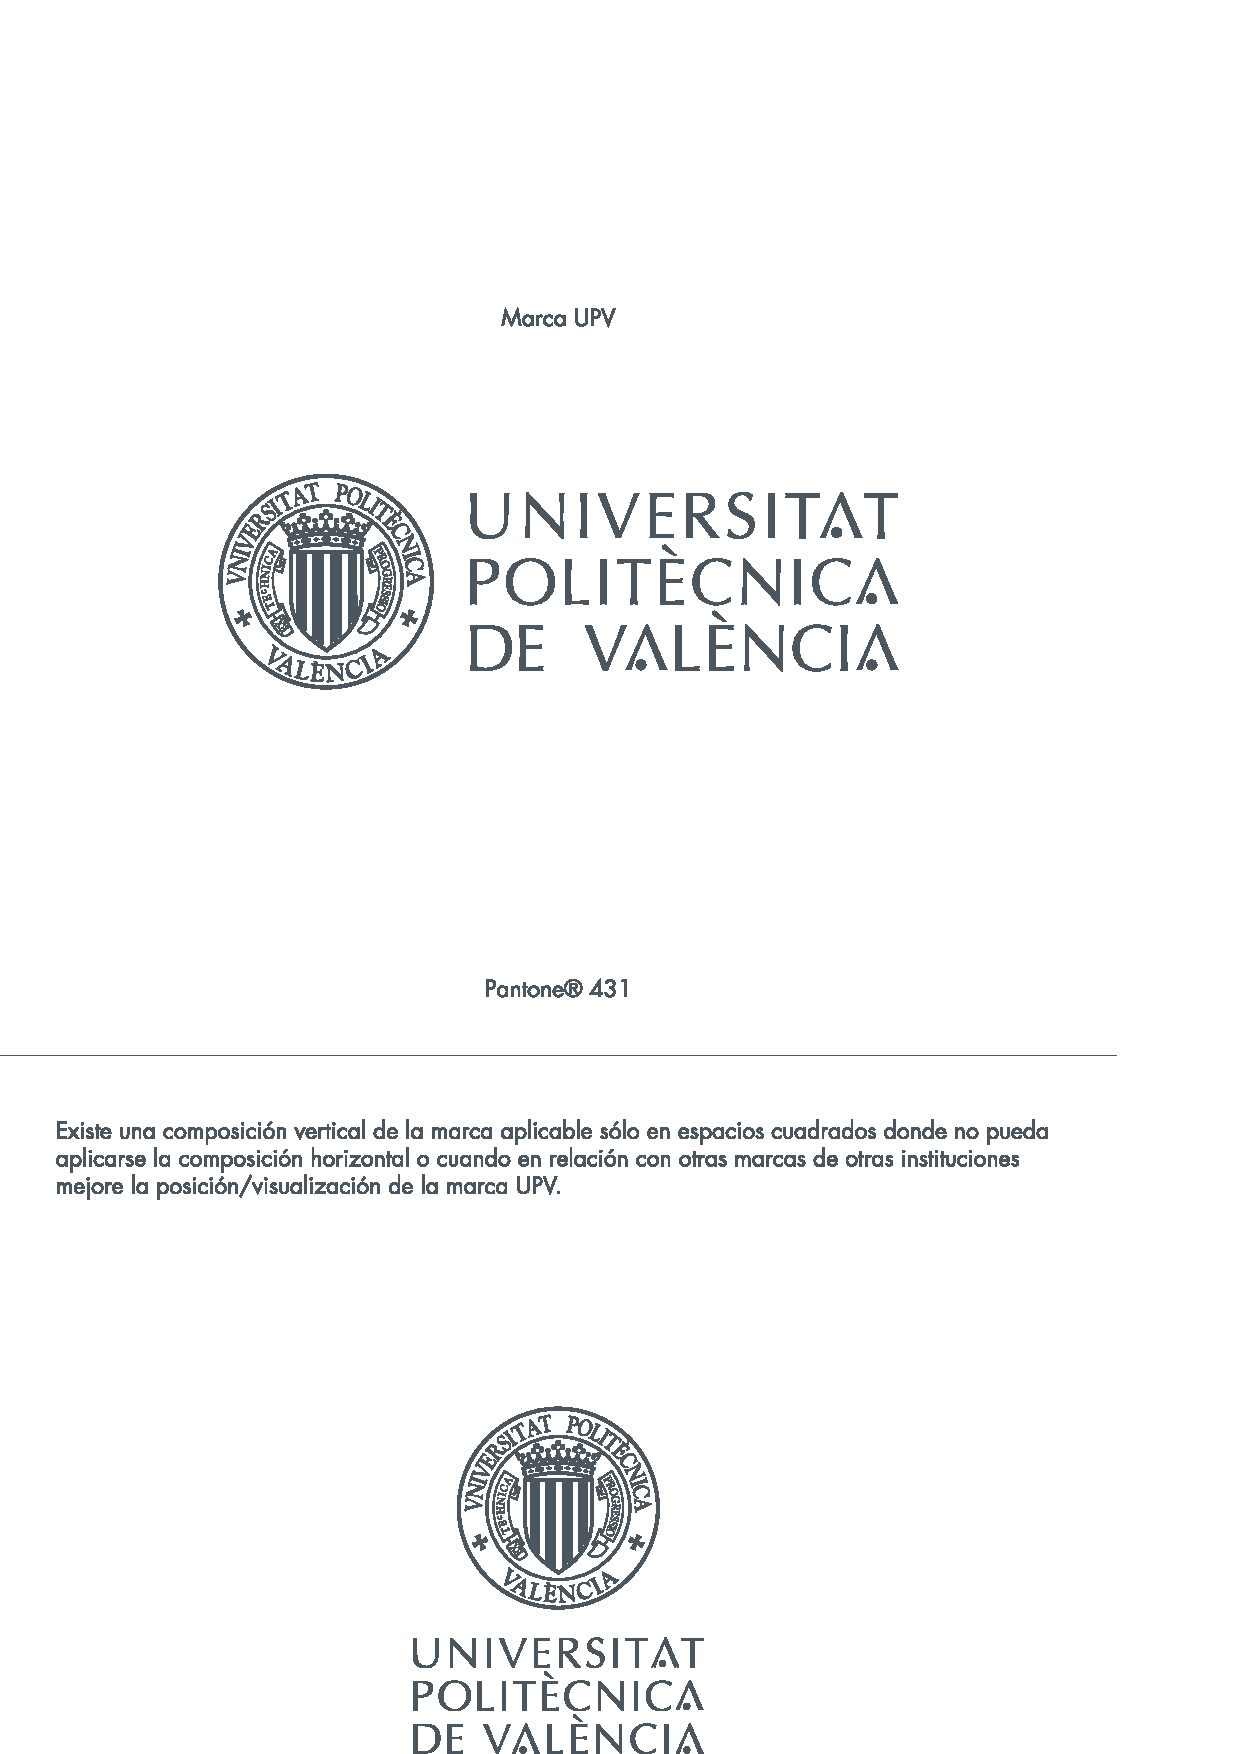
\includegraphics[width=0.4\textwidth]{style/UPV.png}

        \normalsize
        Escuela Técnica Superior de Ingenieros de Telecomunicación\\
        Universidad Politécnica de Valencia\\
        Valencia, España \\
        Septiembre 2019
    \end{center}
\end{titlepage}

\vspace*{\fill}

\noindent \textit{
Dedicado a Fran, porque aún tenemos que hablar de muchas cosas, compañero del alma.
} \vspace*{\fill} \pagenumbering{gobble}

\hypertarget{abstract}{%
\chapter*{Abstract}\label{abstract}}
\addcontentsline{toc}{chapter}{Abstract}

Diabetic Rethinopaty and Age-Related Macular Degeneration are two of the
main causes of blindness all around the globe. However, both diseases
can be treated, and their effects minimized, if they are detected on
early stages. The current screening system is not scalable for the
unstopable growth of both diseases. During this work, three different
automatic screening systems are proposed. These systems use some
convolutional neural networks previously trained on different domains.
The proposed models are more robust and more interpretable than some of
the state-of-the-art ones through the use of more than 39000 images for
training and the use of activation maps during predictions.

\newpage

\hypertarget{resumen}{%
\chapter*{Resumen}\label{resumen}}
\addcontentsline{toc}{chapter}{Resumen}

La Retinopatía Diabética y la Degeneración Macular Asociada a la Edad
son dos de las principales causas de ceguera en todo el mundo. Sin
embargo estas enfermedades pueden ser tratadas, y sus efectos
minimizados, si son detectadas a tiempo. El sistema actual, basado en la
revisión manual de expertos no es viable ante el crecimiento imparable
de ambas. En este trabajo se proponen 3 sistemas para su detección
automática. Estos sistemas usan como punto de partida para su
entrenamiento redes neuronales convolucionales entrenadas previamente en
otros dominios. Las principales ventajas de los sistemas propuestos
frente a los modelos del estado del arte analizados es la robustez que
proporciona haber sido entrenados con más de 39000 imágenes y la gran
interpretabilidad conseguida gracias al uso de mapas de activación en
las predicciones.

\pagenumbering{roman}
\setcounter{page}{1}

\newpage \pagenumbering{gobble}

\tableofcontents

\newpage

\hypertarget{lista-de-figuras}{%
\chapter*{Lista de figuras}\label{lista-de-figuras}}
\addcontentsline{toc}{chapter}{Lista de figuras}

\renewcommand{\listfigurename}{}
\listoffigures

\pagenumbering{roman}
\setcounter{page}{2}

\newpage

\hypertarget{lista-de-tablas}{%
\chapter*{Lista de tablas}\label{lista-de-tablas}}
\addcontentsline{toc}{chapter}{Lista de tablas}

\renewcommand{\listtablename}{}
\listoftables

\pagenumbering{roman}
\setcounter{page}{3}

\newpage

\hypertarget{abreviaciones}{%
\chapter*{Abreviaciones}\label{abreviaciones}}
\addcontentsline{toc}{chapter}{Abreviaciones}

\begin{tabbing}
\hspace{1.0in} \= \hspace{1.5in}  \kill

\textbf{RD}   \> \textbf{R}etinopatía \textbf{D}iabética \\

\textbf{DMAE} \> \textbf{D}egeneración \textbf{M}acular
                 \textbf{A}sociada a la \textbf{E}dad \\

\textbf{NPDR} \> \textbf{N}on-\textbf{P}roliferative
                 \textbf{D}iabetic \textbf{R}etinopathy \\

\textbf{PDR}  \> \textbf{P}roliferative  \textbf{D}iabetic
                 \textbf{R}etinopathy \\

\textbf{ARIA} \> \textbf{A}utomated \textbf{R}etinal
                 \textbf{I}mage \textbf{A}nalyzer \\

\textbf{IA}   \> \textbf{I}nteligencia \textbf{A}rtificial \\

\textbf{CNN}  \> \textbf{C}onvolutional \textbf{N}eural
                 \textbf{N}etwork \\

\textbf{SVM}  \> \textbf{S}upport \textbf{V}ector \textbf{M}achine \\

\end{tabbing}

\newpage
\setcounter{page}{1}
\renewcommand{\thepage}{\arabic{page}}

\hypertarget{intro}{%
\chapter{Introducción}\label{intro}}

Durante este capítulo inicial se presenta el contexto y la motivación
principal detrás de este trabajo, los objetivos perseguidos y la
estructura en la que se plasma toda esta información a lo largo del
mismo.

El presente documento pretende mostrar todas las tareas de investigación
realizadas para la realización del \textbf{Trabajo Final de Máster} que
permite la obtención del título de \textbf{Máster Universitario en
Ingeniería de Telecomunicaciones} de la Universidad Politécnica de
Valencia. Este trabajo supone 30 créditos ECTS (de los 120 créditos
totales de la titulación), lo que equivale aproximadamente a 750 horas
de trabajo.

\hypertarget{motivaciuxf3n}{%
\section{Motivación}\label{motivaciuxf3n}}

La Organización Mundial de la Salud (OMS) estima que, en 2010, 285
millones de personas padecían algún tipo de discapacidad visual. De
ellas, 39 millones eran ciegas. (WHO \& others 2013). El informe
detallaba 7 principales causas de discapacidad visual entre las que se
encontraban las 2 enfermedades que se analizarán en este trabajo: la
\textbf{Retinopatía Diabética} y la \textbf{Degeneración Macular
Asociada a la Edad}. Según se estimaba, el 80\% de estas discapacidades
podrían haberse evitado con las intervenciones adecuadas para su
prevención. En respuesta, la OMS lanzaba su plan de acción que
comenzaría en 2014 y finalizaría en 2019. El informe\footnote{https://www.who.int/blindness/actionplan/en/}
asociado a este plan de acción ponía de manifiesto la necesidad de que
los servicios de salud ocular se convirtieran en parte integral del
sistema primario de salud y se resaltaba la importancia de las campañas
de prevención.

La \textbf{Retinopatía Diabética (RD)} pertenece al grupo de las
enfermedades vasculares, y se ha convertido en la \textbf{principal
causa evitable de ceguera en todo el mundo}. Esta patología se da
actualmente en el 35\% de las personas con diabetes, enfermedad que
afecta al 8.5\% de la población mundial (IAPB 2016), (IDF 2017) . Se
estima que 191 millones de personas sufrirán retinopatía diabética en
2030 (Yingfeng Zheng et~al. 2012). La incidencia de la RD es del 50\% a
partir de los 10 años de la aparición de la diabetes, y del 90\% a
partir de los 30 años (Mookiah, U Rajendra Acharya, Chua, et~al. 2013).

En la Figura \ref{diabetes_dr} se puede observar la previsión esperada
de crecimiento entre 2015 y 2040, tanto en el número de casos de
diabetes, como en el de casos de diabetes que dan lugar a RD.\footnote{Datos
  de https://atlas.iapb.org/vision-trends/diabetic-retinopathy} El
aumento de la población mundial, y el envejecimiento de la misma serán
factores determinantes en este crecimiento, pero también lo serán el
aumento de casos de sobrepeso y la vida sedentaria.

\begin{figure}
\centering
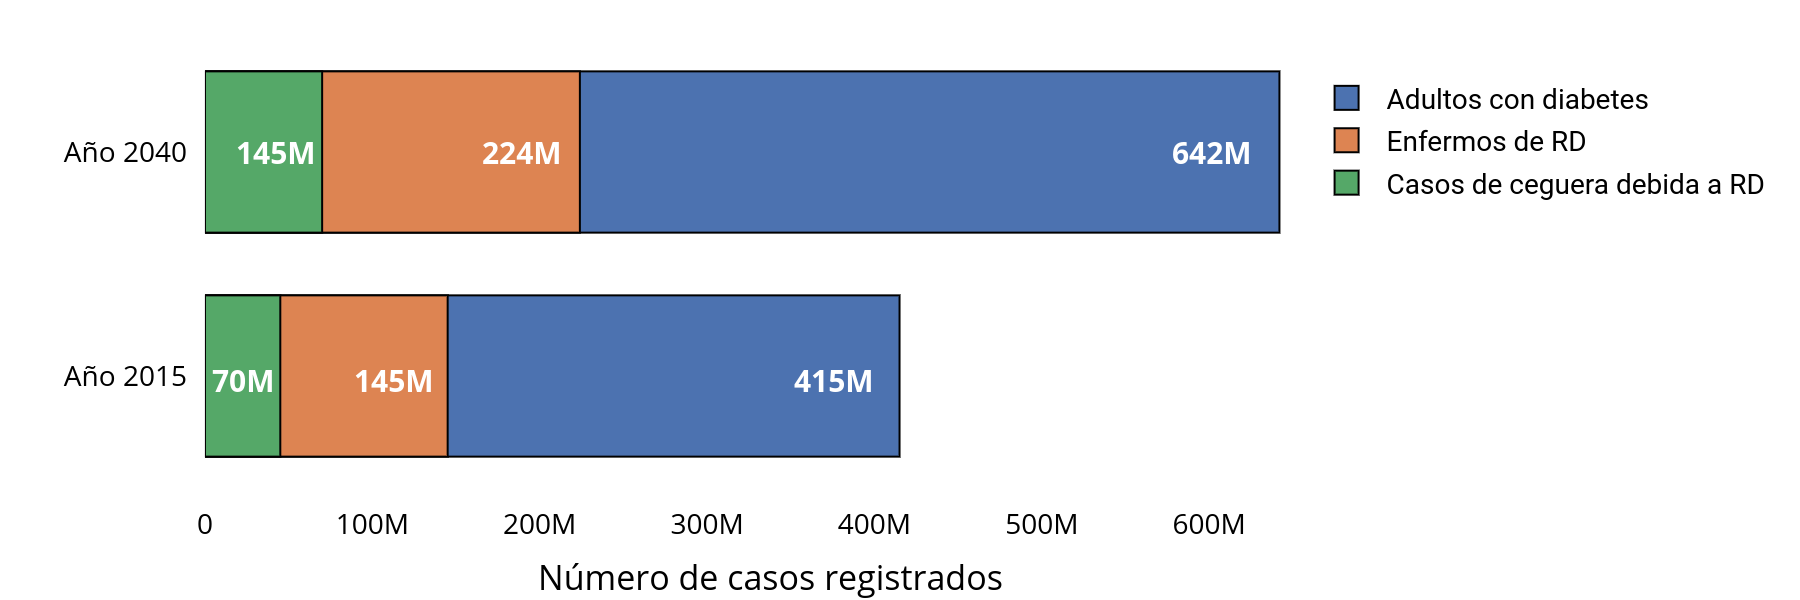
\includegraphics[width=1\textwidth,height=\textheight]{source/figures/stat.png}
\caption{Prevalecencia y previsión de crecimiento de la diabetes y la RD
a nivel mundial. Gráfico de elaboración propia \label{diabetes_dr}}
\end{figure}

La diabetes supone, aproximadamente, el 11.6\% del presupuesto total de
salud de la mayoría de países (Zhang et~al. 2009). Además, el coste de
los pacientes con RD supera notablemente al de los pacientes sin dicha
patología, incrementándose éste con la gravedad de la RD (Zhang et~al.
2017).

Es importante destacar el hecho de que casi el 75\% de las personas que
sufren Retinopatía Diabética pertencen a países en vías de desarrollo
(Mansour 2017), donde no existen los medios adecuados para su detección
temprana ni su tratamiento.

Por otro lado, la \textbf{Degeneración Macular Asociada a la Edad
(DMAE)} es la más común de las enfermedades que afectan a la retina.
Esta patología, de tipo degenerativo, es la \textbf{mayor causa de
ceguera en países desarrollados}, dándose en un 9\% de la población
mundial (Wong et~al. 2014). Hasta el 80\% de los casos de ceguera
causados por esta enfermedad son evitables si son detectados y tratados
a tiempo. (Pascolini \& Mariotti 2012)

El rápido crecimiento de estas enfermedades hace insostenible el sistema
actual basado únicamente en la revisión de expertos. Es necesario
introducir en las clínicas sistemas de detección automática a partir de
imágenes digitales que permitirían agilizar el trabajo de los médicos o
incluso permitir el diagnóstico en zonas donde ni siquiera existen ese
tipo de expertos. Aunque existen diferentes métodos para el diagnóstico
como la tomografía de coherencia óptica (TCO) o la angiografía, el
método más utilizado actualmente se basa en el análisis de
\textbf{imágenes de fondo de ojo} obtenidas mediante cámaras
especializadas (Figura \ref{eidon}). Este tipo de análisis se ha
impuesto al resto de métodos por la facilidad de uso de las cámaras y su
menor coste.

\begin{figure}
\centering
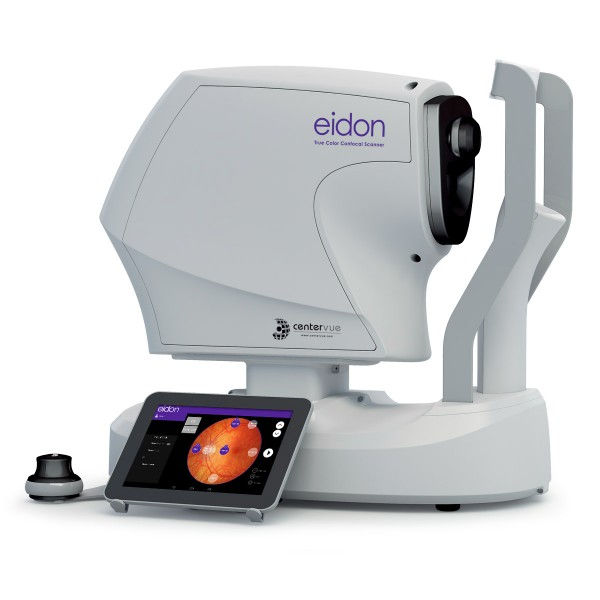
\includegraphics[width=0.4\textwidth,height=\textheight]{source/figures/eidon.jpg}
\caption{Modelo de cámara de fondo de ojo Eidon de la compañía Centervue
\label{eidon}}
\end{figure}

A la fecha de publicación de este trabajo (Septiembre de 2019) aún se
desconoce cuál ha sido el grado de eficacia del plan de acción propuesto
por la OMS, cuyo objetivo principal era la reducción de un 25\% de los
casos de discapacidad visual evitables. Lo que sí que se ha podido
comprobar es el crecimiento experimentado en el número de
investigaciones realizadas en torno a la detección automática de algunas
de estas enfermedades, entrando a la obra nuevos actores como Google que
han permitido dar pasos de gigante en la lucha contra este tipo de
patologías.\footnote{https://ai.googleblog.com/2018/12/improving-effectiveness-of-diabetic.html}

\hypertarget{objetivos}{%
\section{Objetivos}\label{objetivos}}

El objetivo principal de esta investigación ha sido el
\textbf{desarrollo de un sistema de detección automática de Retinopatía
Diabética y Degeneración Macular Asociada a la Edad}. Sin embargo, al
ser este un objetivo amplio, se han establecido una serie de objetivos
más específicos que se detallan a continuación:

\begin{itemize}
\tightlist
\item
  Estudio de la anatomía y fisiología del ojo humano, enfocándose en las
  causas y los efectos de las enfermedades analizadas.
\item
  Análisis y comparación de las principales aproximaciones a la
  detección automática de ambas patologías realizadas hasta la fecha,
  tanto las basadas en Machine Learning como en Deep Learning.
\item
  Diseño, desarrollo y evaluación de diversas topologías de redes
  neuronales convolucionales en la detección de ambas patologías
\item
  Interpretación de las redes convolucionales, tratando de comprender
  qué factores le han ayudado a predecir, en cada caso, la existencia o
  ausencia de la enfermedad.
\end{itemize}

\hypertarget{principales-contribuciones}{%
\section{Principales contribuciones}\label{principales-contribuciones}}

Las principales contribuciones de este trabajo giran en torno a dos
características: la \textbf{robustez} y la \textbf{interpretabilidad}.

\begin{itemize}
\item
  En busca de la \textbf{robustez} se han utilizado más de 39000
  imágenes procedentes de 13 datasets distintos para el entrenamiento de
  los modelos. La combinación de las predicciones de varios
  clasificadores en las predicciones finales de cada sistema también ha
  contribuido a compensar el \emph{overfitting} o \emph{underfitting}
  que pueda tener algún modelo en concreto.
\item
  Para conseguir \textbf{interpretabilidad} se ha diseñado un
  \textbf{Sistema de Predicción e Interpretación} que ha proporcionado
  los valores de confianza de las predicciones, las predicciones de cada
  clasificador por separado, las predicciones combinadas, y los mapas de
  activación.
\end{itemize}

\hypertarget{estructura}{%
\section{Estructura}\label{estructura}}

El presente documento está dividido en los siguientes 7 capítulos:

\begin{enumerate}
\def\labelenumi{\arabic{enumi}.}
\tightlist
\item
  \textbf{\protect\hyperlink{intro}{Introducción}}: Este primer capítulo
  se presenta el problema y la forma en la que éste será abordado en los
  sucesivos capítulos.
\item
  \textbf{\protect\hyperlink{ojo}{El ojo y sus patologías}}: Durante
  este segundo capítulo se estudia la anatomía y fisiología del ojo y se
  analizan las características principales las dos patologías que han
  motivado esta investigación: RD y DMAE.
\item
  \textbf{\protect\hyperlink{ml}{Machine Learning y aplicaciones
  médicas}}: Además de ofrecer una visión general del funcionamiento y
  características de los sistemas de Machine Learning, durante estas
  páginas se muestran ejemplos de las aplicaciones médicas de los
  mismos.
\item
  \textbf{\protect\hyperlink{arte}{Estado del arte en detección de RD y
  DMAE}}: Se analizan las principales aproximaciones para la detección
  de RD y DMAE, tanto de Machine Learning como de Deep Learning,
  publicadas hasta el momento.
\item
  \textbf{\protect\hyperlink{sistema}{Diseño de Sistema de Detección de
  RD y DMAE}}: En este capítulo se muestra el sistema propuesto para la
  detección de RD y DMAE. También se detallan las características de
  todos los conjuntos de imágenes utilizados para el entrenamiento del
  sistema y el sistema adicional para la interpretacción de las
  predicciones.
\item
  \textbf{\protect\hyperlink{resultados}{Análisis de los resultados
  obtenidos}}: Este capítulo detalla las evaluaciones realizadas al
  sistema presentado en el capítulo anterior.
\item
  \textbf{\protect\hyperlink{conclusiones}{Conclusiones}}: Para
  finalizar, se analizan las aportaciones realizadas por esta
  investigación, su aplicabilidad en el mundo real y las posibles líneas
  de investigación futuras que se abren en este momento.
\end{enumerate}

\hypertarget{ojo}{%
\chapter{El ojo y sus patologías}\label{ojo}}

Aunque comúnmente se suele hablar de los ojos como nuestra ventana al
exterior (Zhu et~al. 2001), la realidad es que su funcionamiento y
estructura es considerablemente más complicado que el de una simple
ventana de cristal. Dada su extrema perfección, incluso Charles Darwin
reconoció tener grandes dificultades para explicar los ojos únicamente
mediante variación y selección. (Darwin 2004)

\hypertarget{anatomuxeda-y-fisiologuxeda-ocular}{%
\section{Anatomía y fisiología
ocular}\label{anatomuxeda-y-fisiologuxeda-ocular}}

Los ojos son el principal órgano de la visión. La perfección del ojo es
tal, que cada ojo ha evolucionado adaptándose a las necesidades del
organismo poseedor, lo que ha provocado que existan diversas diferencias
en la anatomía y fisiología ocular de los diferentes organismos. (Zhu
et~al. 2001).

La estructura más simple de ojo consiste en una concentración de células
fotorreceptoras mediante las cuales un organismo puede distinguir, no
sólo la luz y la oscuridad, sino también la dirección de la luz
incidente. Esta última característica supondría, para los organismos con
este tipo de sistema ocular, una ventaja evolutiva ante otros tipos de
organismos que únicamente podrían diferenciar entre luz y oscuridad.

Sin embargo, el sistema óptico complejo presente en el 96\% de las
especies animales, es capaz de realizar un proceso completo que comienza
con la detección de la luz y finaliza con unos impulsos electroquímicos
viajando a través de las neuronas. Durante ese proceso, los ojos tienen
que captar la luz, regular la intensidad mediante un diafragma y,
mediante un sistema de lentes (cristalino), enfocarla en único punto que
se encargará de realizar la transformación en impulsos eléctricos. Este
punto donde convergen todos los rayos de luz, que será objeto de estudio
durante este trabajo, es conocido como \textbf{retina}.

La anatomía y fisiología ocular (Figura \ref{ojohumano}) es similar en
la mayoría de los vertebrados. El globo ocular, que contiene el resto de
elementos del sistema, es una esfera llena de \textbf{humor acuoso}, que
es un líquido compuesto en un 99\% por agua. El constante flujo de este
líquido en el ojo permite regular la presión ocular, de forma que las
propiedades del ojo puedan mantenerse constantes. Además, también
permite aportar nutrientes y oxígeno a la parte anterior del ojo y
eliminar deshechos de esta zona a la que los capilares no son capaces de
llegar (Zhu et~al. 2001).

\begin{figure}
\centering
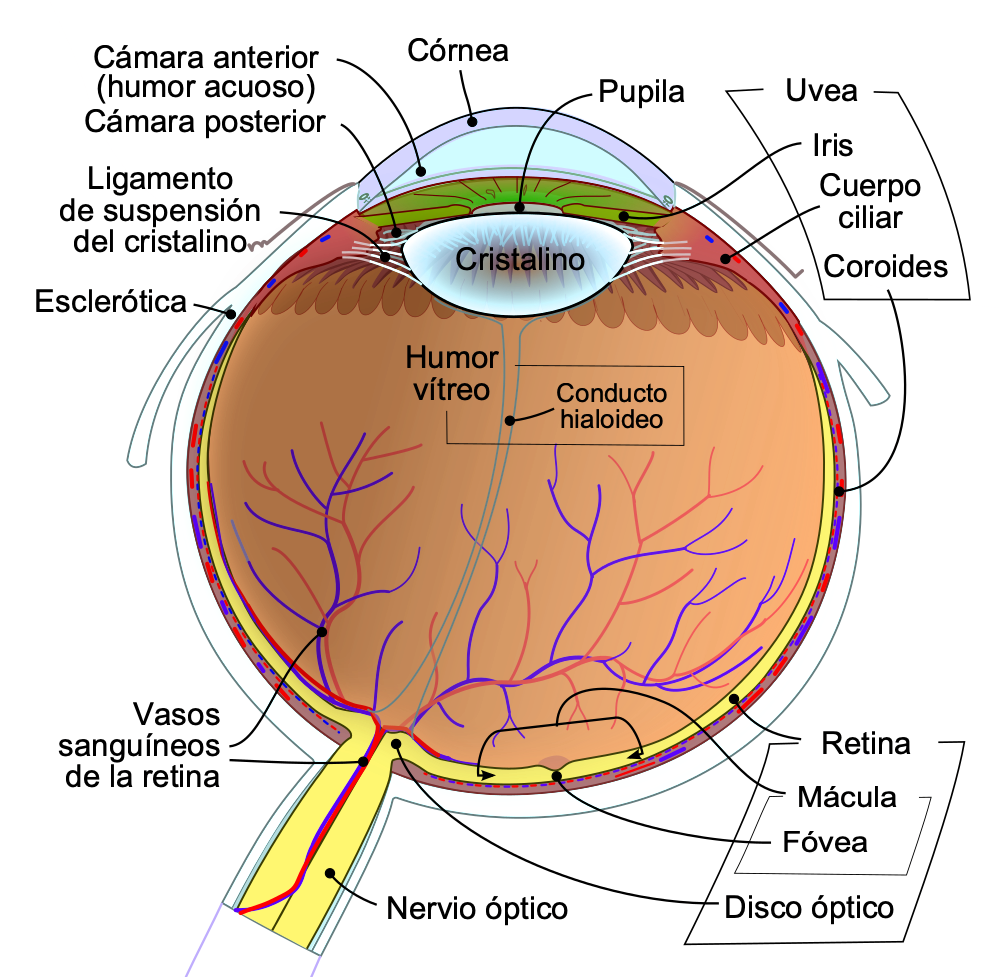
\includegraphics[width=0.8\textwidth,height=\textheight]{source/figures/human-eye.png}
\caption{Estructura del ojo humano. Fuente: Wikipedia \label{ojohumano}}
\end{figure}

La pared del globo ocular la forman 3 capas conocidas como (desde la más
interna a la más externa): \textbf{retina}, \textbf{coroides} y
\textbf{esclerótica}. Cuando la luz llega al ojo, el primer elemento con
el que tiene contacto es la \textbf{córnea}, que pertenece a la capa
esclerótica. Debido a su índice de refracción (mayor que el del aire),
la córnea provocará que se desvíen los rayos de luz que lleguen a ella
permitiendo, así, que converjan en el centro del ojo. La cornea protege
al resto del ojo de polvo, gérmenes y cualquier tipo de sustancia
dañina. Además, también filtra los rayos ultravioleta procedentes de la
luz solar (Zhu et~al. 2001). La mínima dispersión que se produce en los
rayos de luz, que nos permite obtener una imagen clara y definida, está
asegurada por la uniformidad espacial de sus células (Oyster 1999).

Posteriormente, es el \textbf{iris} quien se encargará de contraer o
expandir la \textbf{pupila}, lo que permitirá regular la cantidad de luz
que entra al ojo. Esta es la razón por la que, en condiciones de baja
luminosidad, nuestras pupilas se ven dilatadas, para poder permitir el
paso de la mayor cantidad posible de luz.

A continuación, y como en otros sistemas ópticos artificiales,
necesitamos un elemento que enfoque toda esa luz en un único punto. Este
proceso se realiza mediante el \textbf{cristalino} que actúa como lente,
y una serie de músculos a su alrededor que modifican su forma (y su
índice de refracción) para permitirnos enfocar objetos a diferentes
distancias. Al igual que pasaba con la córnea, es necesario que los
elementos que forman el cristalino tengan un índice de refracción mayor
que el de la córnea y del humor acuoso, lo que le permitirá enfocar
correctamente.

Una vez atravesado el cristalino, la luz llegará a la \textbf{retina}
donde se producirá la transformación de la luz en impulsos eléctricos,
que posteriormente viajarán por el nervio óptico hasta el cerebro, que
será capaz de procesar y comprender la imagen recibida.

\hypertarget{la-retina-y-su-importancia}{%
\subsection{La retina y su
importancia}\label{la-retina-y-su-importancia}}

La palabra \textbf{retina} procede del latín medieval \textbf{rete} o
\textbf{retis} (red). Toma ese nombre debido a la gran red de vasos
sanguíneos que la forman. Utilizando términos de ingeniería, la retina
es el transductor en el proceso de visión. Es la capa de tejido sensible
a la luz situada en el fondo del ojo sin la cual todo el proceso
detallado anteriormente carecería por completo de sentido, puesto que el
cerebro no recibiría la información captada por los ojos. Su color,
rojo, es debido a la inmensa cantidad de vasos sanguíneos que existen
detrás de ella.

A nivel macroscópico, la retina está formada por los siguientes
elementos (Figura \ref{retina}):

\begin{itemize}
\tightlist
\item
  \textbf{Papila o disco óptico}: Conocido como \emph{punto ciego}
  debido a la ausencia de fotoreceptores, es el punto de entrada del
  nervio óptico en el globo ocular. Tiene un diámetro aproximado de 1.5
  mm y forma circular de color amarillo. A través del disco óptico entra
  al globo ocular la arteria central de la retina y sale la vena central
  de la retina. En el disco óptico encontramos también una excavación
  fisiológica conocida como \textbf{cúpula} o \textbf{copa}. Su tamaño,
  y más concretamente, el cociente entre su diámetro y el del disco
  óptico es un buen indicador para la detección de la enfermedad
  conocida como glaucoma.
\item
  \textbf{Arterias y venas}: Son las encargadas de proveer de oxígeno y
  nutrientes a la retina. La arteria central de la retina entra en el
  ojo a través del nervio óptico y se separa en dos ramas, que a su vez
  se separarán formando una extensa red de capilares. Muchas de las
  enfermedades de la vista afectan a estos vasos sanguíneos,
  bloqueándolas o haciéndolas más frágiles.
\item
  \textbf{Mácula}: Esta pequeña área con gran pigmentación se encuentra
  en el centro de nuestra retina. La mácula tiene un diámetro aproximado
  de 5 mm. Es la encargada tanto la visión central como de la visión en
  detalle y en movimiento.
\item
  \textbf{Fóvea}: Es una hendidura en el centro de la mácula, con un
  diámetro aproximado de 1.0 mm que permite enfocar los rayos que llegan
  a la retina.
\item
  \textbf{Retina periférica}: Como su nombre indica, nos permite la
  visión periférica, es decir, la de los rayos de luz que no están en
  nuestro foco central de visión.
\end{itemize}

\begin{figure}
\centering
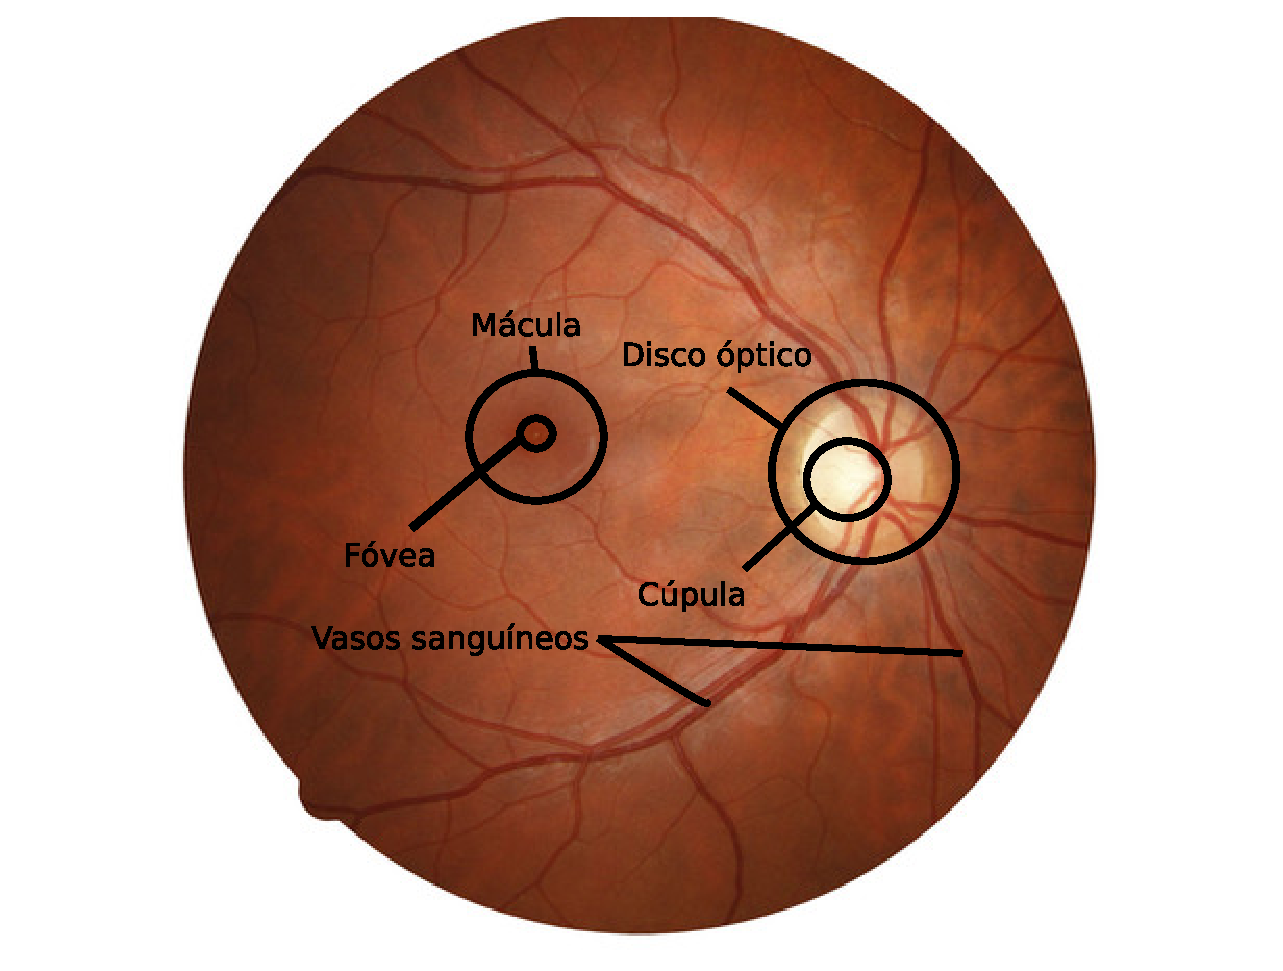
\includegraphics[width=0.9\textwidth,height=\textheight]{source/figures/sitnice.eps}
\caption{Elementos de la retina. Fuente: Kaggle (anotaciones de
elaboración propia) \label{retina}}
\end{figure}

A nivel microscópico, la retina tiene una estructura compleja formada
por varias capas de neuronas interconectadas. Existen dos tipos
principales de fotoreceptores en la retina: los \textbf{conos} y los
\textbf{bastones}. Las células de la retina presentan grandes
similitudes con las del cerebro, apoyando la afirmación común de que el
sistema visual es una extensión del sistema nervioso central (Zhu et~al.
2001).

Estos receptores contienen unos productos químicos conocidos como
\textbf{fotopigmentos}. Los fotopigmentos tienen la propiedad de
descomponerse ante la exposición a la luz, excitando en el proceso a las
fibras nerviosas que salen del ojo.

Los \textbf{bastones} son estructuras cilíndricas y alargadas
extremedamente sensibles a los cambios de intensidad de de la luz. Sin
embargo, no son capaces de percibir información sobre el color. De esto
se encargan los \textbf{conos}, que son células más pequeñas y finas
capaces de de percibir el color y de capturar detalles más finos.

En los \textbf{conos} encontramos tres tipos distintos de fotopigmentos
que responden a diferentes longitudes de onda distinta de la luz. Esto
da lugar a los conocidos como colores primarios de la luz: rojo, azul, y
verde.

En la \textbf{fóvea central}, los únicos fotoreceptores existentes son
los conos, encargados de la visión en detalle y visión en color. Según
nos alejamos de la fóvea y nos dirigimos hacia la parte más periférica
de la retina, los bastones empiezan a ser predominantes. Estos son
responsables de la visión periférica y la visión en bajas condiciones de
luminosidad.

En la retina humana existen aproximadamente 125 millones de
fotoreceptores, de los cuales, aproximadamente 120 millones son bastones
y 5 millones son conos.

Conectadas a los conos y bastones encontramos las \textbf{células
ganglionares}, un tipo de neuronas en la superficie interna de la retina
en las que se produce una diferencia de potencial que se transmite a
través de su largo axón hasta el tálamo, hipotálamo y mesencéfalo del
cerebro. Ya en el cerebro, esta información es procesada e interpretada
por el \textbf{córtex visual}.

\hypertarget{principales-patologuxedas-de-la-retina}{%
\section{Principales patologías de la
retina}\label{principales-patologuxedas-de-la-retina}}

Existen dos tipos principales de enfermedades que afectan a la retina:
las enfermedades vasculares y las degenerativas. Durante este trabajo
analizaremos dos de las más importantes: la \textbf{Retinopatía
Diabética (RD)} y la \textbf{Degeneración Macular Asociada a la Edad
(DMAE)}. En la Figura \ref{enfermedades} podemos ver el efecto que
tienen estas en la visión.

\begin{figure}
\centering
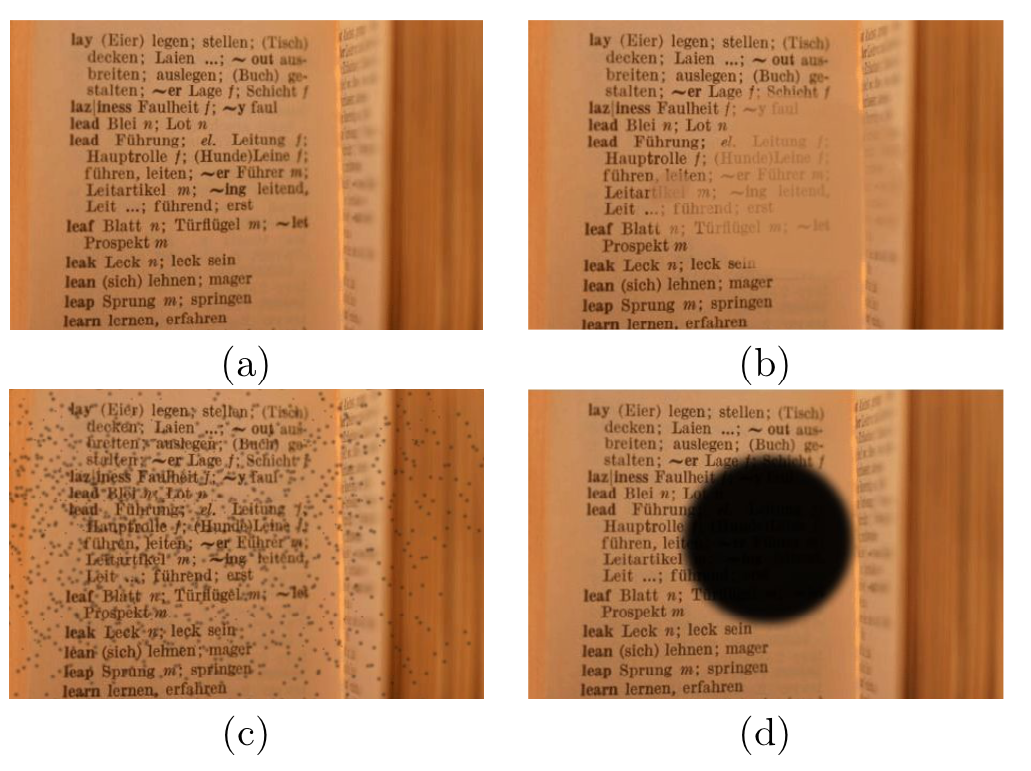
\includegraphics[width=1\textwidth,height=\textheight]{source/figures/vision.png}
\caption{Efectos en la visión de las enfermedades analizadas en este
trabajo: (a) Visión normal, (b) con Retinopatía Diabética no
proliferativa, (c) con Retinopatía Diabética proliferativa y (d) con
degeneración macular asociada a la edad. Fuente: American Academy of
Ophtalmology (www.aao.org) \label{enfermedades}}
\end{figure}

Aún siendo de naturaleza distinta y provocando distintos efectos, ambas
patologías tienen algo en común: \textbf{la mayoría de casos de ceguera
provocados por ellas hubieran podido ser evitados con una detección y
tratamiento de las mismas en los primeros estadios}. La detección de
estas, como veremos más adelante, pasa comúnmente por el análisis de la
retina mediante imágenes de fondo de ojo. Este tipo de imágenes permiten
proyectar la estructura 3D de la retina en un plano 2D. Para captarlas
utilizamos cámaras de fondo de ojo, un tipo especial de cámaras que
cuentan con un microscopio de baja potencia con una cámara adherida,
permitiendo una factor de magnificación de 2.5x. Los rayos de luz viajan
desde la retina a la cámara atravesando la pupila. El sensor de la
cámara es un sensor RGB similar al de otros tipos de cámaras.

\hypertarget{retinopatuxeda-diabuxe9tica}{%
\subsection{Retinopatía Diabética}\label{retinopatuxeda-diabuxe9tica}}

Las personas que sufren de diabetes presentan altos niveles de azúcar en
sangre debido a la incapacidad de su páncreas de generar suficiente
insulina para distribuir el azúcar (Diabetes Tipo I) o a la incapacidad
del organismo de asimilar correctamente la insulina (Diabetes Tipo II).
Estos altos niveles de azúcar pueden producir daños en varios organismos
presentes en nuestro cuerpo.

La Retinopatía Diabética ocurre cuando, debido a la diabetes, se dañan
los vasos sanguíneos de la retina. Es común establecer dos etapas
principales de RD: proliferativa y no proliferativa.

\begin{itemize}
\tightlist
\item
  \textbf{RD No Proliferativa (NPDR)}: Es el primer estadio de la
  enfermedad. Durante esta etapa aparecen microaneurismas, pequeñas
  áreas de inflamación en los vasos sanguíneos de la retina. Además,
  algunos vasos sanguíneos se obstruyen. En casos más complicados, el
  bloqueo de una gran cantidad de vasos sanguíneos provoca que haya
  áreas de la retina que dejen de recibir sangre por completo.
\item
  \textbf{RD Proliferativa (PDR)}: En esta etapa, de mayor gravedad, las
  áreas de la retina que no estaban recibiendo sangre, envían señales al
  cuerpo para que se hagan crecer nuevos vasos sanguíneos. Sin embargo,
  estos nuevos vasos sanguíneos son frágiles y anormales, y en el caso
  de rotura y goteo de sangre, podrían provocar una pérdida severa en la
  visión o incluso resultar en ceguera total.
\end{itemize}

La detección temprana de la RD ha demostrado ser de vital importancia
para evitar la pérdida de vista e incluso la ceguera causada por la
misma. Los primeros estadios de la Retinopatía Diabética son casi
asintomáticos, y no empiezan a afectar a la visión del paciente hasta
que la enfermedad ha avanzado a un estadio en el que el tratamiento es
mucho más complicado y costoso. Se recomienda a los pacientes diabéticos
al menos un análisis anual, para poder aplicar un tratamiento de la
Retinopatía Diabética a tiempo (Fong et~al. 2004).

El tratamiento de la Retinopatía Diabética más común es la
\textbf{fotocoagulación con láser}. Este tratamiento se puede realizar
en una o varias sesiones, tras haber comprobado, mediante una
angiografía fluoresceínica el estado de los vasos sanguíneos. Además,
este tratamiento puede ir acompañado de inyecciones intravítreas de
medicación antangiogénica, que se encargará de evitar el desarrollo
excesivo y anormal de los vasos sanguíneos. En casos de gravedad, puede
ser preciso recurrir a la \textbf{vitrectomía}, una técnica de
microcirugía intraocular.

Las lesiones típicas derivadas de la Retinopatía Diabética son:

\begin{itemize}
\tightlist
\item
  \textbf{Exudados duros}: Son depósitos lipídicos de color amarillento
  brillante y bien definidos, que se filtran procedentes de los vasos
  sanguíneos de la retina. Suelen encontrarse en la capa más externa de
  la misma (Group \& others 1991).
\item
  \textbf{Exudados blandos (o manchas algodonosas)}: Son engrosamientos
  isquémicos de la capa de fibras nerviosas. Presentan bordes difusos y
  un color blanco.
\item
  \textbf{Microaneurismas}: Aparecen normalmente como pequeños grupos de
  puntos rojos con bordes muy definidos. Son causados por la dilatación
  de pequeñas venas, y son uno de los primeros signos de Retinopatía
  Diabética no proliferativa (Williams et~al. 2004). Los microaneurismas
  selen tener bordes bien definidos y su tamaño suele variar entre los
  20\(\mu\)m y 200\(\mu\)m, lo que supone menos de un 8\% del tamaño
  total del disco óptico (Group \& others 1991).
\item
  \textbf{Hemorragias}: Son pequeñas manchas rojas con diversas formas y
  márgenes ligeramente definidos que aparecen en las imágenes de fondo
  de ojo debido a los puntos de sangrado en la retina. Suelen tener un
  tamaño de unos 125\(\mu\)m (Group \& others 1991).
\end{itemize}

En la Figura \ref{lesiones} se observan algunas de las lesiones
descritas anteriormente.

\begin{figure}
\centering
\includegraphics[width=0.7\textwidth,height=\textheight]{source/figures/dr-example.png}
\caption{Lesiones típicas de la Retinopatía Diabética. Elaboración proia
\label{lesiones}}
\end{figure}

Además, como hemos visto anteriormente, en la RD Proliferativa se
produce la neovascularización, aparición de nuevos vasos sanguíneos en
la retina (Figura \ref{vascular}).

\begin{figure}
\centering
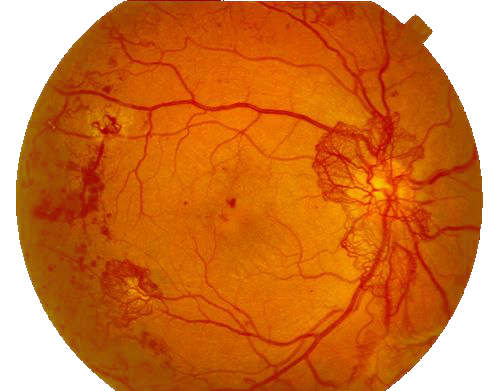
\includegraphics[width=0.7\textwidth,height=\textheight]{source/figures/vascular.png}
\caption{Ejemplo de retina en la que se ha producido neovascularización
\label{vascular}}
\end{figure}

La tabla \ref{estadios_lesiones} nos muestra una posible clasificación
de los diferentes estadios de la Retinopatía Diabética en función de las
lesiones presentes en el paciente.\footnote{Basada en la clasificación
  de https://idrid.grand-challenge.org/grading/} Los pacientes con
Retinopatía Diabética No Proliferativa en grado 3, tienen un 50\% de
probabilidad de desarrollar Retinopatía Diabética Proliferativa en menos
de un año (Mansour 2017).

\begin{longtable}[]{@{}ll@{}}
\caption{Niveles de gravedad de la Retinopatía Diabética en función de
las lesiones observadas \label{estadios_lesiones}}\tabularnewline
\toprule
\begin{minipage}[b]{0.37\columnwidth}\raggedright
Nivel de gravedad\strut
\end{minipage} & \begin{minipage}[b]{0.57\columnwidth}\raggedright
Observaciones\strut
\end{minipage}\tabularnewline
\midrule
\endfirsthead
\toprule
\begin{minipage}[b]{0.37\columnwidth}\raggedright
Nivel de gravedad\strut
\end{minipage} & \begin{minipage}[b]{0.57\columnwidth}\raggedright
Observaciones\strut
\end{minipage}\tabularnewline
\midrule
\endhead
\begin{minipage}[t]{0.37\columnwidth}\raggedright
\textbf{Grado 0}: No RD\strut
\end{minipage} & \begin{minipage}[t]{0.57\columnwidth}\raggedright
Sin ninguna anomalía\strut
\end{minipage}\tabularnewline
\begin{minipage}[t]{0.37\columnwidth}\raggedright
\textbf{Grado 1}: NPDR Ligera\strut
\end{minipage} & \begin{minipage}[t]{0.57\columnwidth}\raggedright
Presencia de algunos microaneurismas\strut
\end{minipage}\tabularnewline
\begin{minipage}[t]{0.37\columnwidth}\raggedright
\textbf{Grado 2}: NPDR Moderada\strut
\end{minipage} & \begin{minipage}[t]{0.57\columnwidth}\raggedright
Presencia de más microaneurismas pero menos que en el grado 3\strut
\end{minipage}\tabularnewline
\begin{minipage}[t]{0.37\columnwidth}\raggedright
\textbf{Grado 3}: NPDR Severa\strut
\end{minipage} & \begin{minipage}[t]{0.57\columnwidth}\raggedright
Alguno de los siguientes:\strut
\end{minipage}\tabularnewline
\begin{minipage}[t]{0.37\columnwidth}\raggedright
\strut
\end{minipage} & \begin{minipage}[t]{0.57\columnwidth}\raggedright
- Más de 20 hemorragias intrarretinales\strut
\end{minipage}\tabularnewline
\begin{minipage}[t]{0.37\columnwidth}\raggedright
\strut
\end{minipage} & \begin{minipage}[t]{0.57\columnwidth}\raggedright
- Dilataciones venosas\strut
\end{minipage}\tabularnewline
\begin{minipage}[t]{0.37\columnwidth}\raggedright
\strut
\end{minipage} & \begin{minipage}[t]{0.57\columnwidth}\raggedright
- Anomalías microvasculares en la retina\strut
\end{minipage}\tabularnewline
\begin{minipage}[t]{0.37\columnwidth}\raggedright
\strut
\end{minipage} & \begin{minipage}[t]{0.57\columnwidth}\raggedright
- Ningún signo de PDR\strut
\end{minipage}\tabularnewline
\begin{minipage}[t]{0.37\columnwidth}\raggedright
\textbf{Grado 4}: PDR\strut
\end{minipage} & \begin{minipage}[t]{0.57\columnwidth}\raggedright
Alguno de los siguientes:\strut
\end{minipage}\tabularnewline
\begin{minipage}[t]{0.37\columnwidth}\raggedright
\strut
\end{minipage} & \begin{minipage}[t]{0.57\columnwidth}\raggedright
- Neovascularización\strut
\end{minipage}\tabularnewline
\begin{minipage}[t]{0.37\columnwidth}\raggedright
\strut
\end{minipage} & \begin{minipage}[t]{0.57\columnwidth}\raggedright
- Hemorragia vítrea\strut
\end{minipage}\tabularnewline
\bottomrule
\end{longtable}

Existen, incluso, estudios que han demostrado que los pacientes que
padecen de Retinopatía Diabética Proliferativa, sufren más riesgo de
tener ataques al corazón, amputaciones o nefropatía diabética (Klein
et~al. 1984), (Cade 2008), (Acharya et~al. 2009).

\hypertarget{degeneraciuxf3n-macular-asociada-a-la-edad}{%
\subsection{Degeneración macular asociada a la
edad}\label{degeneraciuxf3n-macular-asociada-a-la-edad}}

La Degeneración Macular Asociada a la Edad (DMAE) afecta a la mácula
provocando que, quien la sufre, comience a ver imágenes desenfocadas o
deformadas y con zonas oscurecidas. Como se ha explicado previamente, la
mácula permite la visión central, y su degeneración afecta directamente
al día a día del paciente incapacitándolo para hacer tareas comunes como
pueden ser la lectura o la conducción.

Aunque en sus primeros estadios la progresión de la enfermedad sea muy
lenta y el paciente puede que únicamente perciba un ligero cambio en su
visión, en fases avanzadas la DMAE puede provocar la pérdida total de la
visión central. Si es detectada a tiempo, la DMAE puede ser retardada y
mitigada mediante vitaminas y minerales.

El principal signo de DMAE en las imágenes de fondo de ojo es la
aparición de las \textbf{drusas}, depósitos amarillos localizados bajo
la retina, procedentes de la acumulación de minerales. En la Figura
\ref{drusen} se observa la forma de las drusas. En función del número y
tamaño de drusas, podemos definir tres estadios en la enfermedad:

\begin{figure}
\centering
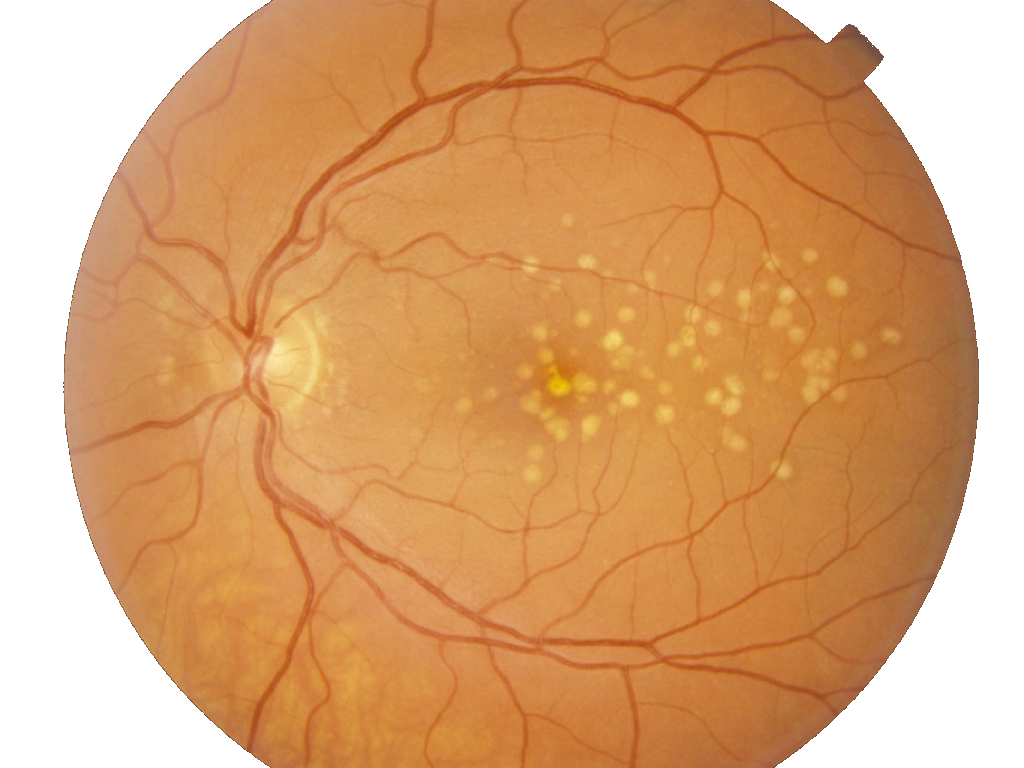
\includegraphics[width=0.8\textwidth,height=\textheight]{source/figures/drusen.png}
\caption{Retina con drusas a causa de DMAE \label{drusen}}
\end{figure}

\begin{itemize}
\tightlist
\item
  \textbf{Estadio inicial}: En este estadio existe un reducido número de
  drusas redondas y de pequeño tamaño (menos de 125 \(\mu\)m). Además,
  estas tienen unos bordes bien definidos. Los pacientes con este grado
  de DMAE no sufren pérdida de visión y tienen un riesgo bajo de
  desarrollar complicaciones (Group \& others 2001).
\item
  \textbf{Estadio intermedio}: En este estadio existen muchas más
  drusas, y estas tienen un tamaño mayor, llegando incluso a aparecer
  algunas de más de 125 \(\mu\)m. Se pueden apreciar cambios en la
  pigmentación de la retina. Cuando las drusas dejan de tener bordes
  definidos, y aparercen en grupos, el riesgo de complicaciones de la
  DMAE es mucho mayor.
\item
  \textbf{Estadio avanzado}: Existen dos subniveles dentro del estadio
  avanzado:

  \begin{itemize}
  \tightlist
  \item
    \textbf{DMAE seca o atrófica}: Se produce por la acumulación de
    desechos que atrofian las células fotosensibles de la zona macular.
    Es la forma más común, y tiene una evolución lenta y progresiva.
  \item
    \textbf{DMAE húmeda o exudativa}: En la DMAE húmeda, crece una
    membrana vascular bajo la retina. De la misma forma que en la
    Retinopatía Diabética Proliferativa, estos nuevos vasos sanguíneos
    son muy frágiles y pueden romperse derramando líquido, lo que
    afectará severamente a la visión.
  \end{itemize}
\end{itemize}

\hypertarget{sistemas-de-diagnuxf3stico}{%
\subsection{Sistemas de diagnóstico}\label{sistemas-de-diagnuxf3stico}}

Uno de los grandes problemas de la Retinopatía Diabética es que no
existe ninguna señal que nos avise en estadios muy tempranos de la
enfermedad, y en el momento que los usuarios deciden hacerse una
examinación, suele ser demasiado tarde para un tratamiento óptimo.

Existen varios tipos de sistemas para el diagnóstico de la RD y DMAE,
entre los que destacan las \textbf{fotografías de fondo de ojo}, la
\textbf{tomografía de coherencia óptica (OCT)} o la
\textbf{angiografía}. La fotografía de fondo de ojo, a diferencia de las
otras dos técnicas, puede ser realizada con sistemas relativamente
baratos y fáciles de manejar y de transportar. Además, las cámaras de
fondo de ojo pueden capturar la información de la retina mediante
técnicas no invasivas. En función de la patología que se intente
diagnosticar, estas imágenes están centradas en la mácula o en el disco
óptico. La Figura \ref{retina} analizada anteriormente para explicar las
partes de la retina, es un ejemplo de las imágenes que proporcionan este
tipo de cámaras, con tamaños de hasta 16 megapíxeles. Es por ello por lo
que la fotografía de fondo de ojo es el sistema más utilizado en los
centros de atención primaria y en el que enfocaremos nuestro estudio.
Sin embargo, cabe destacar que en ocasiones éstas no son suficientes, y
tendrán que ser combinadas con otros tipos de sistemas.

El diagnóstico de la Retinopatía Diabética es tradicionalmente realizado
por oftalmólogos que inspeccionan las imágenes de fondo de ojo en busca
de las diferentes lesiones que caracterizan estas patologías. Sin
embargo, este es un proceso que requiere una gran cantidad de tiempo. La
limitada cantidad de profesionales capaces de realizar este proceso hace
imposible cubrir la demanda actual, que no hace más que crecer (Bjørvig
et~al. 2002). Este hecho es más acusado en zonas rurales o países no
desarrollados donde no es posible el acceso a este tipo de
profesionales. El 75\% de los pacientes de Retinopatía Diabética viven
en áreas donde no existen especialistas ni infraestructura para la
detección y tratamiento de la enfermedad (Guariguata et~al. 2014). Por
ello, diversidad de \textbf{herramientas para el análisis automático de
retina (ARIA)} están siendo desarrolladas actualmente. En este tipo de
herramientas nos centraremos durante el desarrollo de este trabajo.
Éstas llevarán el diagnóstico a sitios donde no sería posible de otra
forma, además de reducir costes y reducir el tiempo necesario para los
diagnósticos en los lugares donde ya se realizaba de forma manual por un
profesional.

Además, según se ha puesto de manifiesto en previos estudios, los
profesionales difieren en numerosas ocasiones en el diagnóstico de los
diferentes estados de este tipo de patologías, debido a que existe un
cierto grado de subjetividad (Ruamviboonsuk et~al. 2005), (Sellahewa
et~al. 2014).

Las técnicas ARIA se basaron en los últimos años en la
\textbf{extracción de manual de caráctrísticas} de las imágenes de fondo
de ojo, que posteriormente se le pasarían a un \textbf{clasificador de
Machine Learning}. Era, por lo tanto, un proceso con dos fases
claramente diferenciadas: \textbf{extracción de características} y
\textbf{clasificación}. Este proceso requería conocimiento experto para
la definición de las características que nos fueran de mayor utilidad
para la detección de la RD y la DMAE.

Con la entrada del \textbf{Deep Learning}, y concretamente las
\textbf{Redes Neuronales Convolucionales (CNN)} este proceso inicial de
extracción de características ha podido ser automatizado, mejorando la
calidad de los sistemas notablemente. Las fases de extracción de
carácterísticas y de predicción se unifican. Las características
extraídas poseen un poder mucho mayor de predicción, puesto que toda la
red ha sido entrenada para ello.

Sin embargo, la naturaleza del problema, la \textbf{falta de
estandarización} y la \textbf{escasa cantidad de imágenes etiquetadas},
han provocado que estos sistemas tuvieran serias dificultades para su
aplicación general.

Esta aproximación al problema del diagnóstico de la RD y DMAE plantea
una serie de preguntas. ¿Cómo se incorporaría un sistema de este tipo en
las consultas? ¿Se introduciría el software en las propias cámaras que
captan la imagen de la retina? ¿Sería posible crear en los países un
sistema centralizado de diagnóstico con imágenes de fondo de ojo?
¿Podrían utilizarse en este sistema centralizado técnicas ARIA
combinadas con las opiniones de expertos? No hay una respuesta para
todas estas preguntas y las ventajas e inconvenientes de algunas de
ellas se desarrollarán en capítulos posteriores.

\hypertarget{ml}{%
\chapter{Machine Learning y aplicaciones médicas}\label{ml}}

Tradicionalmente, el trabajo de los ingenieros de software ha consistido
en dar a las computadoras una serie de reglas explícitas de cómo tienen
que procesar la información para tomar decisiones. Sin embargo, la
complejidad del campo de la medicina es tal que sería prácticamente
imposible capturar toda la información relevante mediante una serie de
reglas definidas de forma explícita (Schwartz et~al. 1986).

El \textbf{Machine Learning} es la rama de la Inteligencia Artificial
que ha permitido crear \textbf{sistemas que aprendan de los datos sin
necesidad de que se programen reglas específicas}. Esto ha supuesto una
auténtica revolución en prácticamente cualquier sector profesional entre
los que, por supuesto, se encuentra también la medicina. Estos sistemas
buscan, de forma automática, \textbf{patrones} en los datos que les
permitan predecir una variable objetivo en función de una serie de
variables de entrada del sistema. De esta forma se crea un
\textbf{modelo} que, idealmente, será capaz de generalizar y obtener la
salida correcta para nuevas entradas nunca vistas. Esto se conoce como
\textbf{Aprendizaje Supervisado} aunque es importante mencionar que no
es la única forma de Machine Learning o Aprendizaje
Automático.\footnote{Existe también, por ejemplo, el Aprendizaje No
  Supervisado, que permite encontrar patrones en los datos aunque no
  exista una variable objetivo a predecir}

Uno de los principales inconvenientes del Machine Learning con respecto
al aprendizaje humano es, a la vez, una de sus principales ventaja: la
\textbf{necesidad de grandes cantidades de datos para su correcto
funcionamiento}. Si se alimentan con una cantidad suficiente de datos,
los algoritmos de Machine Learning podrán encontrar patrones que, para
los humanos, serían prácticamente imposible de detectar. El cerebro
humano es una máquina bastante compleja y sofisticada de encontrar
patrones. Sin embargo, tiene grandes dificultades en realizar el
análisis de datos con alta dimensionalidad. Un modelo de Machine
Learning podrá analizar, en segundos, más pacientes de los que verá un
médico en toda su vida. Además, la cantidad de predictores distintos que
manejará sería totalmente inviable para un humano.

En la Figura \ref{interes-ml} vemos como, a pesar de existir desde los
años 60, el interés de la población en el Machine Learning ha
experimentado un gran ascenso en los últimos años. La democratización
del Machine Learning ha comenzado y multitud de empresas han empezado a
usar modelos predictivos de Aprendizaje Automático en sus procesos.
Existen 3 principales motivos en este crecimiento:

\begin{figure}
\centering
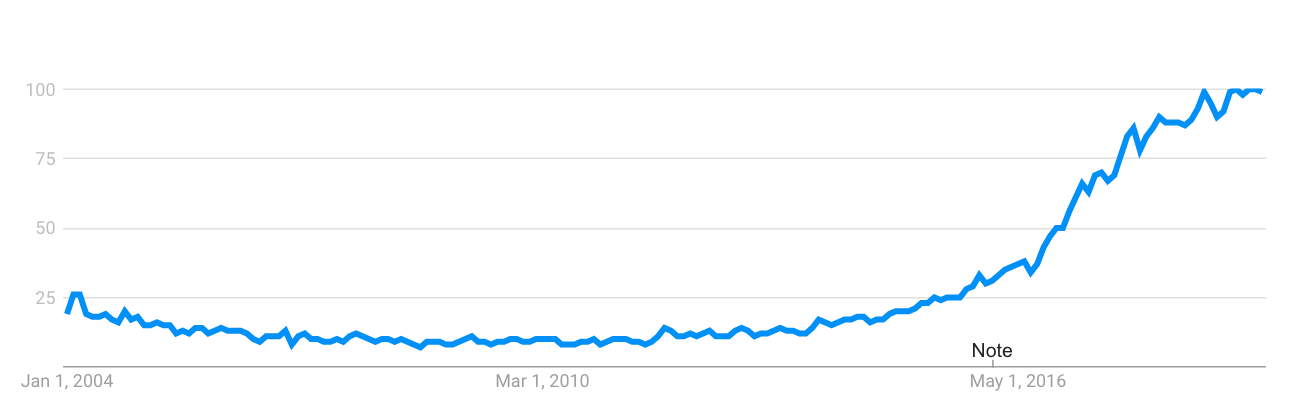
\includegraphics[width=1\textwidth,height=\textheight]{source/figures/interes-ml.png}
\caption{Interés, a lo largo del tiempo y en todo el mundo, del término
Machine Learning en el buscador Google. Datos de Enero de 2014 a Julio
de 2019. Un valor de 100 indica la máxima popularidad del término. Los
valores 50 y 0 indican, respectivamente, que un término es la mitad de
popular en relación con el valor máximo o que no existen suficientes
datos del término. Fuente de los datos: Google Trends
\label{interes-ml}}
\end{figure}

\begin{itemize}
\tightlist
\item
  \textbf{Nuevos algoritmos}: Principalmente en la rama del Deep
  Learning, en los últimos años se ha producido una serie de importantes
  avances. Sin embargo, este no es el factor principal del crecimiento,
  pues la mayoría de algoritmos que se están implantando en muchas
  compañías existen desde hace varias décadas.
\item
  \textbf{Mayor capacidad de computación}: Sin duda, este ha sido un
  factor clave en el crecimiento de estas técnicas. Además, la entrada
  al mercado de las tarjetas gráficas o GPUs ha permitido paralelizar
  los procesos consiguiendo ejecuciones cientos de veces más rápidas.
\item
  \textbf{Mayor cantidad de datos}: Todos estos algoritmos no podrían
  aportar valor de no existir ingentes cantidades de datos, tanto
  estructurados como no estructurados, en los que poder encontrar
  patrones. Con el creciente uso de servicios online y la expansión del
  IoT o Internet de las Cosas se están generando mayor cantidad de datos
  cada día que nunca antes se había generado. Según Forbes, el 90\% de
  los datos existentes en 2018 en todo el mundo, se generaron entre 2016
  y 2017.\footnote{https://www.forbes.com/sites/bernardmarr/2018/05/21/how-much-data-do-we-create-every-day-the-mind-blowing-stats-everyone-should-read/}
\end{itemize}

\hypertarget{ia-big-data-machine-learning-y-deep-learning}{%
\section{IA, Big Data, Machine Learning y Deep
Learning}\label{ia-big-data-machine-learning-y-deep-learning}}

Inteligencia Artificial, Big Data, Machine Learning, Deep Learning;
actualmente existe mucha confusión en el uso de estos términos. Aunque
comparten características, no tienen el mismo significado. En este
apartado se detallarán las similitudes y diferencias entre todos ellos
para evitar el lenguaje inexacto usado habitualmente, principalmente, en
publicidad y medios de comunicación.

Comenzaremos por el \textbf{Big Data}, pues es el término más vago y
confuso. Cuando hablamos de Big Data nos referimos al análisis de
grandes cantidades de datos que no podrían ser analizados con técnicas
convencionales de computación. Sin embargo, las líneas que marcan las
fronteras del Big Data están difusas, y a menudo es un término más
utilizado por medios de comunicación y falsos gurús que por
profesionales técnicos y académicos.

Por otro lado, los campos de la \textbf{Inteligencia Artificial (IA)},
el \textbf{Machine Learning} y el \textbf{Deep Learning} sí que están
más claramente definidos aunque, el hecho de que cada uno de ellos sea
un subcampo del anterior (Figura \ref{ia-ml}), a menudo da lugar a
confusión. Llamamos \textbf{Inteligencia Artificial} a un conjunto de
técnicas que tratan de que los ordenadores imiten, de alguna forma, el
comportamiento humano.

\begin{figure}
\centering
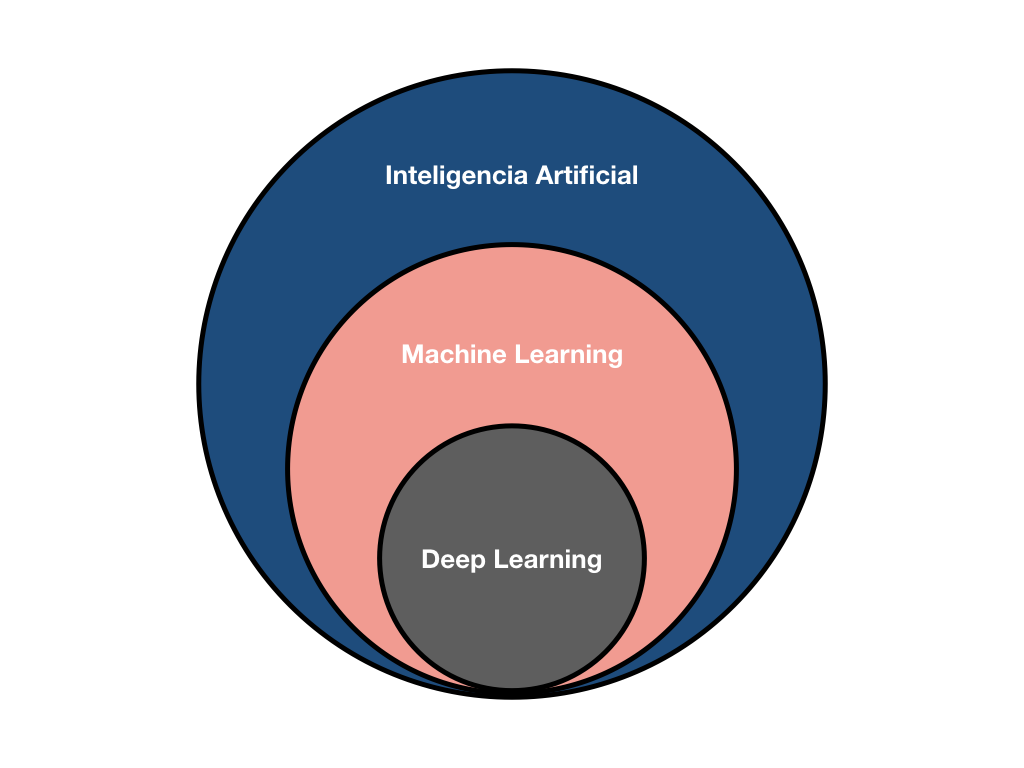
\includegraphics[width=0.8\textwidth,height=\textheight]{source/figures/ia-ml.png}
\caption{El Machine Learning es un campo perteneciente a la Inteligencia
Artificial. El Deep Learning, a su vez, es un campo dentro del Machine
Learning. Elaboración propia \label{ia-ml}}
\end{figure}

El \textbf{Machine Learning} es un subcampo dentro de la IA, que
consiste en un conjunto de técnicas y herramientas, principalmente
estadísticas, que permiten a los ordenadores obtener patrones a partir
de grandes conjuntos de datos. Gracias a esos patrones seremos capaces
de entender mejor los datos o hacer predicciones. La forma más común de
Machine Learning es el conocido como \textbf{Aprendizaje Supervisado}.
Durante el entrenamiento de los modelos de Aprendizaje Supervisado, se
proporcionan al algoritmo una serie de datos históricos. Entre ellos se
encuentra la \textbf{variable objetivo}, es decir, la que posteriormente
querremos predecir en los nuevos datos de entrada. Por ejemplo, en un
modelo de detección de cáncer a partir de imágenes médicas, nuestra
variable objetivo será precisamente la que indique si una imágen
pertenece a un paciente enfermo de cáncer o un paciente sano. Esta
variable, por lo tanto, tendrá dos posibles valores, siendo este un
problema de \textbf{clasificación}. En los problemas de clasificación se
tratan de predecir \textbf{variables discretas o clases}, es decir,
variables que solo pueden tomar un rango limitado de posibles valores.
Si, por ejemplo, realizáramos un modelo para predecir el precio de una
vivienda en función de sus características, nos encontraríamos ante un
problema de \textbf{regresión}, pues el precio es un valor contínuo.

Es común en los algoritmos para aprendizaje supervisado el uso de una
\textbf{función de coste}. Esta función mide el error entre las
predicciones del modelo y los datos reales. De forma iterativa, muchos
de los algoritmos de Aprendizaje Automático tratarán de ajustar una
serie de parámetros (o pesos) intentando minimizar esta función. Un
claro ejemplo de algoritmos con este comportamiento son las conocidas
como \textbf{redes neuronales}, de las que explicaremos su
funcionamiento en el siguiente apartado.

Precisamente las redes neuronales, son las que dan lugar al \textbf{Deep
Learning}. Cuando añadimos más complejidad a las redes neuronales somos
capaces de detectar patrones mucho menos evidentes, además de tratar
problemas complejos sin necesidad de un pre-procesamiento manual previo
de los datos que los simplifique. Este pre-procesamiento sí que es
necesario en muchos proyectos de Machine Learning y, de hecho, supone un
importante porcentaje del tiempo de trabajo de los ingenieros de Machine
Learning. Los algoritmos de Deep Learning son actualmente el estado del
arte en tareas como reconocimeiento de imágenes (Krizhevsky et~al.
2012), reconocimiento del habla (Deng et~al. 2013), procesamiento del
lenguaje natural (Collobert et~al. 2011), análisis de información de
aceleradores de partículas (Baldi et~al. 2014) o reconstrucción de los
circuitos cerebrales (Helmstaedter et~al. 2013), entre muchas otras.

Como vemos en la Figura \ref{interes-ai} el término Big Data, que
durante mucho tiempo estuvo en cabeza en popularidad, ha perdido fuerza
en los últimos años mientras que Machine Learning y Deep Learning (en
menor medida) siguen creciendo.

\begin{figure}
\centering
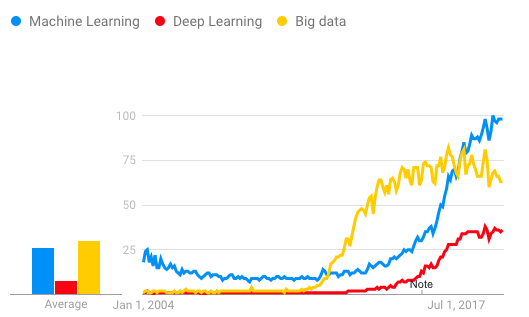
\includegraphics[width=0.8\textwidth,height=\textheight]{source/figures/interes-ai.png}
\caption{Interés, a lo largo del tiempo y en todo el mundo, de los
término Machine Learning (en azul), Deep Learning (en rojo) y Big Data
(en amarillo) en el buscador Google. Datos de Enero de 2014 a Julio de
2019. Un valor de 100 indica la máxima popularidad del término. Los
valores 50 y 0 indican, respectivamente, que un término es la mitad de
popular en relación con el valor máximo o que no existen suficientes
datos del término. Fuente de los datos: Google Trends
\label{interes-ai}}
\end{figure}

\hypertarget{redes-neuronales-descenso-de-gradiente-y-backpropagation}{%
\section{Redes neuronales, descenso de gradiente y
backpropagation}\label{redes-neuronales-descenso-de-gradiente-y-backpropagation}}

Una red neuronal consiste en un conjunto de nodos, conocidos como
\textbf{neuronas}, conectados entre si para transmitirse señales. Estas
neuronas suelen estar dispuestas en una serie de \textbf{capas}, en las
que, comúnmente, cada neurona de una capa está conectada a todas las
neuronas de las capas anteriores. De esta forma, la salida de unas
neuronas pasa a ser la entrada de otras (Figura \ref{neural-network}).

\begin{figure}
\centering
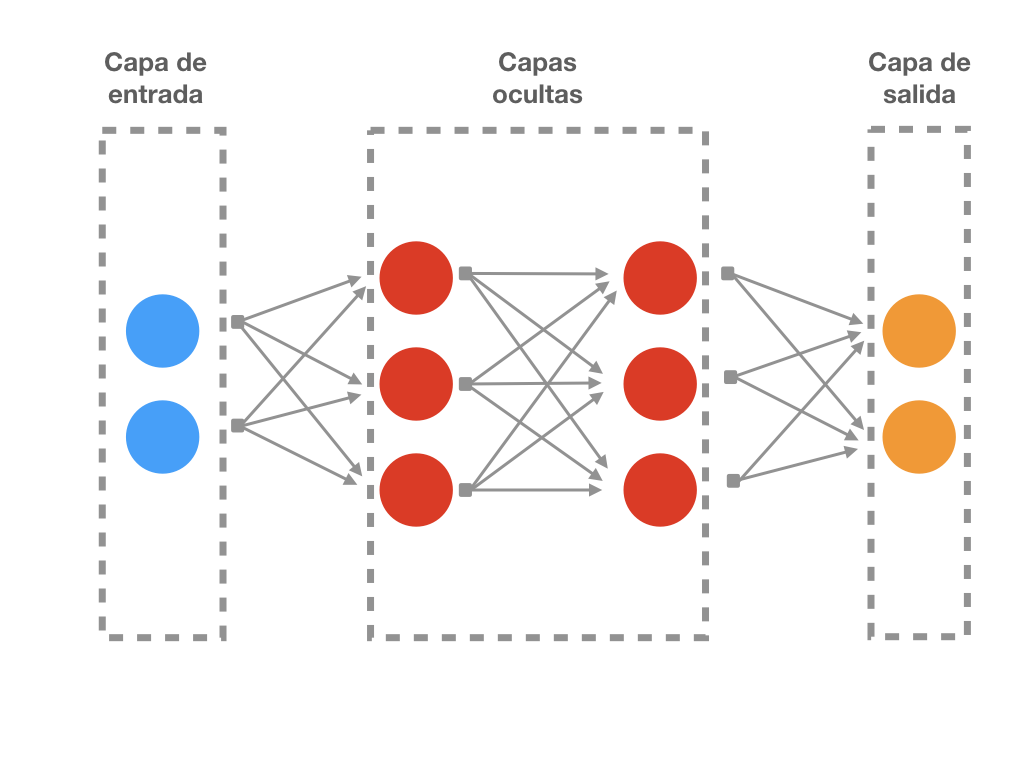
\includegraphics[width=0.9\textwidth,height=\textheight]{source/figures/neural-network.png}
\caption{Representación de una red neuronal con dos capas ocultas. Cada
uno de los círculos representa una neurona. Elaboración propia
\label{neural-network}}
\end{figure}

\begin{figure}
\centering
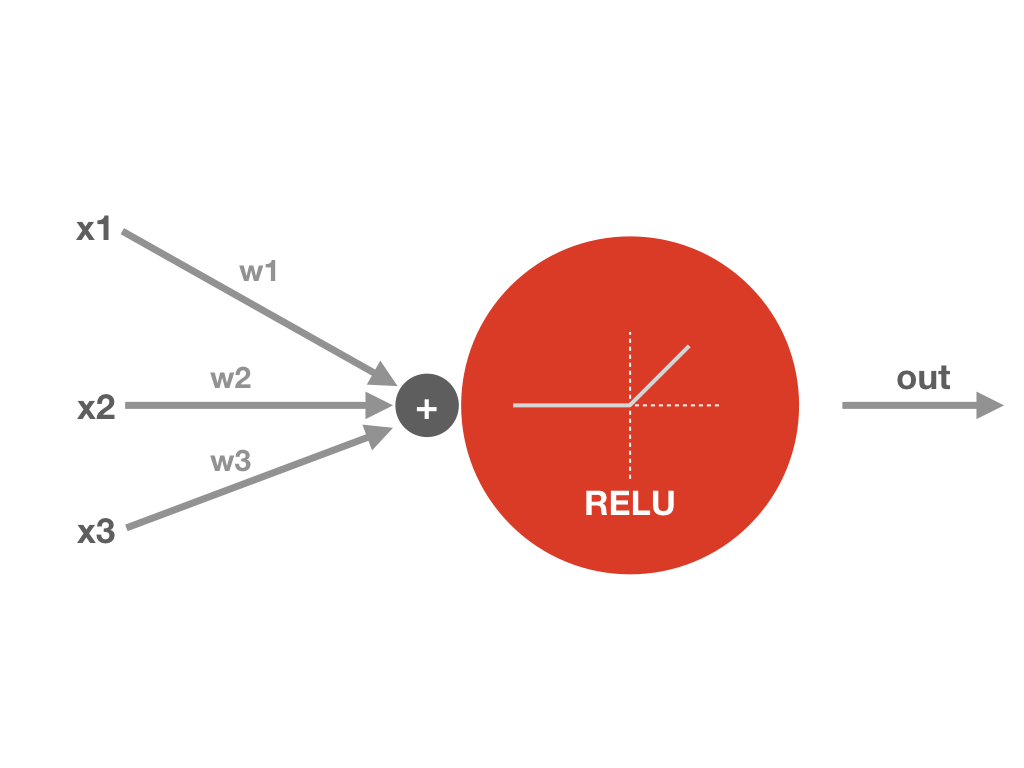
\includegraphics[width=0.9\textwidth,height=\textheight]{source/figures/single-neuron.png}
\caption{Representación de una sola neurona con 3 entradas. Cada una de
esas entradas tiene asociado un peso. La neurona utiliza la función de
activación ReLU. Elaboración propia \label{single-neuron}}
\end{figure}

La Figura \ref{single-neuron} representa las operaciones realizadas por
una sola neurona durante la predicción. Estas mismas operaciones son
realizadas en todas las neuronas de la red. Cada neurona combina sus
entradas con un conjunto de coeficientes o pesos. Las entradas
\(x_1,x_2,x_3\) y los pesos \(w_1,w_2,w_3\) son números reales, que
pueden ser positivos o negativos.\footnote{Aunque no se haya
  representado, también existe un término adicional, \emph{b} (término
  de sesgo), que no está multiplicado por ningún peso y se suma a z} El
nombre de \textbf{peso} se debe a que la función de estos, al
multiplicarse por los valores de las entradas es definir la importancia
de cada una de ellas. En cada una de las neuronas, los resultados de
todos estos productos se suman (ecuacion \ref{eq:train1}) y se pasa el
valor obtenido a lo que se conoce como \textbf{función de activación}
(ecuacion \ref{eq:train2}) , que añade un comportamiento no-lineal al
proceso que permite modelar funciones curvas o no triviales.
Actualmente, la función de activación más utilizada es la \textbf{ReLU}
(Rectified Linear Unit)\footnote{Otras funciones de activación usadas
  comúnmente son \textbf{softmax}, \textbf{tangente hiperbólica} o la
  \textbf{función sigmoide}} cuya fórmula podemos ver en la ecuación
\ref{eq:relu}.

\begin{equation} \label{eq:relu}
f(z)=max(z,0)
\end{equation}

\begin{equation} \label{eq:train1}
 z = x_1w_1 + x_2w_2 + x_3w_3 + b
\end{equation}

\begin{equation} \label{eq:train2}
  out = max(z,0)
\end{equation}

Como vemos en la ecuación \ref{eq:train3}, las ecuaciones anteriores
pueden ser generalizadas para cualquier número de entradas.

\begin{equation} \label{eq:train3}
 out(X) = max(\sum_{i}x_iw_i+b,0)
\end{equation}

Durante el \textbf{entrenamiento}, los pesos cambian de valor,
intentando minimizar la función de coste. Suponiendo que \(y\) es el
valor real de la variable objetivo para un conjunto de entradas \(X\),
la función de coste \(L(X,y)\) podría ser simplemente la de la ecuación
\ref{eq:train4}.

\begin{equation} \label{eq:train4}
 L(X,y) = (out(X) - y)^2
\end{equation}

Para ajustar el vector de pesos se suele calcular el vector de
gradiente. Este vector indica, para cada peso, cómo se modificaría el
error si ese peso se aumentara ligeramente. Es decir, nos proporciona la
pendiente de la función de coste (o función de pérdidas). El vector de
pesos es entonces ajustado en el sentido opuesto al vector de gradiente
(ecuación \ref{eq:train5}), bucando así \textbf{minimizar el error}. El
valor \(\alpha\) representa lo que conocemos como \textbf{learning rate}
o \textbf{factor de aprendizaje} y se encarga de controlar la velocidad
a la que la red neuronal aprende. Es muy importante la elección correcta
de este parámetro, pues, un valor demasiado bajo supondrá que la red
tarde muchas iteraciones en encontrar el mínimo de la función de coste.
Sin embargo, un valor demasiado alto puede suponer que la red no sea
capaz de converger y encontrar este mínimo. Este proceso completo es lo
que conocemos como \textbf{descenso de gradiente}.

\begin{equation} \label{eq:train5}
 w_{ij} =  w_{ij} - \alpha\frac{\partial L(X,y)}{\partial w_{ij}}
\end{equation}

En la práctica, este proceso no usa todos los datos cada vez sino que se
utiliza el \textbf{Descenso de Gradiente Estocástico} (SGD por sus
iniciales en inglés). Gracias al SGD podemos actualizar los pesos de
nuestra red neuronal tomando cada vez un pequeño conjunto de datos
(conocido como \textbf{batch}).

El origen de las redes neuronales es el \textbf{Perceptrón},
desarrollado en los años 60, que era una red simple de una sola capa de
entrada y una capa de salida. Sin embargo, fue en los años 80 cuando
estas comenzaron a desarrollar su verdadero potencial gracias al
algoritmo de \emph{backpropagation}, que permitió que se añadieran
nuevas capas intermedias a las redes neuronales, conocidas como
\textbf{capas ocultas}. La técnica de \emph{backpropagation} no es más
que una aplicación de la regla de la cadena de las derivadas que permite
propagar el error calculado al final de la red a todas las capas de
ésta. En la ecuación \ref{eq:train6} podemos ver un ejemplo de como
aplicar la regla de la cadena de las derivadas para obtener la derivada
de la función de coste en función de los pesos. De la misma forma,
podríamos aplicar la regla de la cadena para obtener la derivada de la
función de coste en función de los pesos de varias capas atrás.

\begin{equation} \label{eq:train6}
 \frac{\partial L(X,y)}{\partial  w_{ij}} =  \frac{\partial L(X,y)}{\partial out(X)} \frac{\partial out(X)}{\partial  w_{ij}}
\end{equation}

Gracias a la técnica de \emph{backpropagation}, podemos propagar el
error a lo largo de las capas, para calcular en cada una el vector de
gradiente y actualizar con él los pesos. El \emph{backpropagation} ha
permitido, por lo tanto, añadir \textbf{nuevas capas intermedias} a las
redes.

Estas capas intermedias permiten encontrar patrones más complejos, y
dieron lugar a lo que conocemos como \textbf{Deep Learning}. Si no
tuviéramos \textbf{capas ocultas}, nuestras redes únicamente
encontrarían relaciones directas entre las entradas y las salidas. Sin
embargo, las capas ocultas nos permiten modelar de forma mucho más
acertada el mundo real, donde las salidas dependen de las interacciones
y combinaciones entre las distintas entradas. Estrictamente hablando,
nos referimos a Deep Learning cuando tenemos una red con más de una capa
oculta. El Deep Learning permite crear modelos computacionales
compuestos de múltiples capas de procesamiento que son capaces de
aprender representaciones de los datos con \textbf{múltiples capas de
abstracción} (LeCun et~al. 2015).

En las redes profundas, cada capa de neuronas se entrena,
automáticamente, en un conjunto de características distinto en base a la
salida de la capa anterior. A medida que avanzamos a través de la red,
las características que las neuronas son capaces de detectar son más
complejas, ya que agregan y recombinan características de capas
anteriores. Esta propiedad, conocida como \textbf{jerarquía de
características}, hace posible que este tipo de redes sean capaces de
tratar datasets de muy alta dimensionalidad. Las redes neuronales
profundas realizan por lo tanto \textbf{extracción automática de
características} sin la necesidad de la intervención de un humano (LeCun
et~al. 2015).

Otra técnica a destacar, que será usada en los sistemas diseñados, es la
técnica del \textbf{dropout}. Esta técnica de regularización trata de
evitar el sobreajuste de la red ignorando de forma aleatoria, durante el
entrenamiento, la salida de algunas neuronas. De esta forma, se fuerza a
la red neuronal a encontrar patrones más robustos, evitando así que
aprenda el \emph{ruido} de nuestro conjunto de datos.

\hypertarget{redes-neuronales-convolucionales}{%
\subsection{Redes neuronales
convolucionales}\label{redes-neuronales-convolucionales}}

La capacidad de las redes neuronales de encontrar patrones complejos en
datasets con una gran cantidad de dimensiones las convierte en
candidatas perfectas para tareas como la clasificación de imágenes o el
reconocimiento de voz. Sin embargo, estos clasificadores necesitan un
trabajo manual previo de extracción de características cuando tratan con
señales (imágenes, audios, etc).

La aparición de las \textbf{Redes Neuronales Convolucionales (CNN por
sus siglas en inglés)} permitió eliminar la extracción de
características y delegarla en el propio algoritmo de
\emph{backpropagation}. De esta forma, es posible usar como entradas de
nuestro modelo los \emph{datos en bruto} (píxeles de las imágenes o
muestras de audio). Un momento clave para las redes convolucionales fue
en 2012, en el \textbf{ImageNet Large Scale Visual Recognition Challenge
(ILSVRC)}\footnote{http://image-net.org/challenges/LSVRC/} cuando una
solución novedosa basada en CNNs (Krizhevsky et~al. 2012) obtuvo, de
forma holgada, la primera posición en la competición.

La arquitectura de las redes convolucionales está basada en la
organización de la corteza visual del cerebro humano. En él, existen
neuronas individuales que responden a estímulos en una región delimitada
del campo visual. Este tipo de redes son muy similares a las redes
neuronales tradicionales analizadas anteriormente. De la misma forma que
éstas, las CNN también están compuestas de neuronas dispuestas en capas
y se busca minimizar una función de coste mediante el ajuste de una
serie de pesos. Sin embargo, las CNN, al asumir que tendrán imágenes
como entradas, pueden realizar tareas más especializadas que evitarán la
carga computacional que supondría tratar cada píxel de la imagen como un
input más de una red neuronal convencional.

Una de las principales ventajas de las redes neuronales convolucionales
con respecto a otras aproximaciones al problema es que las CNN poseen un
cierto grado de \textbf{invarianza a la distorsión y al desplazamiento}.
Esto permite que podamos usar este tipo de redes sin apenas
pre-procesamiento de las imágenes.

Las CNN constan de \textbf{capas convolucionales} y \textbf{capas de
reducción (o pooling)} alternadas.

En las \textbf{capas de convolución} se aplican una serie de
\textbf{filtros} a las imágenes (cuyos pesos son parámetros modificados
durante el entrenamiento por el algoritmo de \emph{backpropagation}). En
ellas se producen también las \textbf{transformaciones no lineales
(ReLU)}. Cada uno de los filtros se desplazará sobre toda la imagen
calculándose, en cada posición, el producto escalar entre la región de
la imagen y los valores del filtro. Este proceso, la
convolución\footnote{Aunque es común en la literatura hablar de este
  proceso como convolución, en realidad este cálculo en tratamiento
  digital de señal es conocido como una correlación cruzada. (Goodfellow
  et~al. 2016)} de la imagen con el filtro, es el que da nombre a estas
capas. Estos filtros hacen de \textbf{detectores de características}.
Precisamente el desplazamiento de ese filtro por toda la imagen es lo
que nos permitirá detectar formas y patrones en cualquier posición de la
imagen, consiguiendo así la deseada invarianza al desplazamiento. En la
Figura \ref{lena} podemos ver el efecto de la convolución sobre una
imagen.

\begin{figure}
\centering
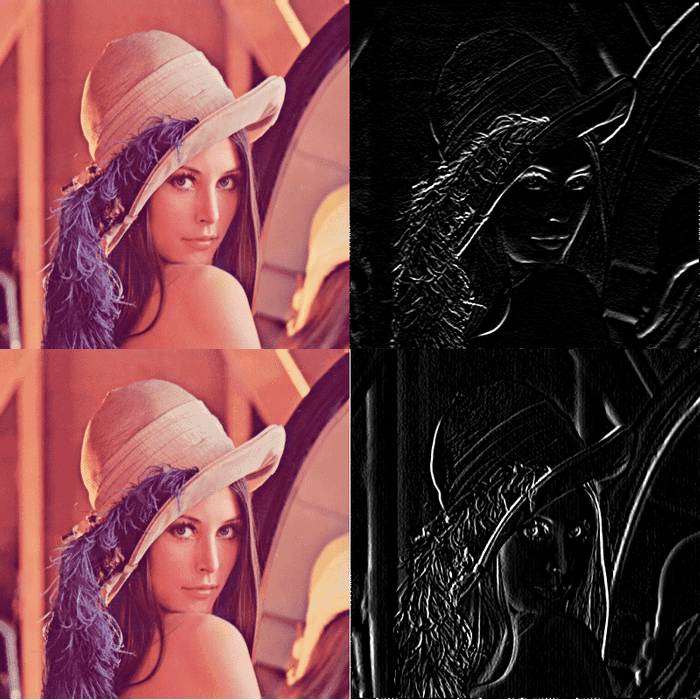
\includegraphics[width=0.8\textwidth,height=\textheight]{source/figures/lena.png}
\caption{Resultado de la convolución de una imagen con un filtro Sobel
de 3x3 horizontal (arriba) y otro vertical (abajo) Fuente:
https://victorzhou.com/blog/intro-to-cnns-part-1/ \label{lena}}
\end{figure}

En las \textbf{capas de reducción o pooling} se disminuye la cantidad de
parámetros. Para ello, se obtiene el promedio o el máximo de una serie
de regiones, reduciendo así el tamaño del mapa de características y
contribuyendo a evitar el \emph{overfitting}. En función de si se
obtiene el promedio o el máximo de las regiones, estas capas son de
\textbf{Max Pooling} o de \textbf{Average Pooling}. La Figura
\ref{maxpool} representa este proceso.

\begin{figure}
\centering
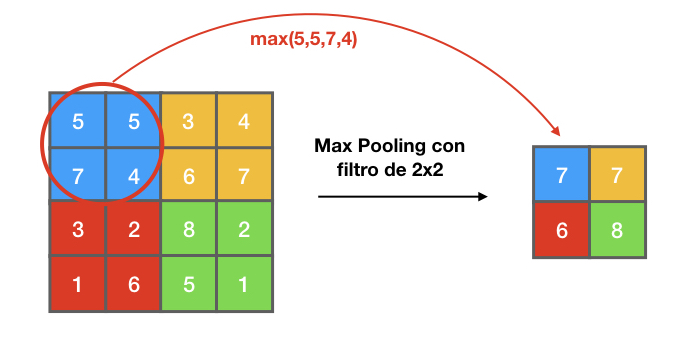
\includegraphics[width=0.8\textwidth,height=\textheight]{source/figures/maxpool.jpeg}
\caption{Representación del proceso de Max Pooling con un filtro de 2x2
sobre una imagen de 4x4. Elaboración propia \label{maxpool}}
\end{figure}

Al final de todas estas capas tenemos las \textbf{Fully Connected
Layers}, capas como las de las redes tradicionales que, a partir de los
parámetros extraídos por las capas convolucionales y de pooling,
realizan las clasificaciones o regresiones finales.

La Figura \ref{conv} representa todo este proceso en un ejemplo de
reconocimiento de dígitos en imágenes. En ella podemos ver la salida de
los filtros de las dos capas convolucionales que tiene la arquitectura
del ejemplo.

\begin{figure}
\centering
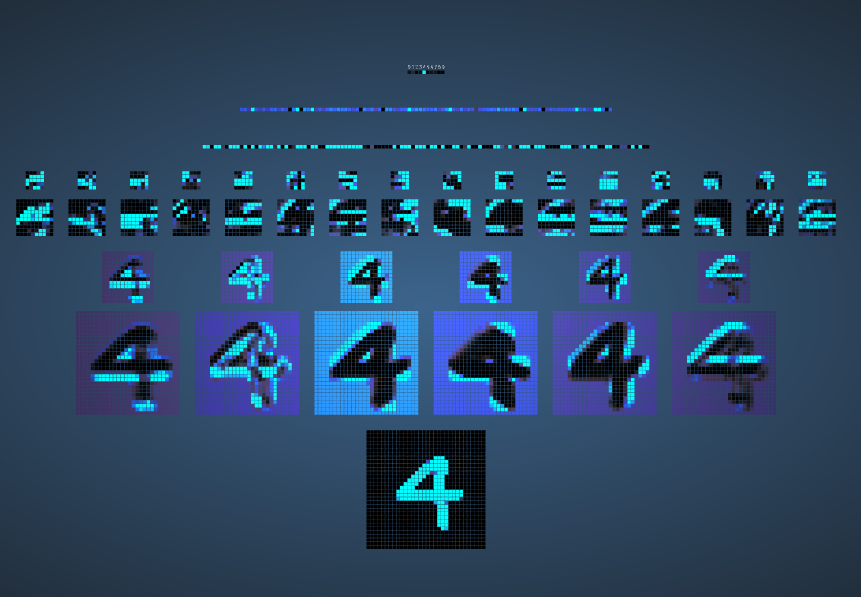
\includegraphics[width=1\textwidth,height=\textheight]{source/figures/conv.png}
\caption{Representación de los mapas de activación de una red
convolucional con 2 capas convolucionales y 3 fully-connected. Cada capa
convolucional va seguida de una de max pooling. Fuente:
http://scs.ryerson.ca/\textasciitilde aharley/vis/conv/flat.html
\label{conv}}
\end{figure}

El funcionamiento del algoritmo de \emph{backpropagation} en las redes
convolucionales es practicamente igual que en las no convolucionales,
por lo que no supone demasiada dificultad teórica añadida para el
entrenamiento. La red será capaz de encontrar, durante el entrenamiento,
los pesos de los filtros que permitan extraer las características
adecuadas para predecir correctamente nuestra clase objetivo.

Las CNN explotan la propiedad de que, los patrones detectados, no son
más que composiciones de otros patrones más simples. En una imágen, por
ejemplo, mediante la composición de varias líneas simples damos lugar a
motivos que, de nuevo mediante composición, dará lugar a las formas de
los objetos. La detección de cada uno de estos niveles de abstracción
corresponderá a unas capas concretas de nuestra red convolucional,
siendo las primeras capas las que detectarán características más simples
como líneas, bordes o colores y las últimas capas las que detectarán
elementos compuestos mucho más complejos. Esto es conocido como la
\textbf{jerarquía de las capas}.

Existe una gran cantidad de arquitecturas de redes convolucionales, que
han demostrado ser eficaces en diversos campos. Ejemplos de ellas pueden
ser las siguientes:

\begin{itemize}
\tightlist
\item
  \textbf{LeNet}: Fue, en 1998, una de las primeras arquitecturas de
  CNNs (LeCun et~al. 1998). Su propósito era, principalente, el
  reconocimiento de dígitos en imágenes. Era una red pequeña con 7
  capas, siendo dos de ellas convolucionales, otras dos de tipo pooling
  y el resto fully-connected.
\item
  \textbf{Alexnet}: Fue la ganadora en 2012 del concurso ILSVRC
  (Krizhevsky et~al. 2012), con una arquitectura similar a LeNet pero
  más profunda, con cerca de 60 millones de parámetros y haciendo uso,
  entre otras novedades, de la función de activación ReLU.
\item
  \textbf{VGGNet}: Fue presentada en 2014 (Simonyan \& Zisserman 2014),
  y aún sigue siendo la arquitectura preferida por la comunidad para la
  extracción de características de imágenes. Fue la primera arquitectura
  de CNNs realmente profunda (19 capas). Se caracteriza por ser una
  arquitectura muy uniforme que usa únicamente filtros de 3x3. Sin
  embargo, era muy costosa de entrenar, puediendo llegar a tener hasta
  140 millones de parámetros.
\item
  \textbf{ResNet}: Presentada un año después a la VGGNet (He et~al.
  2016), se caracteriza por tener saltos entre capas. La salida de la
  \textbf{capa i} puede ser la entrada de la \textbf{capa i+2}.
\item
  \textbf{Inception}: La primera versión de esta arquitectura (Google
  Net) (Szegedy et~al. 2015) introdujo immportantes novedades entre las
  que destacaba el uso de varios filtros de distintos tamaños en el
  mismo nivel, cuyas salidas serían concatenadas. El objetivo era crear
  redes \emph{más anchas} en vez de \emph{más profundas}.
\end{itemize}

\hypertarget{transfer-learning}{%
\section{Transfer Learning}\label{transfer-learning}}

La mayoría de métodos de Machine Learning asumen que los datos de
entrenamiento y los de test vienen de la misma distribución y espacio
funcional (Pan \& Yang 2009). Por ello, cuando esta distribución cambia,
debemos volver a entrenear nuestros modelos desde 0, obteniendo datos
totalmente nuevos. El \textbf{Transfer Learning}, sin embargo, mediante
la transferencia de conocimiento entre modelos, permite transferir
información de un modelo entrenado previamente a un modelo nuevo que
está siendo entrenado en otro conjunto de datos distinto.

El Transfer Learning es una técnica de Machine Learning que permite
utilizar un modelo desarollado para una tarea específica como punto de
partida para otra tarea distinta (aunque relacionada). Además de
permitirnos obtener clasificadores de forma mucho más rápida
aprovechando el conocimiento previo, el Transfer Learning hace posible
el uso del Deep Learning con conjuntos de datos pequeños con los que
sería imposible entrenar una red desde 0. El Transfer Learning es
considerado por muchos investigadores como un paso más en dirección
hacia la AGI.\footnote{Artificial General Intelligence: Aquella
  inteligencia artificial que puede realizar con éxito cualquier tarea
  intelectual de cualquier ser humano}

\hypertarget{transfer-learning-con-imuxe1genes}{%
\subsection{Transfer Learning con
imágenes}\label{transfer-learning-con-imuxe1genes}}

En la práctica, cada vez es menos común el entrenamiento de redes
convolucionales \emph{from scratch}. Existen 2 principales motivos:

\begin{itemize}
\tightlist
\item
  En determinados ámbitos, no siempre existen datasets con una gran
  cantidad de imágenes, suficiente para entrenar una red convolucional
  desde cero.
\item
  Aún existiendo dicho dataset, el tiempo necesario para su completo
  entrenamiento puede ser de días, semanas o incluso meses dependiendo
  del equipo usado, la cantidad de datos y la complejidad de la
  arquitectura de la red.
\end{itemize}

Existen tres principales estrategias a la hora de realizar Transfer
Learning:

\begin{itemize}
\tightlist
\item
  \textbf{Red convolucional como extractor de características}: Como se
  ha analizado anteriormente, una red convolucional puede ser vista como
  una herramienta para extraer características de las imágenes que
  posteriormente serán usadas por capas \emph{fully connected} (o por
  cualquier otro tipo de clasificador) para realizar la clasificación.
  Conociendo esto, podemos utilizar la red convolucional entrenada para
  un conjunto de imágenes en otro conjunto de imágenes distinto, siendo
  el clasificador final el único que tendrá que ser reentrenado.
\item
  \textbf{Fine-tuning de la red convolucional} Como se ha analizado
  anteriormente, las capas iniciales de las redes convolucionales se
  encargan de detectar características más generales y patrones simples,
  que van siendo más complicados a medida que avanzamos hacia capas
  posteriores. Por lo tanto, es común que estas primeras capas tengan
  siempre contenidos similares incluso en modelos entrenados con
  diferentes conjuntos de imágenes. Estas capas podrán ser
  reaprovechadas, con lo que únicamente tendremos que reentrenar las
  últimas capas y el clasificador final.
\item
  \textbf{Modelos pre-entrenados}: Este tercer caso supone el
  reentrenamiento total de la red, sin embargo, partiendo de unos pesos
  que han sido previamente entrenados en otro conjunto de imágenes. De
  esta forma se consigue que el número de iteraciones necesarias hasta
  llegar al nivel de exactitud requerido sea menor.
\end{itemize}

Los criterios para decidir qué estrategia de Transfer Learning usar en
cada caso dependen principalmente de las diferencias de contenido y
tamaño entre las imágenes de nuestro dataset y las del dataset original
(con el que se entrenó el modelo que vamos a reutilizar)

Es común usar las siguientes \emph{rules of thumb} como guía en función
de 4 posibles escenarios:\footnote{http://cs231n.github.io/transfer-learning/}

\begin{itemize}
\tightlist
\item
  \textbf{El nuevo dataset es pequeño pero similar al original}: Al
  tratarse de un dataset pequeño, modificar las capas convolucionales de
  nuestro modelo original puede dar lugar a \textbf{sobreajuste}. Por lo
  tanto, y puesto que las imágenes de ambos datasets son similares, la
  estrategia adecuada será utilizar la red convolucional como extractor
  de características y entrenar únicamente el clasificador final.
\item
  \textbf{El nuevo dataset es grande y similar al original}: En este
  caso, como tenemos más imágenes podremos realizar fine-tunning de la
  red sin miedo a caer en sobreajuste.
\item
  \textbf{El nuevo dataset es pequeño y muy diferente al original}: De
  nuevo, al tener un dataset pequeño, descartaremos entrenar la red
  convolucional. En este caso, lo que haremos es entrenar solo un
  clasificador. Además, al ser las imágenes distintas a las del dataset
  original, no podremos aprovechar las últimas capas de la red
  convolucional que serán eliminadas.
\item
  \textbf{El nuevo dataset es grande y muy diferente al original}: En
  este caso entrenaremos la red convolucional al completo. Sin embargo,
  será de utilidad comenzar nuestro entrenamiento a partir de un modelo
  pre-entrenado.
\end{itemize}

\newpage

\hypertarget{explicabilidad-las-redes-convolucionales}{%
\section{Explicabilidad las redes
convolucionales}\label{explicabilidad-las-redes-convolucionales}}

Para la introducción de técnicas basadas en Deep Learning en diversos
sectores profesionales (siendo la medicina uno de ellos), tan importante
como la exactitud de las predicciones, es la existencia de técnicas que
permitan \textbf{explicar el por qué de esas predicciones} o, al menos,
dar un valor de \textbf{confianza} para cada una. Aunque las redes
neuronales sean generalmente consideradas como \textbf{cajas negras}, en
los últimos años han aparecido nuevas técnicas que permiten entender los
factores que han llevado al clasificador a tomar una u otra decisión.
Concretamente, durante este trabajo, se hará uso de una técnica para la
interpretación de redes neuronales convolucionales conocida como
\textbf{Mapas de Atención}, técnica basada en \textbf{Gradient-weighted
Class Activation Mapping (Grad-CAM)} (Selvaraju et~al. 2017). Gracias a
estos mapas podemos conocer cuáles son las zonas de una imagen que más
han influido en una predicción. Para ello, esta técnica usa los
gradientes específicos de cada clase que fluyen hasta la última capa
convolucional para producir un mapa de calor con las zonas de interés
para la detección de esa clase (Figura \ref{gradcam}).

\begin{figure}
\centering
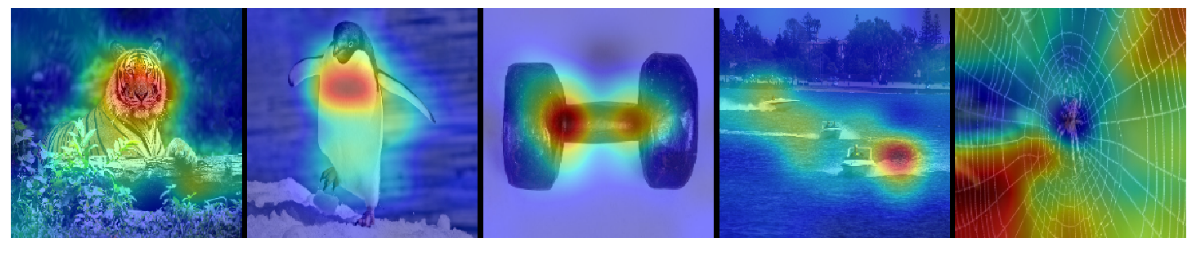
\includegraphics[width=0.7\textwidth,height=\textheight]{source/figures/grad-cam.png}
\caption{Mapas de atención generados por Grad-Cam para distintas clases
de Imagenet. Fuente: https://github.com/raghakot/keras-vis
\label{gradcam}}
\end{figure}

Esta técnica no requiere modificar la arquitectura de la red ni volver a
entrenarla. Además, permite obtener la localización aproximada de los
objetos detectados en la imagen, aunque durante el entrenamiento no se
haya utilizado ningún tipo de información de localización.

\hypertarget{aplicaciones-muxe9dicas-del-machine-learning}{%
\section{Aplicaciones médicas del Machine
Learning}\label{aplicaciones-muxe9dicas-del-machine-learning}}

¿Cómo sería un sistema sanitario en el que cada decisión relacionada con
una enfermedad, en lugar de ser tomada por una sola persona, fuera
tomada por un conjunto de los principales expertos del mundo de esa
enfermedad? Esa es la pregunta que se hacen multitud de investigadores
(Rajkomar et~al. 2019). Estos concluyen que los tratamientos recetados
de esta forma, y no los más conocidos por una única persona que los
prescribe, serían los más efectivos. Además, se evitaría el
\textbf{error humano}. Por desgracia, un sistema de este tipo sería
inviable debido principalmente a la falta de expertos, que no darían
abasto para diagnosticar a millones de pacientes cada día. Sin embargo,
el Machine Learning nos promete un sistema similar a este pero realmente
viable y escalable, con la capacidad de \textbf{aplicar todas las
lecciones recogidas de la experiencia colectiva} en cada una de las
decisiones, sin que esto genere una gran carga de trabajo para unos
pocos expertos.

Hace ya 50 años se ponía de manifiesto la necesidad de \emph{``aumentar,
o incluso remplazar las funciones intelectuales de los médicos''}
(Schwartz 1970). Además, la implementación de los \textbf{Historiales
Clínicos Electrónicos} en diversidad de sistemas de salud, proporciona
una ingente cantidad de datos que podrían ser de gran utilidad para la
creación de modelos de Machine Learning de todo tipo.\footnote{Aunque no
  hay que olvidar las limitaciones derivadas de la privacidad y la
  protección de datos}

El uso de herramientas estadísticas en medicina no es ninguna novedad.
Desde antes de la irrupción de las técnicas más novedosas de Machine
Learning y Deep Learning, la estadística descriptiva tenía un papel
fundamental, estando prácticamente siempre presente en los artículos de
las revistas de medicina. Son necesarias técnicas estadísticas que nos
permitieran estudiar la eficacia de los fármacos o los factores de
riesgo de determinadas enfermedades.

La rama de la \textbf{epidemilogía}, cuyos orígenes se sitúan hacia el
siglo IV a.C., trata de recopilar y tratar los datos de los pacientes y
sus patologías, para estudiar la frecuencia y distribución de los
diversos fenómenos relacionados con la salud. La epidemilogía trata de
encontrar patrones en las enfermedades centrándose principalmente en
tres aspectos: tiempo, lugar y persona. Gracias a ella somos capaces de
definir los problemas de salud más importantes de una comunidad, además
de sus factores de riesgo. Con esta información podremos desarrollar
programas de prevención o control, e incluso predecir tendencias de una
enfermedad.

Sin embargo, la revolución del Machine Learning y el Deep Learning de
los últimos años se empieza a hacer notar, aunque de forma más lenta que
en otros campos, en la medicina. Por primera vez, este tipo de técnicas
salen del ámbito de la investigación y son utilizadas para el
\textbf{diagnóstico}. Tradicionalmente los programas utilizados en
diagnóstico eran \textbf{sistemas expertos}. Este tipo de programas
simplemente se limitaban a pedir una serie de datos sobre el paciente, y
obtenían conclusiones a partir de una serie de reglas que previamente
habían tenido que ser definidas por especialistas. Sin embargo, con
sistemas basados en Machine Learning, \textbf{estas reglas son
automáticamente inferidas a partir de datos históricos} (Figura
\ref{tradicional}). Una de las principales características del Machine
Learning, que le hace destacar sobre otros métodos tradicionales, es su
capacidad de manejar enormes cantidades de predictores y encontrar
complicados patrones en ellos.

\begin{figure}
\centering
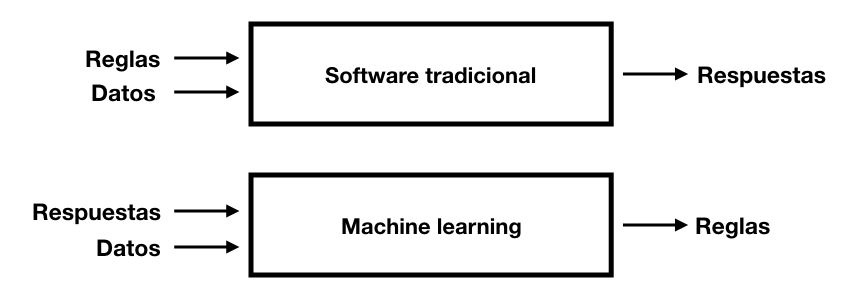
\includegraphics[width=0.85\textwidth,height=\textheight]{source/figures/tradicional.png}
\caption{Diferencias ente Software tradicional y Machine learning.
Elaboración propia. \label{tradicional}}
\end{figure}

Además, debido a la gran cantidad de información no estructurada
existente (imágenes, señales, textos, etc.) en medicina, como era de
esperar, el \textbf{Deep Learning} puede jugar un papel esencial,
permitiendo que los datos \emph{hablen por sí mismos}. Sin embargo, en
todo momento tenemos que tener presente que nuestras evaluaciones pueden
ser demasiado optimistas o que el sobreajuste puede hacer que nuestros
modelos dejen de funcionar al ponerlos en producción. Tener una
Inteligencia Artificial explicable, de la que no solo obtengamos
predicciones sino el por qué de las mismas, es algo que facilitará la
entrada de estos algoritmos en el día a día de los médicos.

A continuación se detallarán los ámbitos dentro del campo de la medicina
en la que el Aprendizaje Automático puede realizar importantes
contribuciones.

\hypertarget{pronuxf3stico}{%
\subsection{Pronóstico}\label{pronuxf3stico}}

El Machine Learning nos puede ayudar, mediante la búsqueda de patrones,
en la predicción de la evolución de un enfermo. En varios servicios de
salud existen ya implantados sistemas que, mediante Machine Learning,
son capaces de identificar a los pacientes que están en riesgo de tener
que ser transferidos a las unidades de cuidados intensivos. (Escobar
et~al. 2016). Además, diversos estudios sugieren que se pueden crear
eficaces modelos de pronóstico médico a partir de la información en
bruto de historiales (Rajkomar et~al. 2018) e imágenes médicas (De Fauw
et~al. 2018).

La estandarización de los historiales médicos electrónicos sería de gran
ayuda para la implantación de estos sistemas permitiendo, además, la
agregación de datos. Formatos como el \textbf{Fast Healthcare
Interoperability Resources (FHIR)} (Mandel et~al. 2016) han nacido en
los últimos años con este propósito.

\hypertarget{diagnuxf3stico}{%
\subsection{Diagnóstico}\label{diagnuxf3stico}}

Según concluye la Academia Nacional de Ciencias de EEUU, prácticamente
todos los pacientes serán diagnosticados de forma errónea al menos una
vez en su vida (Ball et~al. 2015). Diversos estudios han encontrado
problemas sistemáticos en los servicios de salud de todo el mundo. Hay
evidencias de que, en los sistemas en los que los servicios de
diagnóstico y tratamiento los realiza una misma organización obteniendo
mayores ingresos la compañía mediante la prescripción de medicamentos y
la solicitud de nuevas pruebas médicas, la tendencia a hacerlo aumenta
considerablemente (Currie et~al. 2014).

Los datos históricos pueden ser de gran ayuda para la identificación de
posibles patologías durante las visitas clínicas, encontrando patrones
complejos y ayudando a eliminar posibles errores y sesgos humanos. Los
modelos podrían, incluso, sugerir nuevas pruebas a los médicos en base a
los datos recogidos en tiempo real (Slack et~al. 1966).

\hypertarget{tratamiento}{%
\subsection{Tratamiento}\label{tratamiento}}

La aproximación más directa al problema del tratamiento mediante Machine
Learning sería la creación de modelos entrenados con datos históricos
que aprendieran los medicamentos recetados por los médicos en cada
situación. Sin embargo, esta aproximación tiene un claro problema, el
modelo aprendería los hábitos de prescripción de los médicos, que no
tienen por qué ser los ideales. Por lo tanto, en este campo aún más, es
de vital importancia generar datasets fiables y analizados en profundiad
por expertos para entrenar los modelos (Rajkomar et~al. 2019).

\hypertarget{retos-clave}{%
\subsection{Retos clave}\label{retos-clave}}

Uno de los principales retos en la creación de modelos de Aprendizaje
Automático para medicina es la \textbf{falta de datos de calidad}. Este
tipo de modelos, sobre todo los de Deep Learning, funcionan mejor cuanto
mayor es la cantidad de datos de los que disponen para su entrenamiento.
Sin embargo, en el campo de la medicina no existe tanta disponibilidad
de los mismos como sí que existe en otros ámbitos. Una de las
principales causas de esa escasez es la inviolable \textbf{privacidad}
de los datos de los pacientes, que a menudo impide la creación de
grandes datasets y únicamente permite crear conjuntos de datos lo
suficientemente agregados como para que no pueda obtenerse datos de una
persona en concreto. (Rajkomar et~al. 2019)

Otro de los retos es el \textbf{sesgo} existente en los datos. Toda
actividad humana está influenciada por un sesgo, ya sea consciente o
inconsciente. La máxima \textbf{Entrada basura/Salida basura} de la
analítica de datos está presente también en este campo. De nada servirá
contar con potentes modelos capaces de aprender complicados patrones, si
luego esos patrones los encontrará en datos erróneos o sesgados.

La \textbf{interpretabilidad} de los modelos es también clave. Los
médicos deben conocer el grado de veracidad y las limitaciones de estas
técnicas para poder incorporarlas como una herramienta más. La
sobreconfianza en estos sistemas puede conllevar una disminución de la
alerta de los médicos que puede tener consecuencias letales. Que los
modelos proporcionen, junto con sus predicciones, un grado de
confiabilidad es un buen principio, pero no basta. De hecho, en
ocasiones estos intervalos de fiabilidad pueden ser interpretados de
forma incorrecta (Jiang et~al. 2018). Es necesario crear modelos que
sean capaces de explicar el por qué de sus predicciones. De hecho, esto
era uno de los requisitos que indicó la Unión Europea en su \textbf{Guia
ética para una Inteligencia Artificial fiable}.\footnote{https://ec.europa.eu/digital-single-market/en/news/ethics-guidelines-trustworthy-ai}
La necesidad de interpretabilidad de los resultados pude suponer un
problema en técnicas de Deep Learning, que siempre han sido tachadas de
ser \textbf{cajas negras}. Sin embargo, en los últimos años se han
realizado diferentes estudios que demuestran que los modelos de Deep
Learning pueden ser interpretables con las herramientas adecuadas.
(Cruz-Roa et~al. 2013), (Lipton 2016), (Zhang \& Zhu 2018).

\hypertarget{correlaciuxf3n-no-implica-causalidad}{%
\section{Correlación no implica
causalidad}\label{correlaciuxf3n-no-implica-causalidad}}

Aunque sea un mantra repetido hasta la saciedad en la literatura, esta
advertencia merece un apartado propio en un trabajo de estas
características, pues es algo a tener en cuenta y que implica tener
mucha cautela al obtener conclusiones mediante este tipo de métodos. En
muchas ocasiones creemos, de forma errónea, que existe una relación de
causa y efecto entre dos variables que están correlacionadas, cuando
esto no siempre es cierto.

La correlación entre dos variables puede ser debida a una tercera
\textbf{variable oculta} que no tenemos por qué conocer o simplemente
puede ser lo que conocemos como \textbf{correlación espúrea}, es decir,
mera casualidad (que no causalidad).

Sin embargo, la falacia \textbf{Cum hoc ergo propter hoc} (en latín,
``Con esto, por tanto a causa de esto'') sigue siendo estando muy
presente en los medios de comunicación y en las \textbf{pseudociencias}.

Si alguna vez el lector divisa a un sujeto disfrazado de pirata, no lo
tome por loco. Ese sujeto podría ser un seguidor de \textbf{Bobby
Henderson}, creador de la iglesia pastafari que, cansado de argumentos
de los creacionistas basados en esta falacia, realizó un estudio (Figura
\ref{piratas}) en el que demostraba una clara correlación entre la
temperatura global y el descenso del número de piratas (un claro ejemplo
de la existencia de una variable oculta, el tiempo). Es común, desde
entonces, que los seguidores de Henderson se disfracen de piratas para
recordarlo.

\begin{figure}
\centering
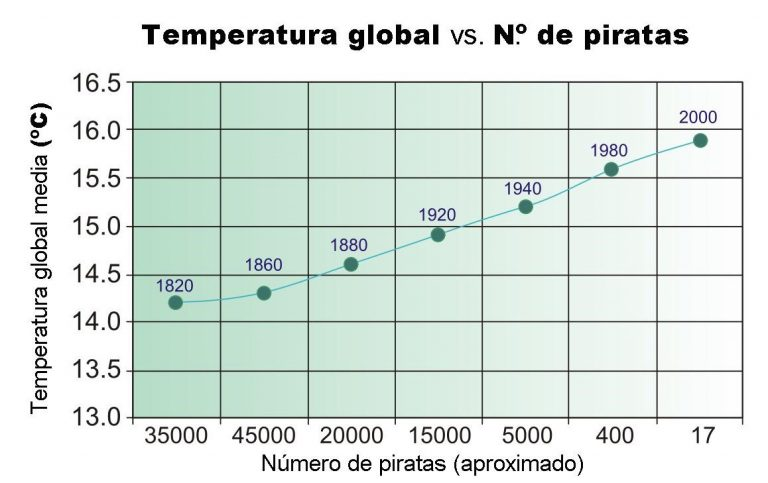
\includegraphics[width=0.9\textwidth,height=\textheight]{source/figures/piratas.jpg}
\caption{Correlación entre el aumento de la temperatura media global y
el descenso del número de piratas. Fuente:
https://www.jotdown.es/2016/06/correlacion-no-implica-causalidad/
\label{piratas}}
\end{figure}

Otro ejemplo curioso es la singular correlación entre el número de
ahogados en piscinas en Estados Unidos y el número de apariciones en
películas de Nicholas Cage (Figura \ref{cage}), en este caso una clara
correlación espúrea. Si se torturan los datos durante el tiempo
suficiente, éstos confesarán lo que deseemos.

\begin{figure}
\centering
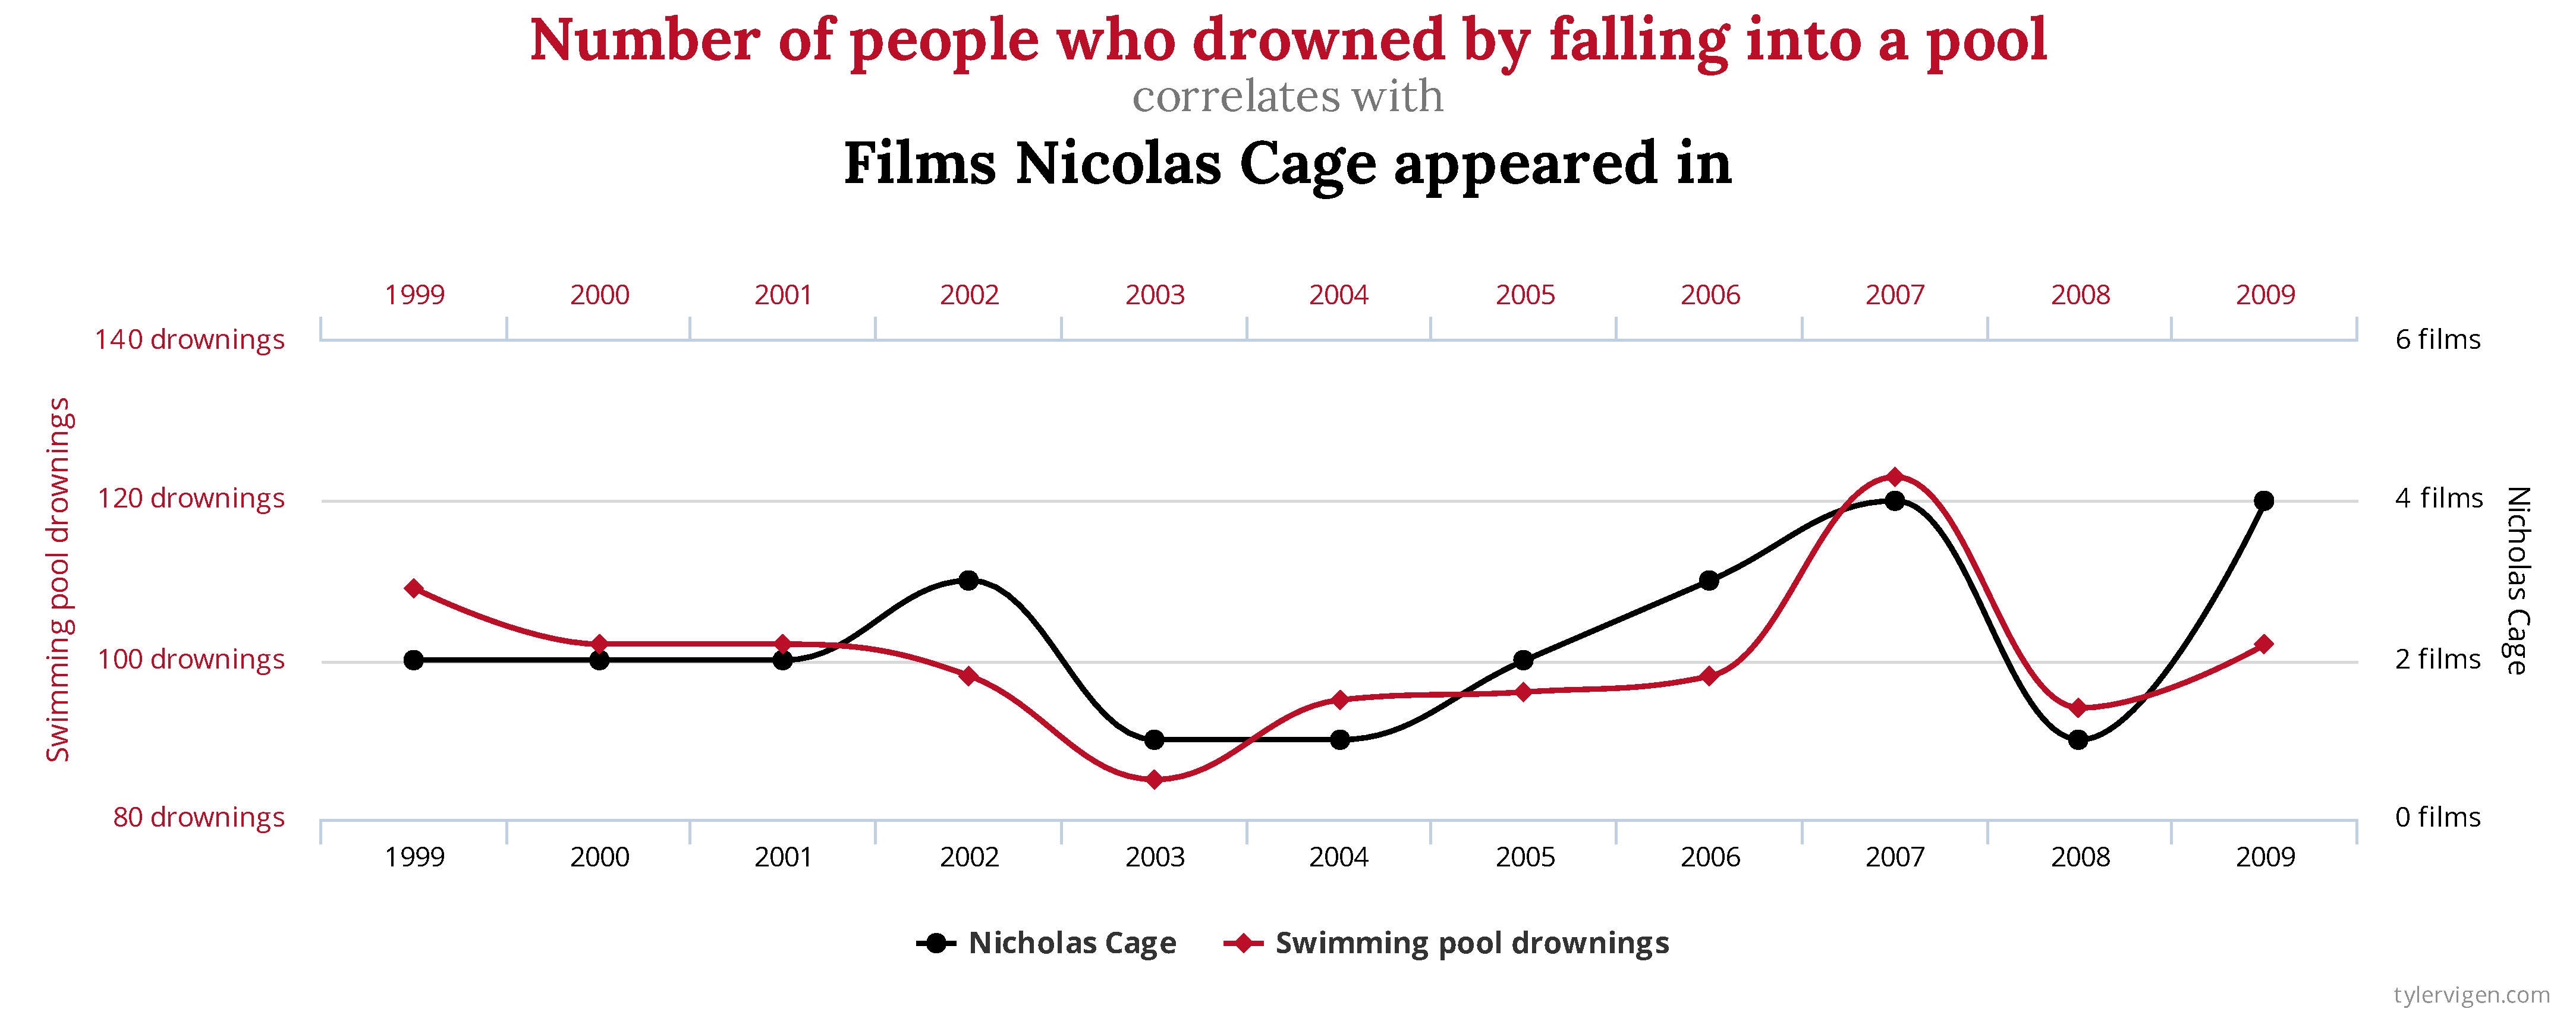
\includegraphics[width=1\textwidth,height=\textheight]{source/figures/cage.pdf}
\caption{Correlación entre el número de ahogados en piscinas de Estados
Unidos y el número de apariciones en películas de Nicholas Cage. Fuente:
http://www.tylervigen.com/spurious-correlations \label{cage}}
\end{figure}

Sin embargo, lejos de quedar en una mera anécdota como las anteriores,
es extremadamente preocupante que existan familias en todo el mundo que
estén decidiendo no vacunar a sus hijos debido a una aparente
correlación, en un estudio de 2010, entre el número de casos de autismo
y las vacunaciones.

Por lo tanto, es necesaria una gran cautela antes de obtener
conclusiones de los sistemas de Machine Learning. Además, no estaría de
más, aunque no serán objeto de análisis en este trabajo, tener presentes
el Sesgo del Superviviente\footnote{https://es.wikipedia.org/wiki/Sesgo\_del\_superviviente}
y la Paradoja de Simpson\footnote{https://es.wikipedia.org/wiki/Paradoja\_de\_Simpson}).

\hypertarget{arte}{%
\chapter{Estado del arte en detección de RD y DMAE}\label{arte}}

A lo largo de este capítulo se analizará el estado del arte de la
detección de \textbf{Retinopatía Diabética} y \textbf{Degeneración
Macular Asociada a la Edad} a partir de imágenes de fondo de ojo. En la
actualidad, prácticamente la totalidad de los nuevos modelos publicados
en este campo son modelos de \textbf{Deep Learning}. Sin embargo, se
comenzará analizando los modelos basados en \textbf{Machine Learning}
que precedieron a los actuales.

Al no existir en este campo un conjunto de datos de referencia sobre el
que se evalúen todos los modelos, hay que tomar con cierta cautela las
métricas de evaluación de los algoritmos que se detallarán a lo largo de
este capítulo, puesto que cada modelo habrá sido entrenado y evaluado
con datos distintos. De hecho, muchos de estos modelos han sido
entrenados con conjuntos de apenas 100 o 200 imágenes, lo que hace muy
probable que exista \textbf{sobreajuste} (u \emph{overfitting}) y que el
resultado de ponerlos en producción sea mucho peor del esperado.

\hypertarget{aproximaciones-basadas-en-machine-learning}{%
\section{Aproximaciones basadas en Machine
Learning}\label{aproximaciones-basadas-en-machine-learning}}

Las modelos basados en Machine Learning para la detección de patologías
en imágenes de fondo de ojo requieren una gran cantidad de
\textbf{características}, escogidas y extraídas, de cada imagen, de
forma manual por los investigadores. Para la obtención de las mismas es
necesario \textbf{conocimiento experto} en la materia. Además, este tipo
de características tienden a no generalizar bien, dando lugar a modelos,
en muchas ocasiones, sobreajustados. Sin embargo, en los casos en los
que nuestro conjunto de imágenes de entrenamiento es muy limitado, es
común que los modelos basados en Machine Learning nos ofrezcan mejores
resultados que los basados en Deep Learning. Además, la
interpretabilidad de los modelos finales y sus predicciones es mayor en
los modelos de Machine Learning que en los de Deep Learning.

\hypertarget{detecciuxf3n-de-rd-mediante-machine-learning}{%
\subsection{Detección de RD mediante Machine
Learning}\label{detecciuxf3n-de-rd-mediante-machine-learning}}

Este tipo técnicas se basan en la búsqueda, en las imágenes, de cada una
de las lesiones que caracterizan la Retinopatía Diabética. Las lesiones
que caracterizan la RD, como se ha analizado anteriormente, son:
\textbf{exudados}, \textbf{microaneurismas} y \textbf{hemorragias}. En
el caso de la PDR, es posible encontrar también
\textbf{neovascularización}. A partir de características obtenidas
principalmente mediante técnicas de procesamiento digital de imágen y
gracias al uso de \textbf{clasificadores basados en Machine Learning} es
posible detectar la enfermedad, e incluso, estimar su gravedad.

Muchos de estos modelos comienzan por la obtención de imágenes binarias
que representaran los \textbf{vasos sanguíneos} presentes en la imagen
de la retina (Figura \ref{venas}). La longitud, tamaño o posición de los
mismos son de gran ayuda para el diagnóstico de la RD. Mediante la
aplicación de una serie de técnicas al canal verde de las imágenes de
fondo de ojo, es posible aislar estos vasos del resto de la imagen
(Acharya et~al. 2009). Otros modelos se basan también en la detección y
seguimiento de las líneas centrales de los vasos sanguíneos (Tolias \&
Panas 1998) (Englmeier et~al. 2004) (Vlachos \& Dermatas 2010). También
existen técnicas más avanzadas para ello basadas en el uso de
\textbf{filtros adaptados} de dos dimensiones (Katz et~al. 1989) (Hoover
et~al. 1998) (Mookiah, U Rajendra Acharya, Martis, et~al. 2013) (Gang
et~al. 2002). A partir de estos pre-procesamientos, existen sistemas
capaces de detectar anchuras anormales en estos vasos sanguíneos
(Hayashi et~al. 2001), que suelen ser un indicio de la existencia de RD.

\begin{figure}
\centering
\includegraphics[width=0.9\textwidth,height=\textheight]{source/figures/venas.tif}
\caption{Imagen binaria de los vasos sanguíneos de la retina. Fuente:
http://www.aria-database.com/ \label{venas}}
\end{figure}

La presencia de \textbf{hemorragias} en las imágenes de fondo de ojo es
mayor en los estadios más graves de la enfermedad. Su detección se
realiza habitualmente junto con la detección de los vasos sanguíneos.

La presencia de \textbf{exudados} es el síntoma más característico de
RD. Para la detección de éstos es común comenzar por la eliminación de
los vasos sanguíneos y el disco óptico de las imágenes. Una vez
eliminados estos elementos, es posible detectar los exudados mediante
una secuencia de algoritmos de procesamiento de imágen (Acharya et~al.
2009). Técnicas más avanzadas, basadas en \textbf{clasificadores
estadísticos} basados en los niveles de brillo y uso de ventanas
espaciales como estrategia de verificación han obtenido resultados
cercanos all 100\% de exactitud en la detección de imágenes con exudados
(sensibilidad) y 70\% de exactitud en la detección de imágenes de
retinas sanas (especificidad) (Wang et~al. 2000). Técnicas de detección
de exudados basadas en \textbf{redes neuronales} (Hunter et~al. 2000) o
en el algoritmo \textbf{PCA}\footnote{Principal Components Analysis} (Li
\& Chutatape 2000) también han conseguido resultados similares a los
comentados anteriormente. Esta última técnica, también permitía obtener
la localización del disco óptico y la fóvea con unas exactitudes,
respectivamente, de 99\% y 100\%.

A partir de la presencia de \textbf{microaneurismas} es también posibe
la detección de la RD, llegando a conseguirse una sensibilidad del 85\%
y una especificidad del 90\% (Jelinek et~al. 2006). La forma de
detectarlos es similar a las anteriores y requiere eliminar el disco
óptico y los vasos sanguíneos de la imagen antes de aplicar una serie de
técnicas de procesamiento de imágenes. También es posible el uso de
técnicas basadas en \textbf{morfología matemática} (Walter et~al. 2007)
(Hatanaka et~al. 2008). Algunos de estos métodos realizan
\textbf{transformaciones del espacio de color} de las imágenes a HSV
(Hue, Saturation, Value), espacio donde les es más fácil realizar el
procesamiento. El uso de las \textbf{transformada Wavelet} también ha
demostrado ser eficaz en la detección de microaneurismas (Quellec et~al.
2008).

De la misma forma que muchas de las técnicas explicadas hasta ahora
basan su predicción en la detección de alguna de las lesiones típicas de
la RD, también existen sistemas más complejos que son capaces de
detectar, de forma simultánea, los tres tipos de lesiones y realizar
predicciones en base a la presencia de cada tipo de lesión mediante
clasificadores como \textbf{árboles de decisión} o \textbf{redes
neuronales} (Ege et~al. 2000), (Sinthanayothin et~al. 2002),
(Sinthanayothin et~al. 2003), (Reza \& Eswaran 2011). Técnicas de
aprendizaje no supervisado como el \textbf{FCM}\footnote{Fuzzy c-means}
también han demostrado ser eficaces en esta tarea (Osareh et~al. 2002)

Todas las investigaciones analizadas anteriormente trataban de predecir
una variable binaria, la presencia o no de retinopatía diabética. Sin
embargo, otras investigaciones han tratado de detectar también el
\textbf{tipo de RD} (Proliferativa o No Proliferativa). Estas técnicas
han conseguido sensibilidad y especifidad de más del 95\% (Mookiah, U
Rajendra Acharya, Martis, et~al. 2013) mediante el uso de \textbf{redes
neuronales}. Otros trabajos han intentado distinguir, con éxito, hasta
\textbf{5 grados de RD} (Acharya et~al. 2008),(Acharya et~al. 2009),
(Acharya et~al. 2012).

\hypertarget{detecciuxf3n-de-dmae-mediante-machine-learning}{%
\subsection{Detección de DMAE mediante Machine
Learning}\label{detecciuxf3n-de-dmae-mediante-machine-learning}}

A pesar de ser la mayor causa de ceguera en países desarrollados (Wong
et~al. 2014), la detección de la \textbf{Degeneración Macular Asociada a
la Edad (DMAE)} en imágenes de fondo de ojo no ha despertado tanto
interés en la comunidad científica como la Retinopatía Diabética. Una
extensa búsqueda en la bibliografía arroja un solo estudio (Pead et~al.
2019) que analiza todos los métodos actuales de detección de DMAE
basados en Machine Learning y Deep Learning. Ese estudio concluye que
únicamente existen 14 publicaciones que abordan este tema.\footnote{La
  búsqueda realizada filtra las publicaciones que no contengan una
  evaluación robusta del modelo, que no estén escritas en inglés o que
  no utilicen un método basado en las imágenes de fondo de ojo}

El principal signo de DMAE, como se ha analizado en capítulos
anteriores, es la aparición de \textbf{drusas}, que pueden ser
observadas en la imágenes de fondo de ojo como pequeños conjuntos de
manchas blancas y amarillas. Por lo tanto, este tipo de modelos tratarán
de buscar estas lesiones en las imágenes. En la Figura \ref{metodosamd}
vemos cuáles son las tareas principales en la detección de DMAE mediante
Machine Learning.

\begin{figure}
\centering
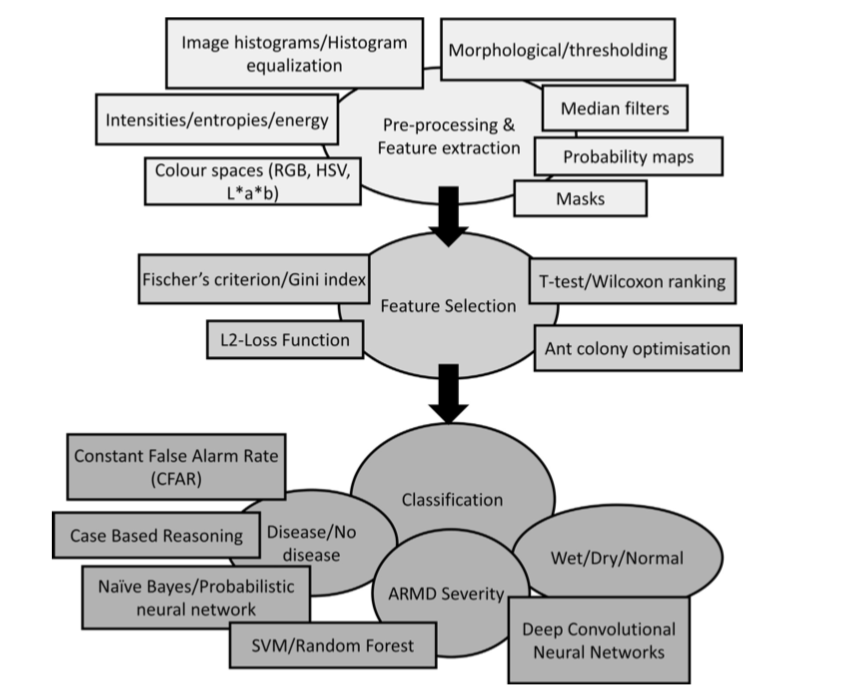
\includegraphics[width=0.9\textwidth,height=\textheight]{source/figures/fases-amd.png}
\caption{Resumen de las fases de la detección de DMAE mediante Machine
Learning. Fuente: (Pead et~al. 2019) \label{metodosamd}}
\end{figure}

Como se ha explicado en el anterior apartado, los algoritmos basados en
Machine Learning suelen requerir de una fase de \textbf{pre-procesado y
extracción de características}, dado que no son capaces de procesar la
imágen \emph{en bruto}. Puesto que las drusas son pequeñas regiones
brillantes en las imágenes, algunos métodos han utilizado para su
detección diversas características calculadas a partir de los
\textbf{histogramas} de las imágenes. Además, es común aplicar una
\textbf{ecualización del histograma} como paso previo a la extracción de
características para obtener un mayor contraste en las imágenes (Hijazi
et~al. 2010), (Yalin Zheng et~al. 2012), (Mookiah, U Rajendra Acharya,
Koh, Chandran, et~al. 2014), (Mookiah, U Rajendra Acharya, Koh, Chua,
et~al. 2014). Aplicar un \textbf{filtro de mediana} permite eliminar,
antes de la extracción de características, el ruido de alta frecuencia
de las imágenes (Kankanahalli et~al. 2013) (Phan et~al. 2016). El uso de
técnicas de \textbf{morfología matemática} también ha demostrado ser
eficaz para resaltar las regiones con drusas de la imagen (Burlina
et~al. 2011), (Garcı́a-Floriano et~al. 2017).

Tras el \textbf{pre-procesado y extracción de características} es común
realizar una \textbf{selección de características} que nos permite
eliminar características (o columnas o campos) que puedan resultar
irrelevantes o puedan confundir a los algoritmos de Machine Learning.
Para esto, se han utilizado algoritmos basados en la \textbf{correlación
entre las distintas características} (Garcı́a-Floriano et~al. 2017) test
paramétricos y no paramétricos como el \textbf{t-test} (Mookiah, U
Rajendra Acharya, Koh, Chandran, et~al. 2014), (Mookiah, U Rajendra
Acharya, Koh, Chua, et~al. 2014) o, incluso, \textbf{algoritmos
genéticos} (Acharya et~al. 2017)

En el último paso, la \textbf{clasificación}, podemos separar los
algoritmos en dos grupos: los que simplemente tratan de diferenciar
entre sano/enfermo y los que tratan también de detectar grados de
afectación de la enfermedad. Dentro del primer grupo encontramos métodos
como el \textbf{Razonamiento Basado en Casos} en el que, de forma
similar al algoritmo \textbf{K-Nearest Neighbors}, simplemente se mide
el grado de parecido entre el histograma de la imágen de fondo de ojo a
predecir y cada uno de los histogramas de las imágenes del conjunto de
datos de entrenamiento (Hijazi et~al. 2010). También encontramos métodos
basados en los algoritmos \textbf{Naive Bayes} o \textbf{SVM} (Zheng
et~al. 2011), (Garcı́a-Floriano et~al. 2017). Sin embargo, otras
publicaciones han tratado de detectar también la gravedad de la
enfermedad (estableciendo 5 posibles grados) con algoritmos como
\textbf{Random Forest}, \textbf{K-Nearest Neighbors} o \textbf{SVM}
(Kankanahalli et~al. 2013), (Phan et~al. 2016).

\hypertarget{aproximaciones-basadas-en-deep-learning}{%
\section{Aproximaciones basadas en Deep
Learning}\label{aproximaciones-basadas-en-deep-learning}}

Las aproximaciones basadas en \textbf{Deep Learning}, haciendo uso de
\textbf{Redes Neuronales Convolucionales}, representan actualmente el
estado del arte en multitud de tareas de análisis de imágenes médicas.
Entre ellas se encuentra también, como no podía ser de otra forma, el
análisis de imágenes de fondo de ojo. Una de las principales ventajas de
este tipo de aproximaciones es que se elimina la necesidad de la
extracción de características en base a conocimiento experto. De esta
forma, \textbf{la red es directamente alimentada con las imágenes},
siendo tarea de ésta la extracción de características que permitan
distinguir con eficacia las distintas clases de nuestro problema.

\hypertarget{detecciuxf3n-de-rd-mediante-deep-learning}{%
\subsection{Detección de RD mediante Deep
Learning}\label{detecciuxf3n-de-rd-mediante-deep-learning}}

Existen dos grupos principales de algoritmos de Deep Learning para la
detección de Retinopatía Diabética: los que tratan de detectar y
localizar en la imagen de fondo de ojo cada una de las lesiones típicas
de la RD y los que, por el contrario, tratan de detectar directamente la
presencia de la enfermedad sin enfocarse en detectar ni localizar las
lesiones concretas. Es este segundo grupo el que nos interesa analizar,
pues es la metodología que utilizaremos en la creación de nuestro
modelo. Además, la gran ventaja de este tipo de modelos es que no
necesita un dataset con anotaciones de la localización de las lesiones
para ser entrenados. Simplemente necesitamos un conjunto de datos con
etiquetas de \textbf{sano/enfermo}.

Prácticamente todos los modelos de este tipo han sido \textbf{Redes
Neuronales Convolucionales}. La arquitectura \textbf{Inception} ha
demostrado ser muy efectiva en la detección de la RD proliferativa.
(Gulshan et~al. 2016). En este caso, se trataba de una clasificación
binaria donde sólo existían dos posibles salidas (enfermo/sano). Sin
embargo, muchos otros investigadores han tratado de detectar diferentes
niveles de gravedad (Colas et~al. 2016), (Quellec et~al. 2017), (Costa
\& Campilho 2017). Además, agunos de estos modelos son capaces de
detectar también las lesiones concretas que aparecen en cada imagen
(Colas et~al. 2016), (Quellec et~al. 2017)

Otros investigadores también han hecho uso, de forma satisfactoria, de
la arquitectura \textbf{AlexNet} (Mansour 2018), o \textbf{ResNet}
(Gargeya \& Leng 2017). Además, este último modelo añadía al final de la
red una capa convolucional adicional que permitía observar e interpretar
el proceso de aprendizaje de la red, solventando así el problema de
interpretabilidad que a menudo tienen este tipo de modelos. La gran
interpretabilidad, junto con una alta \textbf{accuracy} hacen que este
modelo sea para muchos investigadores el \textbf{modelo de referencia}
en detección de Retinopatía Diabética.

También se han realizado investigaciones con pasos previos de extracción
de características usando técnicas como \textbf{Bag Of Visual Words}
(Costa \& Campilho 2017) o extracción del fondo de las imágenes mediante
\textbf{Modelos Gaussianos Mixtos} (Mansour 2018)

Otras técnicas, como la de \textbf{Data Augmentation} consistente en
crear nuevas imágenes a partir de transformaciones sobre las imágenes
originales, han demostrado también ser eficaces (Pratt et~al. 2016).

Además del Data Augmentation, otra técnica que también ha sido usada
para solventar el problema de la falta de imágenes ha sido el
\textbf{Transfer Learning}. Esta técnica ha sido aplicada utilizando,
como base para nuestros modelos, otros modelos que habían sido
previamente entrenados en otros datasets con todo tipo de imágenes
(Maninis et~al. 2016), (Li et~al. 2017) o con datasets específicos de
imágenes de fondo de ojo (Gondal et~al. 2017). De ambas formas ha
demostrado ser de utilidad, especialmente en los casos en los que el
conjunto de imágenes de entrenamiento era demasiado reducido como para
poder entrenar una arquitectura compleja desde cero.

\hypertarget{detecciuxf3n-de-dmae-mediante-deep-learning}{%
\subsection{Detección de DMAE mediante Deep
Learning}\label{detecciuxf3n-de-dmae-mediante-deep-learning}}

De la misma forma que con la Retinopatía Diabética, los métodos de
detección de DMAE basados en Deep Learning han permitido saltar la etapa
de extracción de características, delegándola en el propio clasificador.
Prácticamente la totalidad de los modelos de Deep Learning de este tipo
han hecho uso de \textbf{Redes Neuronales Convolucionales}. Estas redes
han sido entrenadas desde 0 (Tan et~al. 2018) o, en ocasiones se ha
hecho uso de la técnica del \textbf{Transfer Learning}. Gracias a ésta,
se han utilizado los pesos de redes entrenadas previamente en otros
conjuntos de imágenes como punto de partida para el entrenamiento de las
últimas capas de las redes convolucionales (Burlina et~al. 2016).
Además, como es común en Deep Learning, también se han propuesto algunos
modelos basados en la combinación de las predicciones de varios modelos
distintos (Grassmann et~al. 2018), técnica conocida como
\textbf{ensemble}. Sin embargo, la cantidad de publicaciones que abordan
la detección de DMAE mediante Deep Learning es aún muy limitada y es de
esperar que muchas de las técnicas avanzadas que ya se están utilizando
en la detección de Retinopatía Diabética sean aplicadas durante los
próximos años a la detección del a Degeneración Macular Asociada a la
Edad.

\hypertarget{sistema}{%
\chapter{Diseño de Sistema de Detección de RD y DMAE}\label{sistema}}

La \textbf{gran cantidad de conjuntos de imágenes} utilizados y el
\textbf{extremo desbalanceo} de las clases han sido los dos factores que
más han condicionado el diseño de los sistemas. Esto ha provocado que se
hayan realizado \textbf{3 aproximaciones distintas al problema}, todas
ellas basadas en Deep Learning, y únicamente obteniendo resultados
útiles de 2 de ellas.

Durante este capítulo se analizarán estas aproximaciones. Este análisis
no se limitará a una simple descripción del clasificador utilizado, sino
que se detallarán los principales aspectos de cualquier proyecto de este
tipo: los \textbf{datos} usados, su limpieza y procesado, el proceso de
selección de \textbf{hiperparámetros} o incluso las características y
limitaciones impuestas por los \textbf{recursos hardware y software}
utilizados.

\hypertarget{exploraciuxf3n-de-los-datos}{%
\section{Exploración de los datos}\label{exploraciuxf3n-de-los-datos}}

Una de las principales contribuciones de esta investigación ha sido
precisamente la \textbf{extensa cantidad de conjuntos distintos de
imágenes} utilizados en la creación de los modelos. Para entrenar el
modelo se han seleccionado imágenes de prácticamente todos los datasets
utilizados por los sistemas del capítulo \ref{arte}. En total han sido
utilizados \textbf{13 conjuntos de imágenes}, con un total de
\textbf{39118 imágenes}.\footnote{Sin embargo, como se verá durante este
  capítulo, algunos de los clasificadores que se han entrenado no han
  utilizado el conjunto completo de imágenes para el entrenamiento.}
Destaca el dataset \textbf{Kaggle} que contiene el 66\% del total de
imágenes utilizadas. Este dataset proviene de una competición\footnote{https://www.kaggle.com/c/diabetic-retinopathy-detection/}
realizada en 2015 que supuso importantes avances en la detección de
Retinopatía Diabética a partir de imágenes de fondo de ojo.

Como se ha visto, la cantidad total de imágenes es muy elevada, siendo
muy superior al tamaño medio de los datasets de los modelos analizados
en el capítulo \ref{arte}. Algunos de los modelos creados han utilizado
grupos más reducidos de imágenes, seleccionadas aleatoriamente del
conjunto de datos original. En la tabla \ref{datasets0} se muestra la
cantidad de imágenes de cada tipo existentes en cada uno de los datasets
utilizados.

\begin{longtable}[]{@{}lccc@{}}
\caption{Cantidad de imágenes de cada tipo en cada uno de los conjuntos
de imágenes utilizados \label{datasets0}}\tabularnewline
\toprule
\begin{minipage}[b]{0.35\columnwidth}\raggedright
Dataset\strut
\end{minipage} & \begin{minipage}[b]{0.19\columnwidth}\centering
SANA\strut
\end{minipage} & \begin{minipage}[b]{0.17\columnwidth}\centering
RD\strut
\end{minipage} & \begin{minipage}[b]{0.17\columnwidth}\centering
DMAE\strut
\end{minipage}\tabularnewline
\midrule
\endfirsthead
\toprule
\begin{minipage}[b]{0.35\columnwidth}\raggedright
Dataset\strut
\end{minipage} & \begin{minipage}[b]{0.19\columnwidth}\centering
SANA\strut
\end{minipage} & \begin{minipage}[b]{0.17\columnwidth}\centering
RD\strut
\end{minipage} & \begin{minipage}[b]{0.17\columnwidth}\centering
DMAE\strut
\end{minipage}\tabularnewline
\midrule
\endhead
\begin{minipage}[t]{0.35\columnwidth}\raggedright
GRAND-CHALLENGE\strut
\end{minipage} & \begin{minipage}[t]{0.19\columnwidth}\centering
311\strut
\end{minipage} & \begin{minipage}[t]{0.17\columnwidth}\centering
0\strut
\end{minipage} & \begin{minipage}[t]{0.17\columnwidth}\centering
89\strut
\end{minipage}\tabularnewline
\begin{minipage}[t]{0.35\columnwidth}\raggedright
ARIA\strut
\end{minipage} & \begin{minipage}[t]{0.19\columnwidth}\centering
61\strut
\end{minipage} & \begin{minipage}[t]{0.17\columnwidth}\centering
59\strut
\end{minipage} & \begin{minipage}[t]{0.17\columnwidth}\centering
23\strut
\end{minipage}\tabularnewline
\begin{minipage}[t]{0.35\columnwidth}\raggedright
DIARET DB0\strut
\end{minipage} & \begin{minipage}[t]{0.19\columnwidth}\centering
20\strut
\end{minipage} & \begin{minipage}[t]{0.17\columnwidth}\centering
110\strut
\end{minipage} & \begin{minipage}[t]{0.17\columnwidth}\centering
0\strut
\end{minipage}\tabularnewline
\begin{minipage}[t]{0.35\columnwidth}\raggedright
E-OPTHA\strut
\end{minipage} & \begin{minipage}[t]{0.19\columnwidth}\centering
268\strut
\end{minipage} & \begin{minipage}[t]{0.17\columnwidth}\centering
195\strut
\end{minipage} & \begin{minipage}[t]{0.17\columnwidth}\centering
0\strut
\end{minipage}\tabularnewline
\begin{minipage}[t]{0.35\columnwidth}\raggedright
HEI-MED\strut
\end{minipage} & \begin{minipage}[t]{0.19\columnwidth}\centering
0\strut
\end{minipage} & \begin{minipage}[t]{0.17\columnwidth}\centering
169\strut
\end{minipage} & \begin{minipage}[t]{0.17\columnwidth}\centering
0\strut
\end{minipage}\tabularnewline
\begin{minipage}[t]{0.35\columnwidth}\raggedright
HRF\strut
\end{minipage} & \begin{minipage}[t]{0.19\columnwidth}\centering
15\strut
\end{minipage} & \begin{minipage}[t]{0.17\columnwidth}\centering
15\strut
\end{minipage} & \begin{minipage}[t]{0.17\columnwidth}\centering
0\strut
\end{minipage}\tabularnewline
\begin{minipage}[t]{0.35\columnwidth}\raggedright
KAGGLE\strut
\end{minipage} & \begin{minipage}[t]{0.19\columnwidth}\centering
25810\strut
\end{minipage} & \begin{minipage}[t]{0.17\columnwidth}\centering
9316\strut
\end{minipage} & \begin{minipage}[t]{0.17\columnwidth}\centering
0\strut
\end{minipage}\tabularnewline
\begin{minipage}[t]{0.35\columnwidth}\raggedright
MESSIDOR\strut
\end{minipage} & \begin{minipage}[t]{0.19\columnwidth}\centering
540\strut
\end{minipage} & \begin{minipage}[t]{0.17\columnwidth}\centering
660\strut
\end{minipage} & \begin{minipage}[t]{0.17\columnwidth}\centering
0\strut
\end{minipage}\tabularnewline
\begin{minipage}[t]{0.35\columnwidth}\raggedright
ONHSD\strut
\end{minipage} & \begin{minipage}[t]{0.19\columnwidth}\centering
0\strut
\end{minipage} & \begin{minipage}[t]{0.17\columnwidth}\centering
99\strut
\end{minipage} & \begin{minipage}[t]{0.17\columnwidth}\centering
0\strut
\end{minipage}\tabularnewline
\begin{minipage}[t]{0.35\columnwidth}\raggedright
ROC\strut
\end{minipage} & \begin{minipage}[t]{0.19\columnwidth}\centering
0\strut
\end{minipage} & \begin{minipage}[t]{0.17\columnwidth}\centering
50\strut
\end{minipage} & \begin{minipage}[t]{0.17\columnwidth}\centering
0\strut
\end{minipage}\tabularnewline
\begin{minipage}[t]{0.35\columnwidth}\raggedright
DIAGNOS\strut
\end{minipage} & \begin{minipage}[t]{0.19\columnwidth}\centering
23\strut
\end{minipage} & \begin{minipage}[t]{0.17\columnwidth}\centering
0\strut
\end{minipage} & \begin{minipage}[t]{0.17\columnwidth}\centering
22\strut
\end{minipage}\tabularnewline
\begin{minipage}[t]{0.35\columnwidth}\raggedright
STARE\strut
\end{minipage} & \begin{minipage}[t]{0.19\columnwidth}\centering
37\strut
\end{minipage} & \begin{minipage}[t]{0.17\columnwidth}\centering
89\strut
\end{minipage} & \begin{minipage}[t]{0.17\columnwidth}\centering
47\strut
\end{minipage}\tabularnewline
\begin{minipage}[t]{0.35\columnwidth}\raggedright
FOM\strut
\end{minipage} & \begin{minipage}[t]{0.19\columnwidth}\centering
533\strut
\end{minipage} & \begin{minipage}[t]{0.17\columnwidth}\centering
457\strut
\end{minipage} & \begin{minipage}[t]{0.17\columnwidth}\centering
101\strut
\end{minipage}\tabularnewline
\bottomrule
\end{longtable}

Haber utilizado todos estos datasets ha supuesto una dificultad añadida
al proceso pues se ha tenido que realizar un costoso trabajo previo de
\textbf{selección, limpieza y preparación de los datos}. Se han creado
una serie de scripts que han recorrido cada una de las carpetas y han
separado las imágenes de cada tipo.

Como se puede observar en los datos de la tabla \ref{datasets1}, el gran
problema del conjunto de imágenes utilizado, que ha condicionado en gran
medida la forma de trabajar con él, es el gran \textbf{desbalanceo}
existente entre las clases. La clase predominante, las imágenes de
retinas sanas, contiene \textbf{más del 70\%} del total de imágenes. Por
el contrario la clase minoritaria, las imágenes de retinas con DMAE,
únicamente contiene 281 imágenes, \textbf{menos del 1\% del total}. Este
gran desbalanceo nos obligará a aplicar diversas técnicas que permitan
compensarlo como la \textbf{asignación de pesos distintos a las
instancias de cada clase} en el cálculo de la función de coste o el
\textbf{submuestreo de los datasets}.

\begin{longtable}[]{@{}ccc@{}}
\caption{Cantidad de imágenes de cada tipo en el conjunto completo de
datos utilizado \label{datasets1}}\tabularnewline
\toprule
\begin{minipage}[b]{0.28\columnwidth}\centering
Clase\strut
\end{minipage} & \begin{minipage}[b]{0.32\columnwidth}\centering
Total de imágenes\strut
\end{minipage} & \begin{minipage}[b]{0.32\columnwidth}\centering
\% del dataset completo\strut
\end{minipage}\tabularnewline
\midrule
\endfirsthead
\toprule
\begin{minipage}[b]{0.28\columnwidth}\centering
Clase\strut
\end{minipage} & \begin{minipage}[b]{0.32\columnwidth}\centering
Total de imágenes\strut
\end{minipage} & \begin{minipage}[b]{0.32\columnwidth}\centering
\% del dataset completo\strut
\end{minipage}\tabularnewline
\midrule
\endhead
\begin{minipage}[t]{0.28\columnwidth}\centering
Todas\strut
\end{minipage} & \begin{minipage}[t]{0.32\columnwidth}\centering
39118\strut
\end{minipage} & \begin{minipage}[t]{0.32\columnwidth}\centering
100\strut
\end{minipage}\tabularnewline
\begin{minipage}[t]{0.28\columnwidth}\centering
Sanas\strut
\end{minipage} & \begin{minipage}[t]{0.32\columnwidth}\centering
27618\strut
\end{minipage} & \begin{minipage}[t]{0.32\columnwidth}\centering
70.60\strut
\end{minipage}\tabularnewline
\begin{minipage}[t]{0.28\columnwidth}\centering
RD\strut
\end{minipage} & \begin{minipage}[t]{0.32\columnwidth}\centering
11219\strut
\end{minipage} & \begin{minipage}[t]{0.32\columnwidth}\centering
28.68\strut
\end{minipage}\tabularnewline
\begin{minipage}[t]{0.28\columnwidth}\centering
DMAE\strut
\end{minipage} & \begin{minipage}[t]{0.32\columnwidth}\centering
281\strut
\end{minipage} & \begin{minipage}[t]{0.32\columnwidth}\centering
0.72\strut
\end{minipage}\tabularnewline
\bottomrule
\end{longtable}

Otra dificultad derivada del uso de 13 datasets distintos es que nuestro
clasificador tendrá que tratar imágenes con características muy
distintas, como se observa en la tabla \ref{datasets2}. Las condiciones
en las que han sido tomadas, procesadas y almacenadas las imágenes
varían en gran medida entre los distintos datasets. Sin embargo, si se
pretende crear un clasificador robusto que sea capaz de trabajar en todo
tipo de condiciones, utilizar esta elevada cantidad de conjuntos de
imágenes será de gran ayuda.

\newpage

\begin{longtable}[]{@{}cccc@{}}
\caption{Características de las imágenes de cada uno de los conjuntos
utilizados \label{datasets2}}\tabularnewline
\toprule
\begin{minipage}[b]{0.33\columnwidth}\centering
Dataset\strut
\end{minipage} & \begin{minipage}[b]{0.33\columnwidth}\centering
Origen\strut
\end{minipage} & \begin{minipage}[b]{0.13\columnwidth}\centering
Tamaño\strut
\end{minipage} & \begin{minipage}[b]{0.09\columnwidth}\centering
Formato\strut
\end{minipage}\tabularnewline
\midrule
\endfirsthead
\toprule
\begin{minipage}[b]{0.33\columnwidth}\centering
Dataset\strut
\end{minipage} & \begin{minipage}[b]{0.33\columnwidth}\centering
Origen\strut
\end{minipage} & \begin{minipage}[b]{0.13\columnwidth}\centering
Tamaño\strut
\end{minipage} & \begin{minipage}[b]{0.09\columnwidth}\centering
Formato\strut
\end{minipage}\tabularnewline
\midrule
\endhead
\begin{minipage}[t]{0.33\columnwidth}\centering
GRAND-CHALLENGE\strut
\end{minipage} & \begin{minipage}[t]{0.33\columnwidth}\centering
(Anón s.~f.)\strut
\end{minipage} & \begin{minipage}[t]{0.13\columnwidth}\centering
Varios\strut
\end{minipage} & \begin{minipage}[t]{0.09\columnwidth}\centering
JPG\strut
\end{minipage}\tabularnewline
\begin{minipage}[t]{0.33\columnwidth}\centering
ARIA\strut
\end{minipage} & \begin{minipage}[t]{0.33\columnwidth}\centering
(Yalin Zheng et~al. 2012) (Farnell et~al. 2008)\strut
\end{minipage} & \begin{minipage}[t]{0.13\columnwidth}\centering
576x768\strut
\end{minipage} & \begin{minipage}[t]{0.09\columnwidth}\centering
TIFF\strut
\end{minipage}\tabularnewline
\begin{minipage}[t]{0.33\columnwidth}\centering
DIARET DB0\strut
\end{minipage} & \begin{minipage}[t]{0.33\columnwidth}\centering
(Kauppi et~al. 2006)\strut
\end{minipage} & \begin{minipage}[t]{0.13\columnwidth}\centering
1500x1152\strut
\end{minipage} & \begin{minipage}[t]{0.09\columnwidth}\centering
PNG\strut
\end{minipage}\tabularnewline
\begin{minipage}[t]{0.33\columnwidth}\centering
E-OPTHA\strut
\end{minipage} & \begin{minipage}[t]{0.33\columnwidth}\centering
(Decencière et~al. 2013)\strut
\end{minipage} & \begin{minipage}[t]{0.13\columnwidth}\centering
Varios\strut
\end{minipage} & \begin{minipage}[t]{0.09\columnwidth}\centering
JPG\strut
\end{minipage}\tabularnewline
\begin{minipage}[t]{0.33\columnwidth}\centering
HEI-MED\strut
\end{minipage} & \begin{minipage}[t]{0.33\columnwidth}\centering
(Giancardo et~al. 2012)\strut
\end{minipage} & \begin{minipage}[t]{0.13\columnwidth}\centering
2196×1958\strut
\end{minipage} & \begin{minipage}[t]{0.09\columnwidth}\centering
JPG\strut
\end{minipage}\tabularnewline
\begin{minipage}[t]{0.33\columnwidth}\centering
HRF\strut
\end{minipage} & \begin{minipage}[t]{0.33\columnwidth}\centering
(Odstrcilik et~al. 2013)\strut
\end{minipage} & \begin{minipage}[t]{0.13\columnwidth}\centering
3504×2336\strut
\end{minipage} & \begin{minipage}[t]{0.09\columnwidth}\centering
JPG\strut
\end{minipage}\tabularnewline
\begin{minipage}[t]{0.33\columnwidth}\centering
KAGGLE\strut
\end{minipage} & \begin{minipage}[t]{0.33\columnwidth}\centering
(Cuadros \& Bresnick 2009)\strut
\end{minipage} & \begin{minipage}[t]{0.13\columnwidth}\centering
Varias\strut
\end{minipage} & \begin{minipage}[t]{0.09\columnwidth}\centering
JPG\strut
\end{minipage}\tabularnewline
\begin{minipage}[t]{0.33\columnwidth}\centering
MESSIDOR\strut
\end{minipage} & \begin{minipage}[t]{0.33\columnwidth}\centering
(Decencière et~al. 2014)\strut
\end{minipage} & \begin{minipage}[t]{0.13\columnwidth}\centering
2240×1488\strut
\end{minipage} & \begin{minipage}[t]{0.09\columnwidth}\centering
TIFF\strut
\end{minipage}\tabularnewline
\begin{minipage}[t]{0.33\columnwidth}\centering
ONHSD\strut
\end{minipage} & \begin{minipage}[t]{0.33\columnwidth}\centering
(Lowell et~al. 2004)\strut
\end{minipage} & \begin{minipage}[t]{0.13\columnwidth}\centering
760×570\strut
\end{minipage} & \begin{minipage}[t]{0.09\columnwidth}\centering
BMP\strut
\end{minipage}\tabularnewline
\begin{minipage}[t]{0.33\columnwidth}\centering
ROC\strut
\end{minipage} & \begin{minipage}[t]{0.33\columnwidth}\centering
(Niemeijer et~al. 2009)\strut
\end{minipage} & \begin{minipage}[t]{0.13\columnwidth}\centering
Varias\strut
\end{minipage} & \begin{minipage}[t]{0.09\columnwidth}\centering
JPG\strut
\end{minipage}\tabularnewline
\begin{minipage}[t]{0.33\columnwidth}\centering
AMD DIAGNOS\strut
\end{minipage} & \begin{minipage}[t]{0.33\columnwidth}\centering
Privada\strut
\end{minipage} & \begin{minipage}[t]{0.13\columnwidth}\centering
Varias\strut
\end{minipage} & \begin{minipage}[t]{0.09\columnwidth}\centering
JPG\strut
\end{minipage}\tabularnewline
\begin{minipage}[t]{0.33\columnwidth}\centering
STARE\strut
\end{minipage} & \begin{minipage}[t]{0.33\columnwidth}\centering
(Hoover et~al. 1998)\strut
\end{minipage} & \begin{minipage}[t]{0.13\columnwidth}\centering
605x700\strut
\end{minipage} & \begin{minipage}[t]{0.09\columnwidth}\centering
TIFF\strut
\end{minipage}\tabularnewline
\begin{minipage}[t]{0.33\columnwidth}\centering
FOM\strut
\end{minipage} & \begin{minipage}[t]{0.33\columnwidth}\centering
Privada\strut
\end{minipage} & \begin{minipage}[t]{0.13\columnwidth}\centering
Varias\strut
\end{minipage} & \begin{minipage}[t]{0.09\columnwidth}\centering
JPG\strut
\end{minipage}\tabularnewline
\bottomrule
\end{longtable}

Como puede verse en la tabla \ref{datasets2} algunas de las bases de
datos utilizadas no son bases de datos públicas sino que han sido
facilitadas por diversas instituciones al \textbf{Computer Vision and
Behaviour Analysis Lab (CVBLab)}\footnote{http://www.cvblab.webs.upv.es}
de la Universidad Politécnica de Valencia en el contexto del proyecto
\textbf{Acrima}.\footnote{http://www.cvblab.webs.upv.es/project/acrima\_en/}
Gracias a estas bases de datos privadas, se ha podido contar con un
conjunto de imágenes de DMAE suficientemente grande como para aplicar
técnicas de Deep Learning.

\hypertarget{recursos-utilizados}{%
\section{Recursos utilizados}\label{recursos-utilizados}}

Respecto al \textbf{software} utilizado, la librería Open Source
\textbf{Keras}\footnote{https://keras.io/} ha sido la elegida. Keras es
una librería de Deep Learning de alto nivel en Python que permite
realizar, de forma rápida, todo tipo de redes neuronales. Además, es
capaz de trabajar sobre varios frameworks de más bajo nivel:
Theano,\footnote{https://github.com/Theano/Theano} CNTK\footnote{https://github.com/Microsoft/cntk}
o \textbf{Tensorflow}\footnote{https://github.com/tensorflow/tensorflow}.
Será éste último el framewok sobre el que crearemos nuestros modelos con
Keras (Figura \ref{keras}). Otra importante característica de Keras a
tener en cuenta es que permite la ejecución tanto en CPU como en GPU,
sin necesidad de modificar para ello el código.

\begin{figure}
\centering

\includegraphics[width=1\textwidth,height=\textheight]{source/figures/keras.jpeg}
\caption{Logos de las dos librerías de Python utilizadas para la
investigación: Keras y Tensorflow. \label{keras}}
\end{figure}

También se ha hecho uso de las Jupyter Notebooks\footnote{https://jupyter.org/}
(Figura \ref{jupyter}), entornos de trabajo que permiten la creación de
documentos que combinen fragmentos de código con texto, imágenes e
incluso elementos interacivos. Las Jupyter Notebooks han ayudado a
mostrar de forma simple y ordenada al usuario los resultados de las
predicciones realizadas a partir de las imágenes de fondo de ojo
proporcionadas.

\begin{figure}
\centering
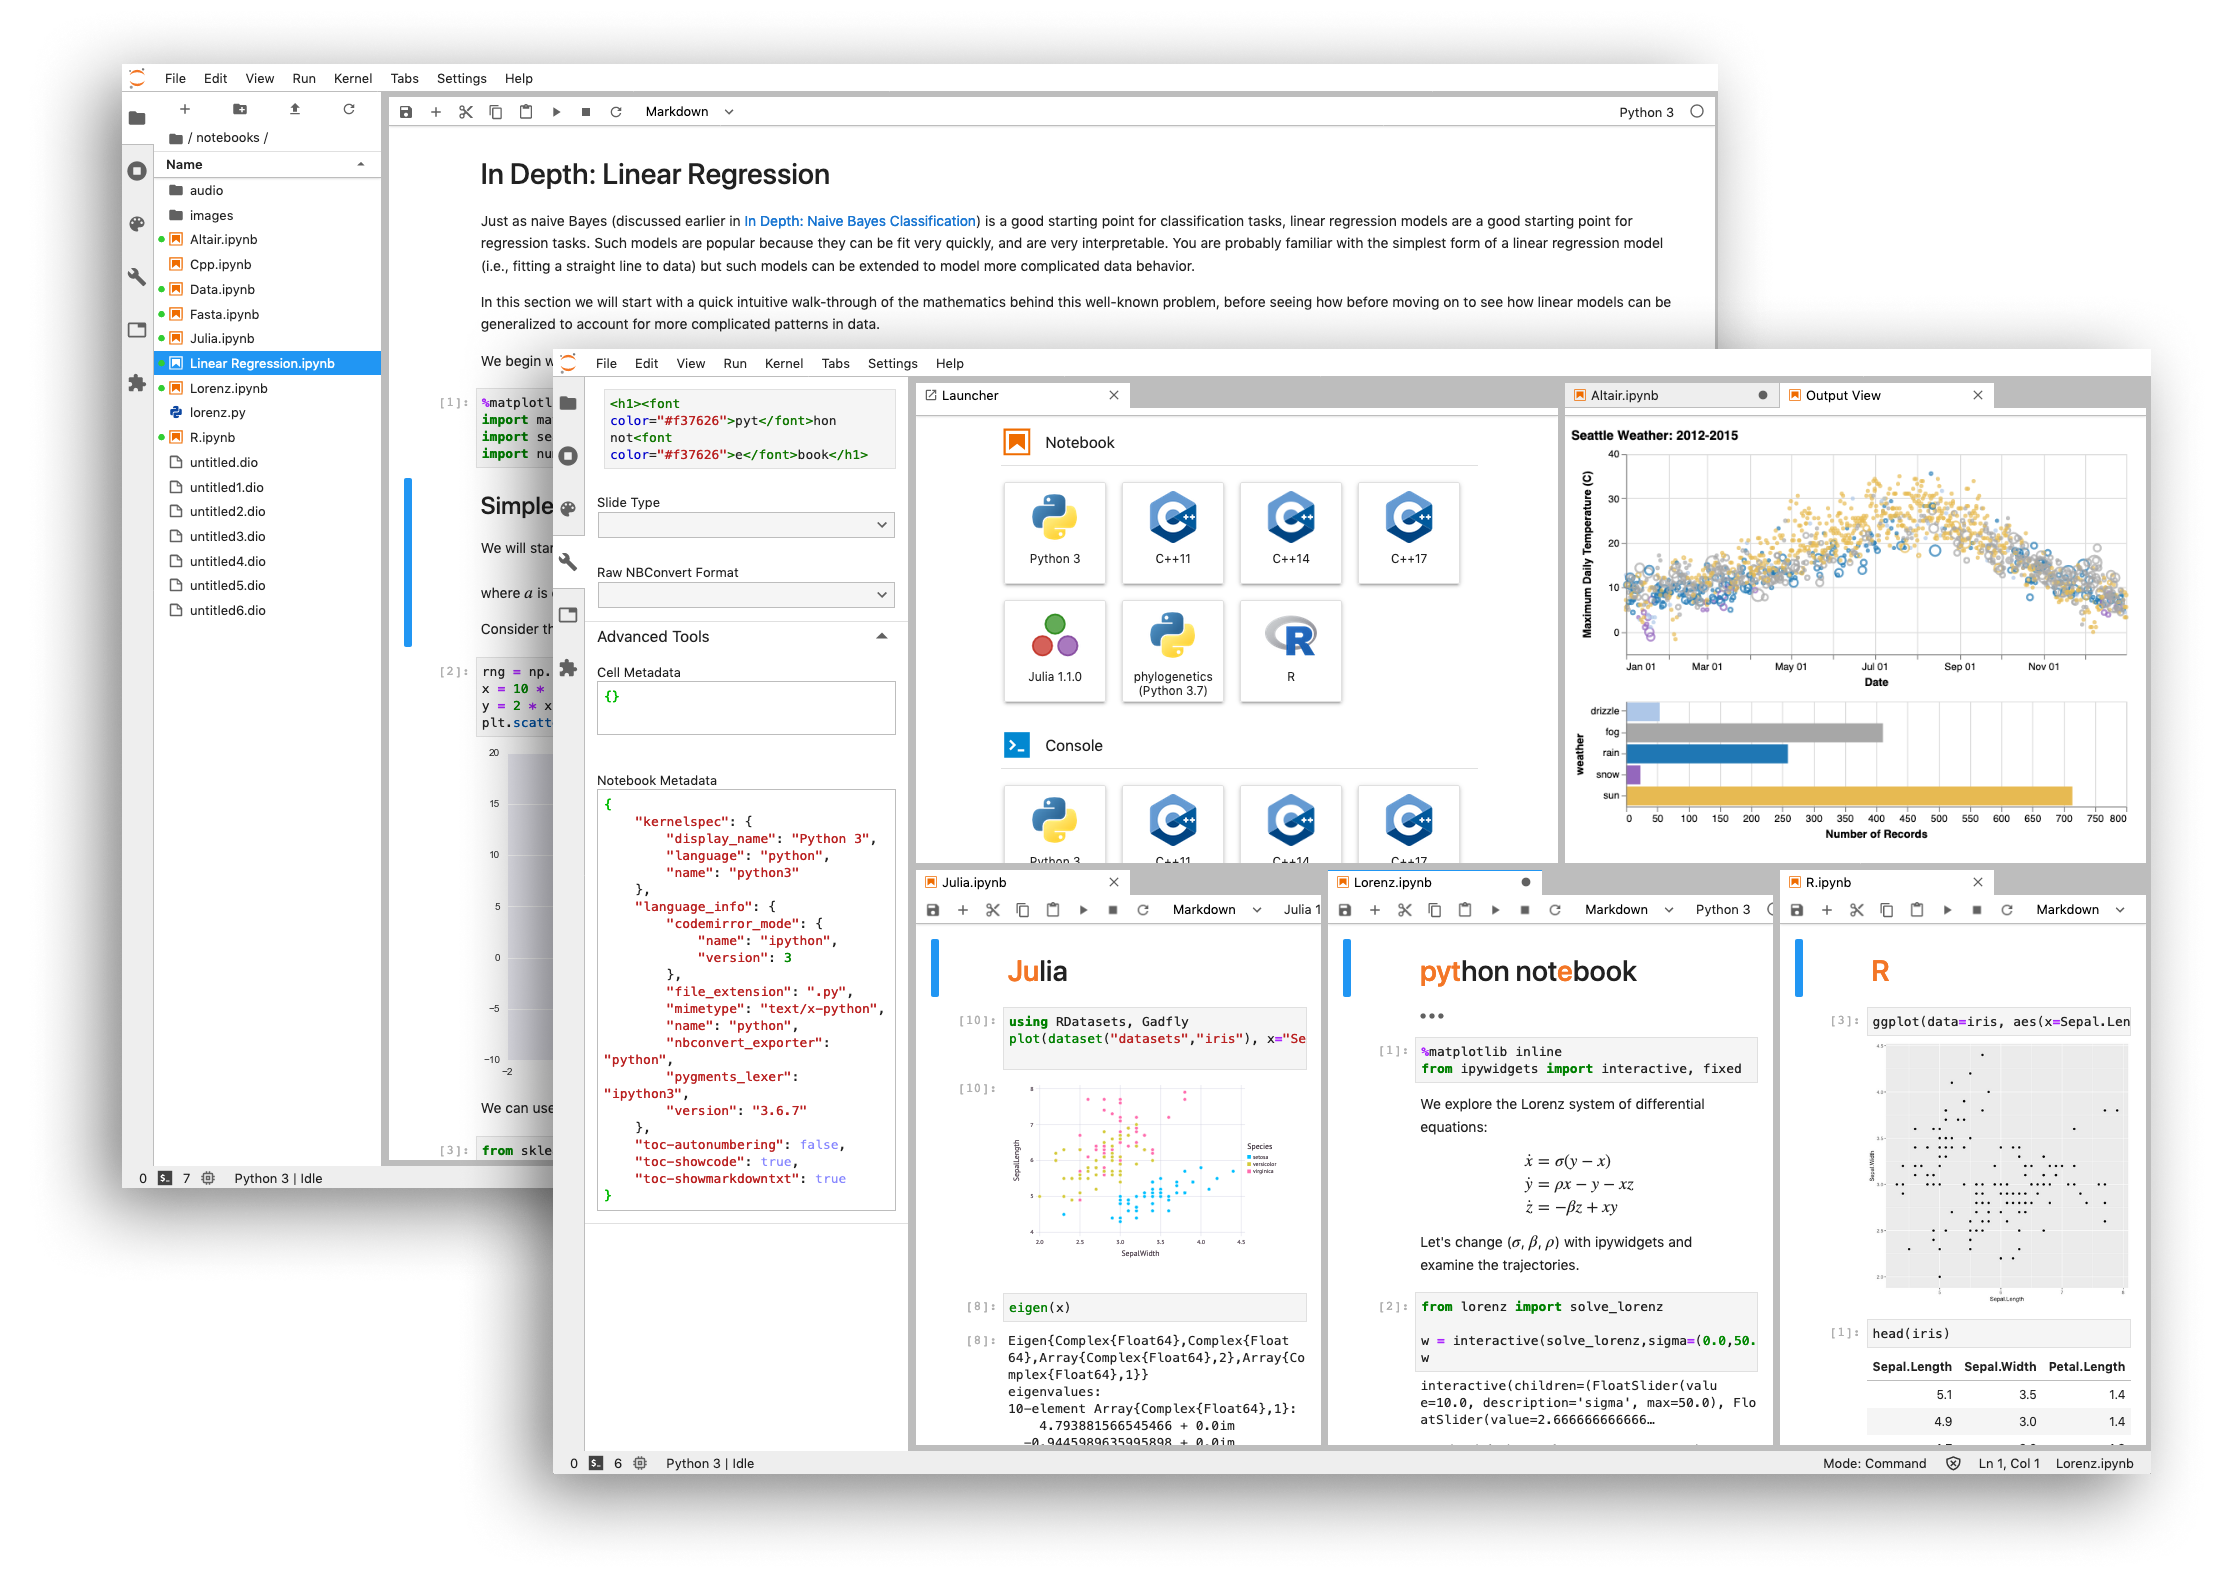
\includegraphics[width=1\textwidth,height=\textheight]{source/figures/jupyter.png}
\caption{Ejemplos de Jupyter Notebooks. Fuente: https://jupyter.org/
\label{jupyter}}
\end{figure}

En relación con el \textbf{hardware}, como todo proyecto de Deep
Learning, la tarjeta gráfica utilizada durante el entrenamiento ha
jugado un papel fundamental. En proyectos con grandes conjuntos de
imágenes, como es el caso, no disponer de tarjeta gráfica (o disponer de
una tarjeta sin la suficiente capacidad de procesamiento) puede hacer
inviable el entrenamiento de los modelos. En este caso, la tarjeta
gráfica utilizada ha sido la \textbf{NVIDIA TITAN Xp}. Esta tarjeta
cuenta con una \textbf{arquitectura Pascal} con una frecuencia de reloj
de 1481 MHz, y 12 GB de memoria. La potencia de cómputo de la NVIDIA
TITAN Xp es de 12.15 TFLOPS. Además, parte del procesamiento en local se
ha realizado en un \textbf{MacBook Air} con un procesador \textbf{Intel
Core i7 de 2.2 GHz} y 8 GB de memoria RAM.

\hypertarget{pre-procesado-de-las-imuxe1genes}{%
\section{Pre-procesado de las
imágenes}\label{pre-procesado-de-las-imuxe1genes}}

Las siguientes transformaciones han sido aplicadas a las imágenes
durante la fase de \textbf{pre-procesado}:

\begin{itemize}
\tightlist
\item
  \textbf{Reescalado del valor de los píxeles}: Dividiendo el valor de
  cada píxel entre 255 se obtienen únicamente valores entre 0 y 1, que
  son valores más comunes y, por lo tanto, más fáciles de manejar por
  los algoritmos de entrenamiento de las redes.
\item
  \textbf{Reescalado de las imágenes}: Todas las imágenes han sido
  reescaladas a un tamaño de 224x224. La elección de este tamaño se debe
  a que es el \textbf{tamaño de las imágenes del dataset Imagenet}.
  Puesto que los pesos que usaremos como punto de partida de nuestra red
  vienen de una red entrenada con este dataset, mantener un mismo tamaño
  de imagen permitirá poder reusar mejor algunos de los filtros
  aprendidos.
\end{itemize}

La técnica conocida como \textbf{Data Augmentation} ha sido utilizada en
todos los sistemas. Esta técnica permite añadir al conjunto de imágenes
de entrenamiento, nuevas imágenes que provienen de la aplicación de
diversas transformaciones a las imágenes del conjunto original. Esta
técnica supondrá, como es obvio, un aumento del número total de imágenes
del conjunto de entrenamiento y permitirá la obtención de clasificadores
capaces de generalizar mejor ante nuevos casos. Dependiendo de las
transformaciones utilizadas, el Data Augmentation permitirá la obtención
de clasificadores más robustos frente al ruido, traslación/rotación de
los objetos, a las variaciones del brillo, etc. En este caso, las
transformaciones utilizadas han sido:

\begin{itemize}
\tightlist
\item
  Inversión del eje horizontal
\item
  Aplicación de zoom aleatorio (hasta 1.25x)
\item
  Desplazamiento aleatorio en el eje horizontal (hasta 10\%)
\item
  Desplazamiento aleatorio en el eje vertical (hasta 10\%)
\item
  Modificación aleatoria del brillo (entre -50\% y +50\%)
\end{itemize}

La librería utilizada, \textbf{Keras}, ha simplificado en gran medida
este proceso. Las transformaciones elegidas y sus parámetros han sido
escogidas de tal forma que den lugar a imágenes \emph{coherentes} como
las que se podrían obtener con cualquier cámara de fondo de ojo.

\newpage

\hypertarget{diseuxf1o-del-sistema-1-gran-clasificador}{%
\section{Diseño del sistema 1: Gran
clasificador}\label{diseuxf1o-del-sistema-1-gran-clasificador}}

A continuación se presentarán las características de los sistemas de
clasificación realizados. Estos sistemas tienen como finalidad la
\textbf{detección de imágenes de retinas sanas, enfermas de RD o
enfermas de DMAE}. Sin embargo, en ningún momento ha sido objetivo de
este trabajo la detección de los diferentes niveles de gravedad de ambas
patologías, principalmente debido a la falta de suficientes conjuntos de
imágenes que proporcionen esta información para la fase de entrenamiento
de los modelos. Los 3 sistemas presentados a continuación son totalmente
independientes.

El primer sistema realizado (Figura \ref{des1}) se trata de una
\textbf{CNN basada en la arquitectura VGG16} (Simonyan \& Zisserman
2014) que trata de distinguir, de una sola vez, entre los 3 tipos de
imágenes (RD, DMAE, Sanas). A la salida de la última capa convolucional
se han añadido 3 capas de tipo \textbf{fully connected} con 2048, 1024 y
512 neuronas. Entre ellas, para evitar el \emph{overfitting} se han
intercalado capas de tipo \textbf{Dropout}. Por último, la capa de
salida cuenta con 3 neuronas (una por cada clase) y hace uso de la
función de activación \textbf{softmax}. Para entrenar esta red se han
utilizado las 39118 imágenes de todos los datasets descritos
anteriormente.

\begin{figure}
\centering
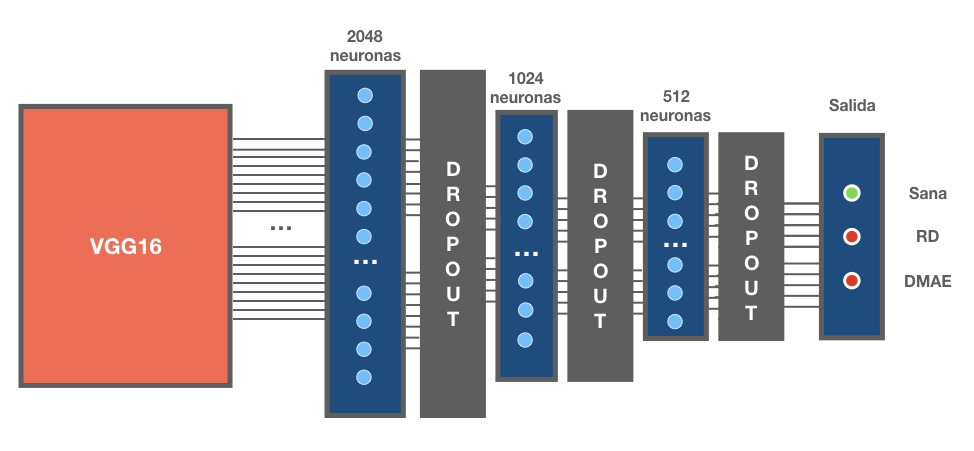
\includegraphics[width=1\textwidth,height=\textheight]{source/figures/design1_ar.png}
\caption{Arquitectura utilizada para el sistema 1. Elaboración propia
\label{des1}}
\end{figure}

El gran desbalanceo existente entre las clases, como se presentaba en la
tabla \ref{datasets1}, ha supuesto que este diseño no fuera capaz de
detectar correctamente las 3 clases que componen nuestro problema y, por
lo tanto, \textbf{ha sido desechado}.

\hypertarget{diseuxf1o-del-sistema-2-clasificador-multietapa}{%
\section{Diseño del sistema 2: Clasificador
Multietapa}\label{diseuxf1o-del-sistema-2-clasificador-multietapa}}

Los resultados del primer sistema ponen de manifiesto la necesidad de
aplicar técnicas que traten el problema del desbalanceo. Por ello, el
segundo sistema consta de \textbf{dos clasificadores binarios en
cascada} (Figura \ref{design2}):

\begin{itemize}
\item
  El primer clasificador diferencia entre \textbf{retinas sanas y
  retinas enfermas} (sin distinguir entre Retinopatía Diabética o
  Degeneración Macular).
\item
  El segundo clasificador diferencia, de entre las imágenes de retinas
  detectadas como enfermas en el paso anterior, si el paciente está
  afectado de \textbf{RD o de DMAE}.
\end{itemize}

\begin{figure}
\centering
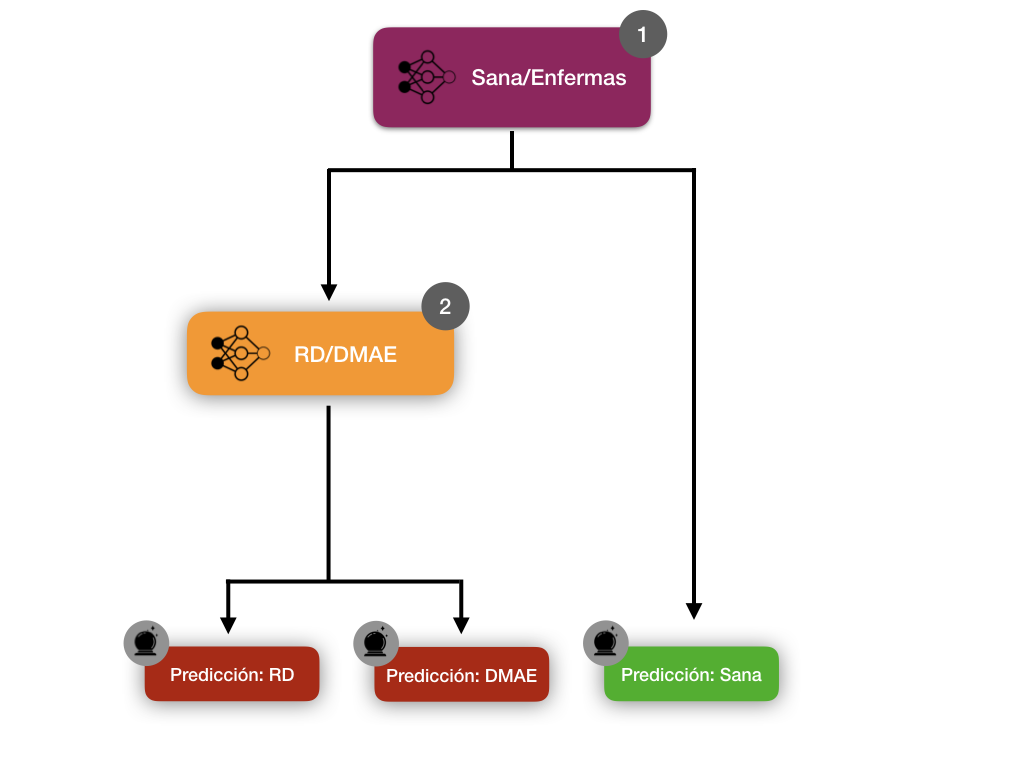
\includegraphics[width=1\textwidth,height=\textheight]{source/figures/design2.png}
\caption{Arquitectura del sistema clasificador en dos etapas Elaboración
propia \label{design2}}
\end{figure}

Gracias a este sistema basado en dos etapas se obtiene un desbalanceo
entre clases, en cada una de las etapas, inferior al del conjunto
original de imágenes. El primer clasificador \textbf{hace uso del
conjunto completo de imágenes} para el entrenamiento pero, como se ha
comentado, \textbf{únicamente es capaz de distinguir entre dos posibles
casos, retinas sanas y retinas enfermas}. En la tabla \ref{c1s2} vemos
la distribución de las imágenes de este primer clasificador en los
conjuntos de entrenamiento, validación y test.

\begin{longtable}[]{@{}lrrr@{}}
\caption{Distribución de las imágenes del clasificador Sano/Enfermo del
sistema 2. \label{c1s2}}\tabularnewline
\toprule
\begin{minipage}[b]{0.14\columnwidth}\raggedright
Conjunto\strut
\end{minipage} & \begin{minipage}[b]{0.20\columnwidth}\raggedleft
Clase\strut
\end{minipage} & \begin{minipage}[b]{0.18\columnwidth}\raggedleft
Total\strut
\end{minipage} & \begin{minipage}[b]{0.18\columnwidth}\raggedleft
Total (\%)\strut
\end{minipage}\tabularnewline
\midrule
\endfirsthead
\toprule
\begin{minipage}[b]{0.14\columnwidth}\raggedright
Conjunto\strut
\end{minipage} & \begin{minipage}[b]{0.20\columnwidth}\raggedleft
Clase\strut
\end{minipage} & \begin{minipage}[b]{0.18\columnwidth}\raggedleft
Total\strut
\end{minipage} & \begin{minipage}[b]{0.18\columnwidth}\raggedleft
Total (\%)\strut
\end{minipage}\tabularnewline
\midrule
\endhead
\begin{minipage}[t]{0.14\columnwidth}\raggedright
train\strut
\end{minipage} & \begin{minipage}[t]{0.20\columnwidth}\raggedleft
sana\strut
\end{minipage} & \begin{minipage}[t]{0.18\columnwidth}\raggedleft
17610\strut
\end{minipage} & \begin{minipage}[t]{0.18\columnwidth}\raggedleft
70.34\strut
\end{minipage}\tabularnewline
\begin{minipage}[t]{0.14\columnwidth}\raggedright
train\strut
\end{minipage} & \begin{minipage}[t]{0.20\columnwidth}\raggedleft
enferma\strut
\end{minipage} & \begin{minipage}[t]{0.18\columnwidth}\raggedleft
7425\strut
\end{minipage} & \begin{minipage}[t]{0.18\columnwidth}\raggedleft
29.66\strut
\end{minipage}\tabularnewline
\begin{minipage}[t]{0.14\columnwidth}\raggedright
valid\strut
\end{minipage} & \begin{minipage}[t]{0.20\columnwidth}\raggedleft
sana\strut
\end{minipage} & \begin{minipage}[t]{0.18\columnwidth}\raggedleft
4463\strut
\end{minipage} & \begin{minipage}[t]{0.18\columnwidth}\raggedleft
71.31\strut
\end{minipage}\tabularnewline
\begin{minipage}[t]{0.14\columnwidth}\raggedright
valid\strut
\end{minipage} & \begin{minipage}[t]{0.20\columnwidth}\raggedleft
enferma\strut
\end{minipage} & \begin{minipage}[t]{0.18\columnwidth}\raggedleft
1796\strut
\end{minipage} & \begin{minipage}[t]{0.18\columnwidth}\raggedleft
28.69\strut
\end{minipage}\tabularnewline
\begin{minipage}[t]{0.14\columnwidth}\raggedright
test\strut
\end{minipage} & \begin{minipage}[t]{0.20\columnwidth}\raggedleft
sana\strut
\end{minipage} & \begin{minipage}[t]{0.18\columnwidth}\raggedleft
5544\strut
\end{minipage} & \begin{minipage}[t]{0.18\columnwidth}\raggedleft
70.86\strut
\end{minipage}\tabularnewline
\begin{minipage}[t]{0.14\columnwidth}\raggedright
test\strut
\end{minipage} & \begin{minipage}[t]{0.20\columnwidth}\raggedleft
enferma\strut
\end{minipage} & \begin{minipage}[t]{0.18\columnwidth}\raggedleft
2280\strut
\end{minipage} & \begin{minipage}[t]{0.18\columnwidth}\raggedleft
29.14\strut
\end{minipage}\tabularnewline
\bottomrule
\end{longtable}

Para tratar el \textbf{desbalanceo} existente en esta \textbf{primera
etapa}, se ha hecho uso de una técnica basada en aplicar durante el
entrenamiento a las instancias de la clase minoritaria (en este caso, la
clase \textbf{enferma}) un peso que compense el desbalanceo en la
función de coste.

\newpage

Para la \textbf{segunda etapa} la aproximación ha sido distinta. Si se
hubiera usado el conjunto de imágenes completo, el desbalanceo hubiera
sido demasiado grande, imposible de abordar incluso por la técnica
utilizada anteriormente. En este caso, se ha hecho uso de la técnica
conocida como \textbf{subsampling o submuestreo}. Para evitar tener una
cantidad de imágenes de RD muy superior a la de DMAE se han
seleccionado, de forma aleatoria, un conjunto de imágenes de RD que
serán las utilizadas para el entrenamiento. De esta forma, se entrenará
el clasificador con la misma cantidad de imágenes de DR que de DMAE.

Esta arquitectura basada en dos etapas nos ha permitido usar la
totalidad de las imágenes para el entrenamiento sin necesidad de
entrenar modelos con datasets extremadamente desbalanceados (como era el
caso del sistema inicial).

En la Figura \ref{des2} podemos ver la arquitectura utilizada en los
clasificadores de ambos subsistemas. Como se puede comprobar, es
prácticamente igual a la del sistema 1, pero en este caso se elimina una
de las capas \textbf{fully connected}. El clasificador sano/enfermo
únicamente ha hecho uso de la arquitectura \textbf{VGG16}, mientras que
el clasificador RD/DMAE ha hecho uso de las 3 arquitecturas de la
imagen: \textbf{VGG16} (Simonyan \& Zisserman 2014), \textbf{Resnet50}
(He et~al. 2016) e \textbf{InceptionV3} (Szegedy et~al. 2016). Puesto
que ahora la salida de la red es binaria, se ha cambiado la función de
activación softmax utilizada anteriormente en la última capa por la
\textbf{función sigmoide}.

\begin{figure}
\centering
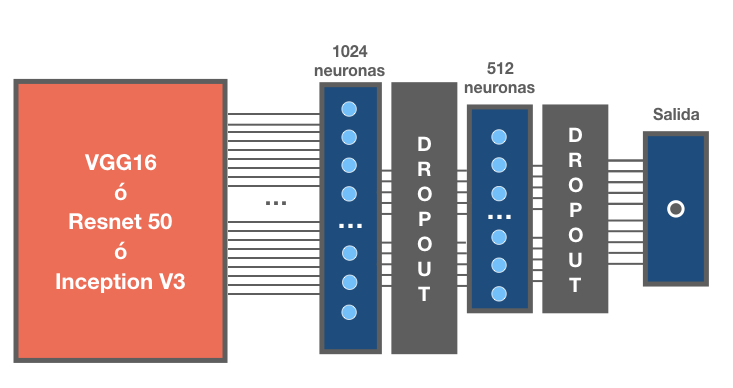
\includegraphics[width=1\textwidth,height=\textheight]{source/figures/des2.png}
\caption{Arquitectura utilizada para los clasificadores de ambos
subsistemas del segundo diseño. \label{des2}}
\end{figure}

Ambos clasificadores han utilizado la técnica del \textbf{Transfer
Learning}. Partiendo de los pesos originales procedentes de
\textbf{Imagenet}, se han realizado diversos entrenamientos, cambiando
el número de parámetros de la red \emph{congelados}:

\begin{itemize}
\tightlist
\item
  Entrenamiento únicamente de las capas fully-connected
\item
  Entrenamiento de las capas fully-connected y el bloque convolucional
  número 5: (Últimas 4 capas de la red convolucional)
\item
  Entrenamiento de las capas fully-connected y los bloques
  convolucionales 4 y 5: (Últimas 8 capas de la red convolucional)
\item
  Entrenamiento de las capas fully-connected y los bloques
  convolucionales 3, 4 y 5: (Últimas 12 capas de la red convolucional)
\item
  Entrenamiento de las capas fully-connected y los bloques
  convolucionales 2, 3, 4 y 5: (Últimas 15 capas de la red
  convolucional)
\item
  Entrenamiento de la red completa
\end{itemize}

Como se detallará en el siguiente capítulo, la ejecución de varios
entrenamientos alterando hiperparámetros como el \emph{learning rate} o
el \emph{batch size} ha permitido obtener los valores óptimos para
éstos.

\hypertarget{diseuxf1o-del-sistema-3-ensemble-de-clasificadores}{%
\section{Diseño del sistema 3: Ensemble de
Clasificadores}\label{diseuxf1o-del-sistema-3-ensemble-de-clasificadores}}

El tercer sistema diseñado permite detectar los 3 posibles casos (RD,
DMAE, y Sana) en una sola etapa a partir de la combinación de las
predicciones de 3 clasificadores entrenados con diferentes subconjuntos
de imágenes (Figura \ref{design3}). De esta forma, al igual que en el
caso anterior conseguimos entrenar modelos con la misma cantidad de
imágenes en cada clase.

\begin{figure}
\centering
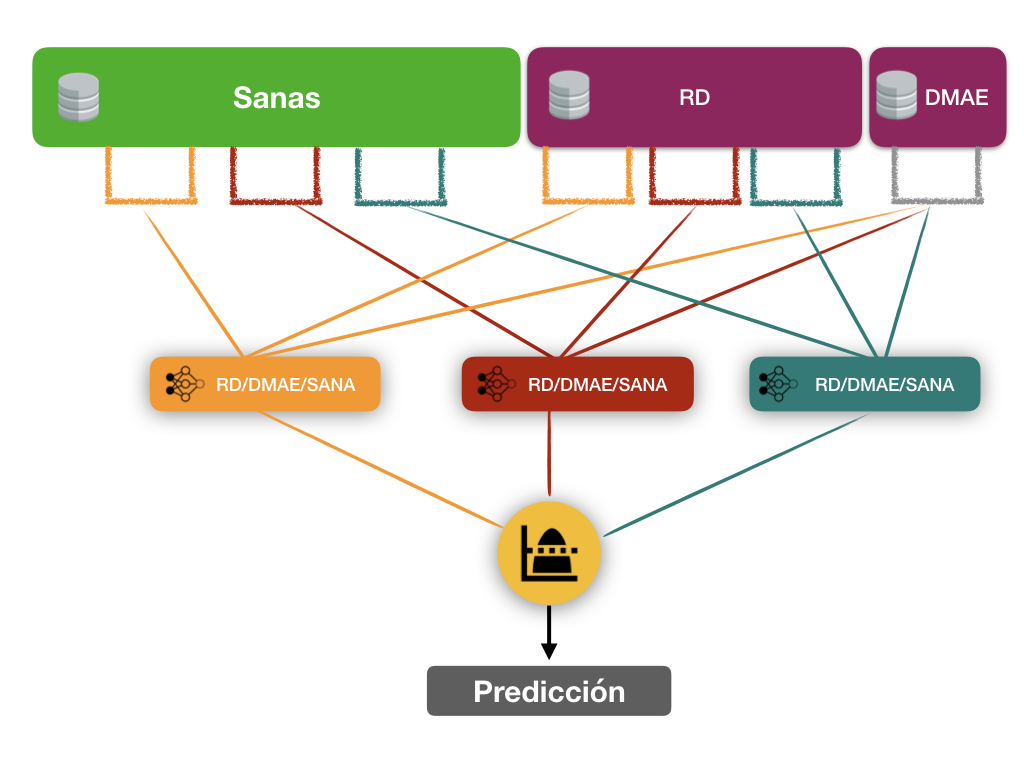
\includegraphics[width=1\textwidth,height=\textheight]{source/figures/design3.png}
\caption{Arquitectura del sistema de ensemble de clasificadores simples.
Los bloques superiores representan los conjuntos de imágenes utilizados
para el entrenamiento de los mismos Elaboración propia \label{design3}}
\end{figure}

De la misma forma que el sistema anterior, este sistema también ha
aplicado \textbf{Transfer Learning} descongelando progresivamente
bloques de capas hasta llegar a obtener la mejor evaluación posible con
el dataset de validación.

La arquitectura utilizada ha sido la misma que la de la Figura
\ref{des2} (aunque, en este caso, con 3 neuronas en la última capa, una
por cada posible clase de salida), entrenándose con las mismas 3
arquitecturas: VGG16, Resnet50 e InceptionV3.

\hypertarget{diseuxf1o-del-sistema-de-predicciuxf3n-e-interpretaciuxf3n}{%
\section{Diseño del Sistema de Predicción e
Interpretación}\label{diseuxf1o-del-sistema-de-predicciuxf3n-e-interpretaciuxf3n}}

Para hacer accesible el uso de los sistemas de predicción se ha diseñado
un pequeño software que abstrae la complejidad de todo el proceso,
permitiendo a los especialistas hacer uso de estos modelos simplemente
seleccionando las imágenes del paciente que se desea analizar. Para
ello, se ha hecho uso de las Jupyter Notebook explicadas anteriormente.

Mediante este programa, el usuario puede elegir el sistema que quiere
utilizar en cada caso: el Clasificador Multietapa, o el Ensemble de
Clasificadores. Una vez seleccionada la imagen de fondo de ojo a
analizar, el programa devolverá sus predicciones, el grado de confianza
y un mapa de calor procedente de la aplicación del algoritmmo
\textbf{Grad-Cam}.

En el capítulo \ref{resultados}, se analizan los resultados de diversas
ejecuciones del programa.

\hypertarget{resultados}{%
\chapter{Análisis de los resultados obtenidos}\label{resultados}}

Durante este capítulo se analiza el funcionamiento de los sistemas
descritos en el capítulo anterior. En todos los casos, el dataset
original ha sido dividido en 3 subgrupos, obteniendo así:

\begin{itemize}
\tightlist
\item
  \textbf{Dataset de entrenamiento}
\item
  \textbf{Dataset de validación}
\item
  \textbf{Dataset de test}
\end{itemize}

Los resultados que se presentan durante este capítulo son los
correspondientes a los datasets de validación y, en algunos casos, los
de test, puesto que la evaluación del clasificador con el conjunto de
datos de entrenamiento no es relevante para conocer la capacidad de
\textbf{generalización} de los sistemas. El dataset de validación ha
permitido evaluar el rendimiento de diferentes \textbf{arquitecturas e
hiperparámetros} mientras que el dataset de test ha permitido dar, al
final del proceso, una evaluación del sistema final con datos nuevos y
comprobar el funcionamiento del \textbf{Sistema de Predicción e
Interpretación}. Las métricas proporcionadas serán siempre las del
\textbf{mejor epoch}, es decir, el que ha obtenido el mínimo valor de
pérdidas con el dataset de validación.

Antes de pasar al análisis de los sistemas, es importante conocer cómo
se obtienen las métricas utilizadas, como se presenta durante la
siguiente sección.

\hypertarget{evaluaciuxf3n-de-sistemas-de-machine-learning}{%
\section{Evaluación de sistemas de Machine
Learning}\label{evaluaciuxf3n-de-sistemas-de-machine-learning}}

Un paso tan importante como el modelado en un proyecto de análisis de
datos es la evaluación de los resultados. Es de gran importancia
establecer medidas que nos permitan saber cómo se está comportando
nuestro modelo. En la literatura existe una gran cantidad de métricas,
aunque en este caso nos centraremos en algunas de las más comunes en
problemas de este tipo.

El problema analizado en este trabajo es un problema de
\textbf{clasificación}, es decir la variable objetivo (la que
predecimos) solo puede tomar un conjunto de valores discretos. Además,
lo que inicialmente era un problema con tres posibles clases
(RD/DMAE/Sano) también puede descomponerse en \textbf{dos problemas de
clasificación binaria} (RD/Sano) (DMAE/Sano). Se trata de predecir una
clase con sólo dos posibles valores. Cuando en un problema de este tipo
comparamos la predicción realizada por un modelo con el \emph{ground
truth} (es decir, la clase que realmente correspondería a esa
instancia), pueden darse 4 posibles casos:

\begin{itemize}
\tightlist
\item
  \textbf{Verdadero Positivo (o True Positive, TP)}: El sistema predice
  que el paciente \textbf{SÍ} tiene la enfermedad y acierta.
\item
  \textbf{Verdadero Negativo (o True Negative, TN)}: El sistema predice
  que el paciente \textbf{NO} tiene la enfermedad y acierta.
\item
  \textbf{Falso Negativo (o False Negative, FN)}: El sistema predice,
  erróneamente, que el paciente \textbf{NO} tiene la enfermedad cuando
  en realidad sí que la tiene.
\item
  \textbf{Falso Positivo (o False Positive, FP)}: El sistema predice,
  erróneamente, que el paciente \textbf{SÍ} tiene la enfermedad cuando
  en realidad no la tiene.
\end{itemize}

A partir de la cantidad de predicciones de cada uno de estos posibles 4
tipos se pueden definir una serie de medidas muy comunes en problemas de
este tipo.

La métrica más común, conocida como \textbf{Accuracy} o
\textbf{Exactitud}, mide el porcentaje de aciertos del sistema (ecuacion
\ref{eq:accuracy}). Esta métrica carece de utilidad cuando tenemos
conjuntos de datos desbalanceados.

\begin{equation} \label{eq:accuracy}
 \frac{TP+TN}{TP+TN+FN+FP}
\end{equation}

La \textbf{Sensibilidad} mide la proporción de los pacientes que
\textbf{Sí} tienen la enfermedad que nuestro clasificador ha sido capaz
de detectar (ecuación \ref{eq:sensibilidad})

\begin{equation} \label{eq:sensibilidad}
 \frac{TP}{TP+FN}
\end{equation}

La \textbf{Especificidad}, en cambio, mide proporción de los pacientes
que \textbf{No} tienen la enfermedad que nuestro clasificador ha sido
capaz de detectar (ecuacion \ref{eq:especificidad})

\begin{equation} \label{eq:especificidad}
 \frac{TN}{TN+FP}
\end{equation}

En función del campo de aplicación de los modelos, unas métricas toman
más importancia que otras. Incluso es común tener \textbf{umbrales de
actuación} en nuestros modelos que nos permitan elegir el punto de
equilibrio deseado entre sensibilidad y especificidad. Un modelo que
trata de predecir la presencia de una enfermedad siempre tratará de
enfocarse más en obtener una buena \textbf{sensibilidad} antes de
centrarse en la \textbf{especificidad}. El coste de predecir
erróneamente que un paciente tiene una enfermedad, es menor al de no
haber detectado la enfermedad en un paciente que sí que la tenía.

\hypertarget{evaluaciuxf3n-del-sistema-1-gran-clasificador}{%
\section{Evaluación del Sistema 1: Gran
Clasificador}\label{evaluaciuxf3n-del-sistema-1-gran-clasificador}}

Como ya se anunciaba en el capítulo \ref{sistema}, debido al gran
desbalanceo existente entre las clases, este sistema \textbf{no nos ha
permitido distinguir correctamente entre las 3 clases}. Tras evaluarse
varios valores distintos para el \emph{learning rate} y \emph{batch
size} e incluso añadirse pesos a las clases que compensaran el
desbalanceo existente, el proceso de descenso de gradiente ha quedado
constantemente \emph{atrapado} en mínimos locales en los que el
clasificador predice la misma clase para todas las instancias.
Concluimos, por lo tanto, que \textbf{un solo clasificador no tiene
capacidad suficiente para obtener patrones de un conjunto de datos tan
desbalanceado} y habrá que buscar soluciones alternativas.

\hypertarget{evaluaciuxf3n-del-sistema-2-clasificador-multietapa}{%
\section{Evaluación del Sistema 2: Clasificador
Multietapa}\label{evaluaciuxf3n-del-sistema-2-clasificador-multietapa}}

El segundo sistema consta de 2 etapas: la clasificación
\textbf{Sano/Enfermo} y la clasificación \textbf{RD/DMAE}. Ambas etapas
son analizadas a continuación.

\hypertarget{etapa-1-clasificador-sanoenfermo}{%
\subsection{Etapa 1: Clasificador
Sano/Enfermo}\label{etapa-1-clasificador-sanoenfermo}}

Las 39118 imágenes de las que se componía nuestro cojunto de imágenes
inicial han sido divididas en 2 grupos: \textbf{Retinas Sanas y Retinas
Enfermas}.

Puesto que ha sido utilizada la técnica de \textbf{Transfer Learning},
se han realizado varias ejecuciones descongelando, progresivamente cada
uno de los bloques convolucionales de la arquitectura utilizada,
\textbf{VGG16}. Esta arquitectura posee 5 bloques convolucionales con
\textbf{capas de pooling} en cada uno de estos bloques.

Inicialmente se han realizado varios entrenamientos del bloque
\emph{fully connected} para evaluar los posibles \emph{batch size} y
\emph{learning rate}. La tabla \ref{batch} contiene los resultados
obtenidos para distintos \emph{batch sizes}. Las evaluaciones de la
tabla son las correspondientes al dataset de validación para el mejor
epoch.\footnote{el que tiene menores pérdidas con el dataset de
  validación} El \emph{learning rate} utilizado ha sido de 0.0001.

\newpage

\begin{longtable}[]{@{}rcc@{}}
\caption{Resultados del entrenamiento para distintos batch size. Modelos
evaluados con el dataset de validación \label{batch}}\tabularnewline
\toprule
\begin{minipage}[b]{0.16\columnwidth}\raggedleft
batch size\strut
\end{minipage} & \begin{minipage}[b]{0.15\columnwidth}\centering
accuracy\strut
\end{minipage} & \begin{minipage}[b]{0.15\columnwidth}\centering
loss\strut
\end{minipage}\tabularnewline
\midrule
\endfirsthead
\toprule
\begin{minipage}[b]{0.16\columnwidth}\raggedleft
batch size\strut
\end{minipage} & \begin{minipage}[b]{0.15\columnwidth}\centering
accuracy\strut
\end{minipage} & \begin{minipage}[b]{0.15\columnwidth}\centering
loss\strut
\end{minipage}\tabularnewline
\midrule
\endhead
\begin{minipage}[t]{0.16\columnwidth}\raggedleft
16\strut
\end{minipage} & \begin{minipage}[t]{0.15\columnwidth}\centering
0.7062\strut
\end{minipage} & \begin{minipage}[t]{0.15\columnwidth}\centering
0.5973\strut
\end{minipage}\tabularnewline
\begin{minipage}[t]{0.16\columnwidth}\raggedleft
32\strut
\end{minipage} & \begin{minipage}[t]{0.15\columnwidth}\centering
0.6782\strut
\end{minipage} & \begin{minipage}[t]{0.15\columnwidth}\centering
0.6151\strut
\end{minipage}\tabularnewline
\begin{minipage}[t]{0.16\columnwidth}\raggedleft
64\strut
\end{minipage} & \begin{minipage}[t]{0.15\columnwidth}\centering
0.7072\strut
\end{minipage} & \begin{minipage}[t]{0.15\columnwidth}\centering
0.6073\strut
\end{minipage}\tabularnewline
\bottomrule
\end{longtable}

A partir de la tabla \ref{batch} se puede intuir que el tamaño del
\emph{batch size} no juega un papel de gran importancia en el proceso de
entrenamiento por lo que se ha decidido usar, a partir de este momento
un tamaño de \textbf{64}. Este tamaño nos permite entrenar la red de
forma más rápida y nos asegura que en cada \emph{batch} exista
suficiente cantidad de imágenes de las dos clases. Usar tamaños
superiores habría ocasionado problemas de memoria en la GPU utilizada.

De la misma forma, como se aprecia en la tabla \ref{lr}, también se han
realizado varios entrenamientos del clasificador que nos han permitido
comprobar cuál es el \emph{learning rate} adecuado para nuestro
problema. Para ello se ha utilizado un \emph{batch size de 64}.

\begin{longtable}[]{@{}ccc@{}}
\caption{Resultados del entrenamiento para distintos learning rate.
Modelos evaluados con el dataset de validación
\label{lr}}\tabularnewline
\toprule
\begin{minipage}[b]{0.22\columnwidth}\centering
learning rate\strut
\end{minipage} & \begin{minipage}[b]{0.16\columnwidth}\centering
accuracy\strut
\end{minipage} & \begin{minipage}[b]{0.13\columnwidth}\centering
loss\strut
\end{minipage}\tabularnewline
\midrule
\endfirsthead
\toprule
\begin{minipage}[b]{0.22\columnwidth}\centering
learning rate\strut
\end{minipage} & \begin{minipage}[b]{0.16\columnwidth}\centering
accuracy\strut
\end{minipage} & \begin{minipage}[b]{0.13\columnwidth}\centering
loss\strut
\end{minipage}\tabularnewline
\midrule
\endhead
\begin{minipage}[t]{0.22\columnwidth}\centering
0.001\strut
\end{minipage} & \begin{minipage}[t]{0.16\columnwidth}\centering
0.287\strut
\end{minipage} & \begin{minipage}[t]{0.13\columnwidth}\centering
11.4\strut
\end{minipage}\tabularnewline
\begin{minipage}[t]{0.22\columnwidth}\centering
0.0001\strut
\end{minipage} & \begin{minipage}[t]{0.16\columnwidth}\centering
0.6782\strut
\end{minipage} & \begin{minipage}[t]{0.13\columnwidth}\centering
0.6151\strut
\end{minipage}\tabularnewline
\begin{minipage}[t]{0.22\columnwidth}\centering
0.00005\strut
\end{minipage} & \begin{minipage}[t]{0.16\columnwidth}\centering
0.7199\strut
\end{minipage} & \begin{minipage}[t]{0.13\columnwidth}\centering
0.6037\strut
\end{minipage}\tabularnewline
\bottomrule
\end{longtable}

Como se ha podido comprobar, utilizar un \emph{learning rate} demasiado
alto provoca que el descenso de gradiente quede \emph{atrapado} en
mínimos locales o no sea capaz de converger, dando lugar a unos valores
de pérdidas demasiado altos. El \textbf{learning rate de 0.0005} es el
que nos da mejores resultados y por lo tanto ha sido utilizado en los
posteriores entrenamientos. Este valor tendrá que disminuirse
ligeramente cuando entrenemos varias capas convolucionales a la vez para
asegurarnos un descenso de gradiente lento que pueda converger en un
mínimo absoluto.

Una vez decididos los hiperparámetros se ha comenzado a
\emph{descongelar} los diversos bloques de las capas convolucionales de
la red, obteniendo los resultados de la tabla \ref{training}

\begin{longtable}[]{@{}lclcll@{}}
\caption{Resultados del entrenamiento para distintos bloques
convolucionales entrenados. Modelos evaluados con el dataset de
validación \label{training}}\tabularnewline
\toprule
\begin{minipage}[b]{0.20\columnwidth}\raggedright
train blocks\strut
\end{minipage} & \begin{minipage}[b]{0.10\columnwidth}\centering
LR\strut
\end{minipage} & \begin{minipage}[b]{0.14\columnwidth}\raggedright
accuracy\strut
\end{minipage} & \begin{minipage}[b]{0.11\columnwidth}\centering
loss\strut
\end{minipage} & \begin{minipage}[b]{0.17\columnwidth}\raggedright
sensitivity\strut
\end{minipage} & \begin{minipage}[b]{0.11\columnwidth}\raggedright
specifity\strut
\end{minipage}\tabularnewline
\midrule
\endfirsthead
\toprule
\begin{minipage}[b]{0.20\columnwidth}\raggedright
train blocks\strut
\end{minipage} & \begin{minipage}[b]{0.10\columnwidth}\centering
LR\strut
\end{minipage} & \begin{minipage}[b]{0.14\columnwidth}\raggedright
accuracy\strut
\end{minipage} & \begin{minipage}[b]{0.11\columnwidth}\centering
loss\strut
\end{minipage} & \begin{minipage}[b]{0.17\columnwidth}\raggedright
sensitivity\strut
\end{minipage} & \begin{minipage}[b]{0.11\columnwidth}\raggedright
specifity\strut
\end{minipage}\tabularnewline
\midrule
\endhead
\begin{minipage}[t]{0.20\columnwidth}\raggedright
FC\strut
\end{minipage} & \begin{minipage}[t]{0.10\columnwidth}\centering
5e-5\strut
\end{minipage} & \begin{minipage}[t]{0.14\columnwidth}\raggedright
0.7149\strut
\end{minipage} & \begin{minipage}[t]{0.11\columnwidth}\centering
0.6549\strut
\end{minipage} & \begin{minipage}[t]{0.17\columnwidth}\raggedright
0.1713\strut
\end{minipage} & \begin{minipage}[t]{0.11\columnwidth}\raggedright
0.9338\strut
\end{minipage}\tabularnewline
\begin{minipage}[t]{0.20\columnwidth}\raggedright
Bloque 5\strut
\end{minipage} & \begin{minipage}[t]{0.10\columnwidth}\centering
5e-5\strut
\end{minipage} & \begin{minipage}[t]{0.14\columnwidth}\raggedright
0.7532\strut
\end{minipage} & \begin{minipage}[t]{0.11\columnwidth}\centering
0.5294\strut
\end{minipage} & \begin{minipage}[t]{0.17\columnwidth}\raggedright
0.3805\strut
\end{minipage} & \begin{minipage}[t]{0.11\columnwidth}\raggedright
0.9012\strut
\end{minipage}\tabularnewline
\begin{minipage}[t]{0.20\columnwidth}\raggedright
Bloques 4,5\strut
\end{minipage} & \begin{minipage}[t]{0.10\columnwidth}\centering
5e-6\strut
\end{minipage} & \begin{minipage}[t]{0.14\columnwidth}\raggedright
0.7126\strut
\end{minipage} & \begin{minipage}[t]{0.11\columnwidth}\centering
0.6854\strut
\end{minipage} & \begin{minipage}[t]{0.17\columnwidth}\raggedright
0\strut
\end{minipage} & \begin{minipage}[t]{0.11\columnwidth}\raggedright
1\strut
\end{minipage}\tabularnewline
\begin{minipage}[t]{0.20\columnwidth}\raggedright
Bloques 3,4,5\strut
\end{minipage} & \begin{minipage}[t]{0.10\columnwidth}\centering
5e-6\strut
\end{minipage} & \begin{minipage}[t]{0.14\columnwidth}\raggedright
0.7880\strut
\end{minipage} & \begin{minipage}[t]{0.11\columnwidth}\centering
0.4748\strut
\end{minipage} & \begin{minipage}[t]{0.17\columnwidth}\raggedright
0.4793\strut
\end{minipage} & \begin{minipage}[t]{0.11\columnwidth}\raggedright
0.9131\strut
\end{minipage}\tabularnewline
\begin{minipage}[t]{0.20\columnwidth}\raggedright
Bloques 2,3,4,5\strut
\end{minipage} & \begin{minipage}[t]{0.10\columnwidth}\centering
5e-6\strut
\end{minipage} & \begin{minipage}[t]{0.14\columnwidth}\raggedright
0.7961\strut
\end{minipage} & \begin{minipage}[t]{0.11\columnwidth}\centering
0.4704\strut
\end{minipage} & \begin{minipage}[t]{0.17\columnwidth}\raggedright
0.5867\strut
\end{minipage} & \begin{minipage}[t]{0.11\columnwidth}\raggedright
0.8624\strut
\end{minipage}\tabularnewline
\begin{minipage}[t]{0.20\columnwidth}\raggedright
Todos\strut
\end{minipage} & \begin{minipage}[t]{0.10\columnwidth}\centering
5e-6\strut
\end{minipage} & \begin{minipage}[t]{0.14\columnwidth}\raggedright
0.8015\strut
\end{minipage} & \begin{minipage}[t]{0.11\columnwidth}\centering
0.4604\strut
\end{minipage} & \begin{minipage}[t]{0.17\columnwidth}\raggedright
0.4680\strut
\end{minipage} & \begin{minipage}[t]{0.11\columnwidth}\raggedright
0.9364\strut
\end{minipage}\tabularnewline
\bottomrule
\end{longtable}

Como se puede ver en la tabla \ref{training}, \textbf{los mejores
resultados se han obtenido al entrenar todos los bloques
convolucionales}, obteniendo una \emph{accuracy} de 80.15\%. Sin
embargo, será la versión de la red en la que se han entrenado los
bloques 2, 3, 4 y 5 la que se usará en el \textbf{Sistema de Predicción
e Interpretación} para la segunda etapa del Clasificador Multietapa.
Esta versión tiene una sensibilidad notablemente superior, con unas
pérdidas similares a las de la red que ofrece las mínimas pérdidas. Cabe
destacar que, a partir del entrenamiento del bloque 4, hemos tenido que
disminuir el \emph{learning rate} para evitar caer en mínimos locales y
asegurar la convergencia.

Debido a la gran carga computacional que ha supuesto entrenar este
modelo (cada entrenamiento ha durado una media de 72 horas), únicamente
se ha evaluado la arquitectura \textbf{VGG16}.

\begin{figure}
\centering
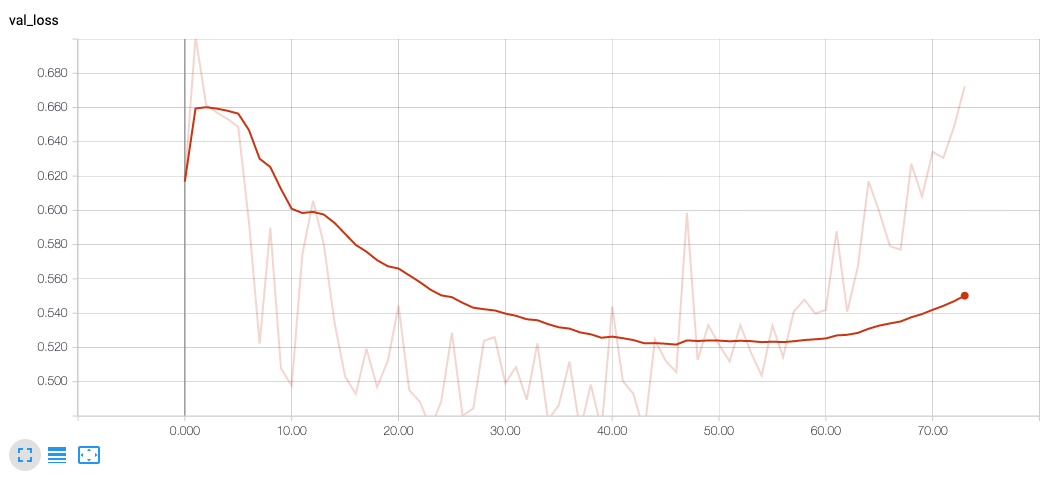
\includegraphics[width=1\textwidth,height=\textheight]{source/figures/loss1.png}
\caption{Pérdidas para el dataset de validación del entrenamiento de los
bloques 2,3,4 y 5 (y FC) del clasificador Sano/Enfermo. Se ha aplicado
un filtro de suavizado. \label{valloss}}
\end{figure}

La Figura \ref{valloss} contiene la progresión de las pérdidas durante
el entrenamiento del clasificador final elegido para esta etapa.
\textbf{Las mínimas pérdidas se obtienen alrededor del epoch 45}. A
partir de ese momento, la red empieza a sufrir de \emph{overfitting} y
las pérdidas con el dataset de validación aumentarán mientras que las
del dataset de entrenamiento continuarán descendiendo. Esto es un claro
indicador de que la red está comenzando a \textbf{memorizar} el dataset
de entrenamiento en vez de detectar y aprender patrones. Por lo tanto,
nos quedaremos con el estado de la red en ese epoch 45.

\begin{figure}
\centering
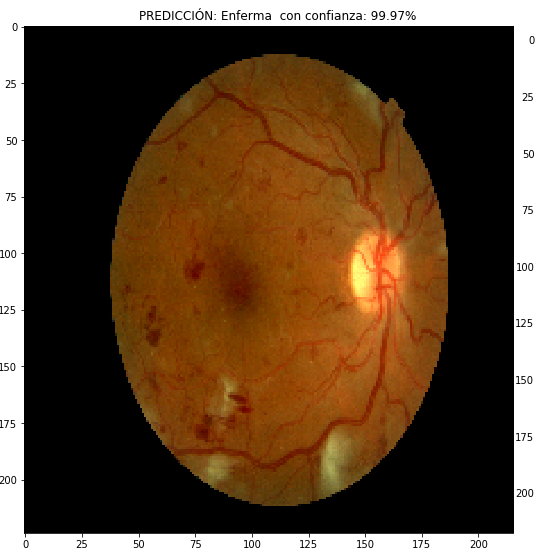
\includegraphics[width=0.7\textwidth,height=\textheight]{source/figures/hnh1.png}
\caption{Salida de la primera etapa del Sistema Multietapa para una
imagen de una retina enferma de RD \label{hnh1}}
\end{figure}

\begin{figure}
\centering
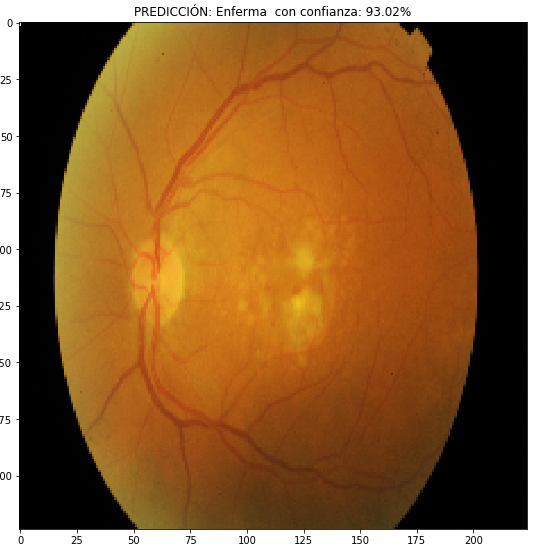
\includegraphics[width=0.7\textwidth,height=\textheight]{source/figures/hnh2.png}
\caption{Salida de la primera etapa del Sistema Multietapa para una
imagen de una retina enferma de DMAE \label{hnh2}}
\end{figure}

\begin{figure}
\centering
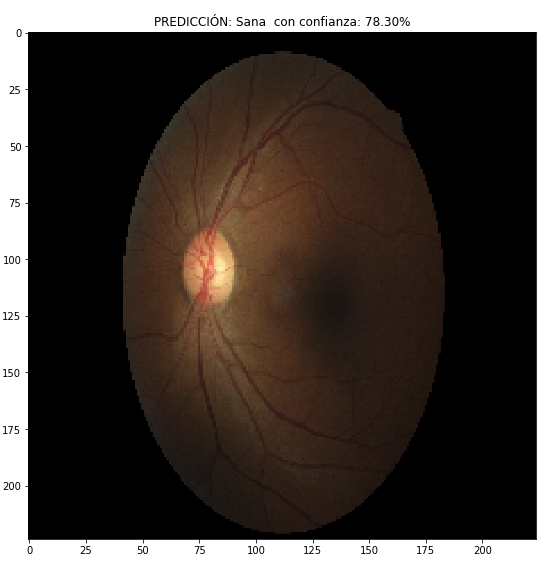
\includegraphics[width=0.7\textwidth,height=\textheight]{source/figures/hnh3.png}
\caption{Salida de la primera etapa del Sistema Multietapa para una
imagen de una retina sana \label{hnh3}}
\end{figure}

En las Figuras \ref{hnh1}, \ref{hnh2} y \ref{hnh3} se pueden ver
ejemplos de la respuesta proporcionada por esta etapa del sistema.

\newpage

\hypertarget{etapa-2-clasificador-rddmae}{%
\subsection{Etapa 2: Clasificador
RD/DMAE}\label{etapa-2-clasificador-rddmae}}

La tabla \ref{training2} muestra los resultados del entrenamiento de la
arquitectura \textbf{VGG16} para la \textbf{segunda etapa} del
\textbf{Sistema Multietapa}. La función de este clasificador es
diferenciar, de entre las imágenes de retinas detectadas como enfermas
en la etapa 1, cuáles sufren Retinopatía Diabética y cuáles Degeneración
Macular Asociada a la Edad.

\begin{longtable}[]{@{}lclc@{}}
\caption{Resultados del entrenamiento de la segunda etapa del Sistema
Multietapa. Modelos evaluados con el dataset de validación
\label{training2}}\tabularnewline
\toprule
\begin{minipage}[b]{0.22\columnwidth}\raggedright
train blocks\strut
\end{minipage} & \begin{minipage}[b]{0.11\columnwidth}\centering
LR\strut
\end{minipage} & \begin{minipage}[b]{0.15\columnwidth}\raggedright
accuracy\strut
\end{minipage} & \begin{minipage}[b]{0.11\columnwidth}\centering
loss\strut
\end{minipage}\tabularnewline
\midrule
\endfirsthead
\toprule
\begin{minipage}[b]{0.22\columnwidth}\raggedright
train blocks\strut
\end{minipage} & \begin{minipage}[b]{0.11\columnwidth}\centering
LR\strut
\end{minipage} & \begin{minipage}[b]{0.15\columnwidth}\raggedright
accuracy\strut
\end{minipage} & \begin{minipage}[b]{0.11\columnwidth}\centering
loss\strut
\end{minipage}\tabularnewline
\midrule
\endhead
\begin{minipage}[t]{0.22\columnwidth}\raggedright
FC\strut
\end{minipage} & \begin{minipage}[t]{0.11\columnwidth}\centering
1e-5\strut
\end{minipage} & \begin{minipage}[t]{0.15\columnwidth}\raggedright
0.9231\strut
\end{minipage} & \begin{minipage}[t]{0.11\columnwidth}\centering
0.1910\strut
\end{minipage}\tabularnewline
\begin{minipage}[t]{0.22\columnwidth}\raggedright
Bloque 5\strut
\end{minipage} & \begin{minipage}[t]{0.11\columnwidth}\centering
1e-5\strut
\end{minipage} & \begin{minipage}[t]{0.15\columnwidth}\raggedright
0.9359\strut
\end{minipage} & \begin{minipage}[t]{0.11\columnwidth}\centering
0.1483\strut
\end{minipage}\tabularnewline
\begin{minipage}[t]{0.22\columnwidth}\raggedright
Bloques 4,5\strut
\end{minipage} & \begin{minipage}[t]{0.11\columnwidth}\centering
1e-5\strut
\end{minipage} & \begin{minipage}[t]{0.15\columnwidth}\raggedright
0.8958\strut
\end{minipage} & \begin{minipage}[t]{0.11\columnwidth}\centering
0.2093\strut
\end{minipage}\tabularnewline
\begin{minipage}[t]{0.22\columnwidth}\raggedright
Bloques 3,4,5\strut
\end{minipage} & \begin{minipage}[t]{0.11\columnwidth}\centering
1e-5\strut
\end{minipage} & \begin{minipage}[t]{0.15\columnwidth}\raggedright
0.9615\strut
\end{minipage} & \begin{minipage}[t]{0.11\columnwidth}\centering
0.1443\strut
\end{minipage}\tabularnewline
\begin{minipage}[t]{0.22\columnwidth}\raggedright
Bloques 2,3,4,5\strut
\end{minipage} & \begin{minipage}[t]{0.11\columnwidth}\centering
1e-5\strut
\end{minipage} & \begin{minipage}[t]{0.15\columnwidth}\raggedright
0.9103\strut
\end{minipage} & \begin{minipage}[t]{0.11\columnwidth}\centering
0.1773\strut
\end{minipage}\tabularnewline
\begin{minipage}[t]{0.22\columnwidth}\raggedright
Todos\strut
\end{minipage} & \begin{minipage}[t]{0.11\columnwidth}\centering
1e-5\strut
\end{minipage} & \begin{minipage}[t]{0.15\columnwidth}\raggedright
0.9487\strut
\end{minipage} & \begin{minipage}[t]{0.11\columnwidth}\centering
0.1691\strut
\end{minipage}\tabularnewline
\bottomrule
\end{longtable}

Además, como muestra la tabla \ref{training3}, también se han entrenado
otras arquitecturas. En este caso, en vez de realizarse
\emph{fine-tuning}, se han entrenado todos los bloques convolucionales
de las mismas.

\begin{longtable}[]{@{}lclc@{}}
\caption{Resultados del entrenamiento de la segunda etapa del Sistema
Multietapa. Modelos evaluados con el dataset de validación
\label{training3}}\tabularnewline
\toprule
\begin{minipage}[b]{0.22\columnwidth}\raggedright
Arquitectura\strut
\end{minipage} & \begin{minipage}[b]{0.11\columnwidth}\centering
LR\strut
\end{minipage} & \begin{minipage}[b]{0.15\columnwidth}\raggedright
accuracy\strut
\end{minipage} & \begin{minipage}[b]{0.11\columnwidth}\centering
loss\strut
\end{minipage}\tabularnewline
\midrule
\endfirsthead
\toprule
\begin{minipage}[b]{0.22\columnwidth}\raggedright
Arquitectura\strut
\end{minipage} & \begin{minipage}[b]{0.11\columnwidth}\centering
LR\strut
\end{minipage} & \begin{minipage}[b]{0.15\columnwidth}\raggedright
accuracy\strut
\end{minipage} & \begin{minipage}[b]{0.11\columnwidth}\centering
loss\strut
\end{minipage}\tabularnewline
\midrule
\endhead
\begin{minipage}[t]{0.22\columnwidth}\raggedright
InceptionV3 Resnet50\strut
\end{minipage} & \begin{minipage}[t]{0.11\columnwidth}\centering
1e-5 1e-5\strut
\end{minipage} & \begin{minipage}[t]{0.15\columnwidth}\raggedright
0.9167 0.9744\strut
\end{minipage} & \begin{minipage}[t]{0.11\columnwidth}\centering
0.263 0.0816\strut
\end{minipage}\tabularnewline
\bottomrule
\end{longtable}

\begin{figure}
\centering
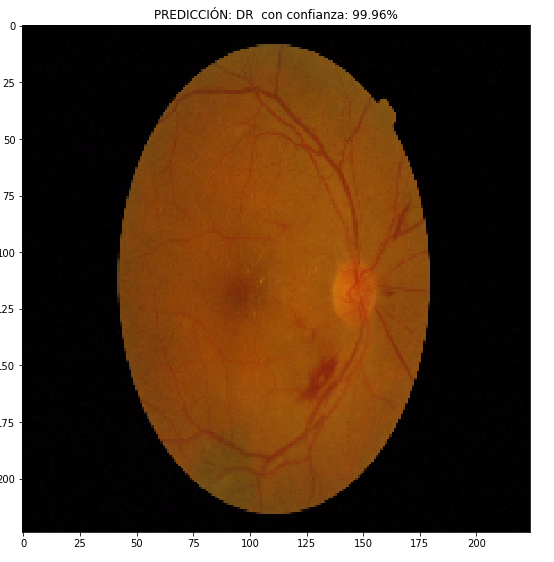
\includegraphics[width=0.7\textwidth,height=\textheight]{source/figures/dr1.png}
\caption{Salida de la segunda etapa del Sistema Multietapa para una
imagen de una retina enferma de RD \label{dr1}}
\end{figure}

\begin{figure}
\centering
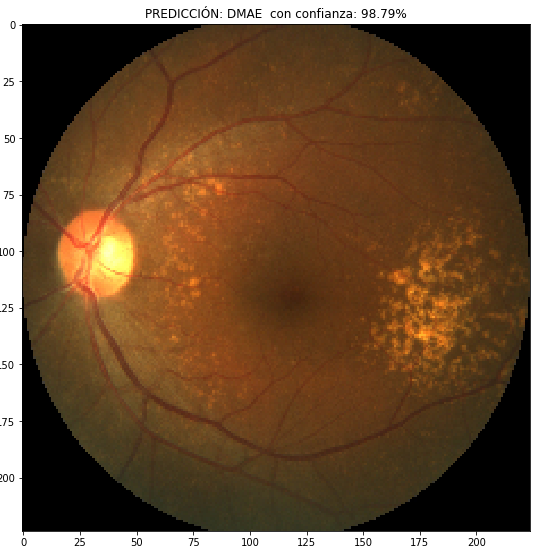
\includegraphics[width=0.7\textwidth,height=\textheight]{source/figures/dr2.png}
\caption{Salida de la segunda etapa del Sistema Multietapa para una
imagen de una retina enferma de DMAE \label{dr2}}
\end{figure}

Los resultados en esta segunda etapa son mucho más satisfactorios que
los de la primera, obteniéndose la máxima \textbf{accuracy} (97.4\%) con
la arquitectura Resnet50, que será la utilizada en el \textbf{Sistema de
Predicción e Interpretación}. Las Figuras \ref{dr1} y \ref{dr2} son dos
ejemplos de la respuesta proporcionada por esta etapa del sistema.

\newpage

\hypertarget{evaluaciuxf3n-del-sistema-3-ensemble-de-clasificadores}{%
\section{Evaluación del Sistema 3: Ensemble de
Clasificadores}\label{evaluaciuxf3n-del-sistema-3-ensemble-de-clasificadores}}

Para este sistema se han evaluado 3 arquitecturas distintas:
\textbf{VGG16, ResNet e InceptionV3}. Como se ha explicado
anteriormente, cada una de estas tres arquitecturas ha sido entrenada
con un subconjunto distinto de los datos. De esta forma se han obtenido
clasificadores no correlados que, al ser combinados, han permitido
obtener un rendimiento superior al de cada uno de ellos de forma
individual.

Para la arquitectura VGG16, al utilizarse la técnica del
\textbf{Transfer Learning}, se han evaluado diferentes versiones,
congelando cada vez distinto número de capas como muestra la tabla
\ref{training4}.

\begin{longtable}[]{@{}lclc@{}}
\caption{Resultados del entrenamiento del sistema 3. Modelos evaluados
con el dataset de validación \label{training4}}\tabularnewline
\toprule
\begin{minipage}[b]{0.22\columnwidth}\raggedright
train blocks\strut
\end{minipage} & \begin{minipage}[b]{0.11\columnwidth}\centering
LR\strut
\end{minipage} & \begin{minipage}[b]{0.15\columnwidth}\raggedright
accuracy\strut
\end{minipage} & \begin{minipage}[b]{0.11\columnwidth}\centering
loss\strut
\end{minipage}\tabularnewline
\midrule
\endfirsthead
\toprule
\begin{minipage}[b]{0.22\columnwidth}\raggedright
train blocks\strut
\end{minipage} & \begin{minipage}[b]{0.11\columnwidth}\centering
LR\strut
\end{minipage} & \begin{minipage}[b]{0.15\columnwidth}\raggedright
accuracy\strut
\end{minipage} & \begin{minipage}[b]{0.11\columnwidth}\centering
loss\strut
\end{minipage}\tabularnewline
\midrule
\endhead
\begin{minipage}[t]{0.22\columnwidth}\raggedright
FC\strut
\end{minipage} & \begin{minipage}[t]{0.11\columnwidth}\centering
5e-5\strut
\end{minipage} & \begin{minipage}[t]{0.15\columnwidth}\raggedright
0.6695\strut
\end{minipage} & \begin{minipage}[t]{0.11\columnwidth}\centering
0.6676\strut
\end{minipage}\tabularnewline
\begin{minipage}[t]{0.22\columnwidth}\raggedright
Bloque 5\strut
\end{minipage} & \begin{minipage}[t]{0.11\columnwidth}\centering
5e-5\strut
\end{minipage} & \begin{minipage}[t]{0.15\columnwidth}\raggedright
0.7458\strut
\end{minipage} & \begin{minipage}[t]{0.11\columnwidth}\centering
0.6068\strut
\end{minipage}\tabularnewline
\begin{minipage}[t]{0.22\columnwidth}\raggedright
Bloques 4,5\strut
\end{minipage} & \begin{minipage}[t]{0.11\columnwidth}\centering
5e-6\strut
\end{minipage} & \begin{minipage}[t]{0.15\columnwidth}\raggedright
0.7119\strut
\end{minipage} & \begin{minipage}[t]{0.11\columnwidth}\centering
0.5878\strut
\end{minipage}\tabularnewline
\begin{minipage}[t]{0.22\columnwidth}\raggedright
Bloques 3,4,5\strut
\end{minipage} & \begin{minipage}[t]{0.11\columnwidth}\centering
5e-6\strut
\end{minipage} & \begin{minipage}[t]{0.15\columnwidth}\raggedright
0.7119\strut
\end{minipage} & \begin{minipage}[t]{0.11\columnwidth}\centering
0.5776\strut
\end{minipage}\tabularnewline
\begin{minipage}[t]{0.22\columnwidth}\raggedright
Bloques 2,3,4,5\strut
\end{minipage} & \begin{minipage}[t]{0.11\columnwidth}\centering
5e-6\strut
\end{minipage} & \begin{minipage}[t]{0.15\columnwidth}\raggedright
0.7797\strut
\end{minipage} & \begin{minipage}[t]{0.11\columnwidth}\centering
0.5456\strut
\end{minipage}\tabularnewline
\begin{minipage}[t]{0.22\columnwidth}\raggedright
Todos\strut
\end{minipage} & \begin{minipage}[t]{0.11\columnwidth}\centering
5e-6\strut
\end{minipage} & \begin{minipage}[t]{0.15\columnwidth}\raggedright
0.7458\strut
\end{minipage} & \begin{minipage}[t]{0.11\columnwidth}\centering
0.5973\strut
\end{minipage}\tabularnewline
\bottomrule
\end{longtable}

En este caso, el mejor resultado lo obtenemos dejando congelado el
primer bloque convolucional y entrenando el resto de bloques.

En la tabla \ref{training5} se muestran los resultados del entrenamiento
para otras arquitecturas.

\begin{longtable}[]{@{}lclc@{}}
\caption{Resultados del entrenamiento con diferentes arquitecturas del
sistema 3. Modelos evaluados con el dataset de validación
\label{training5}}\tabularnewline
\toprule
\begin{minipage}[b]{0.22\columnwidth}\raggedright
Arquitectura\strut
\end{minipage} & \begin{minipage}[b]{0.11\columnwidth}\centering
LR\strut
\end{minipage} & \begin{minipage}[b]{0.15\columnwidth}\raggedright
accuracy\strut
\end{minipage} & \begin{minipage}[b]{0.11\columnwidth}\centering
loss\strut
\end{minipage}\tabularnewline
\midrule
\endfirsthead
\toprule
\begin{minipage}[b]{0.22\columnwidth}\raggedright
Arquitectura\strut
\end{minipage} & \begin{minipage}[b]{0.11\columnwidth}\centering
LR\strut
\end{minipage} & \begin{minipage}[b]{0.15\columnwidth}\raggedright
accuracy\strut
\end{minipage} & \begin{minipage}[b]{0.11\columnwidth}\centering
loss\strut
\end{minipage}\tabularnewline
\midrule
\endhead
\begin{minipage}[t]{0.22\columnwidth}\raggedright
InceptionV3 Resnet50\strut
\end{minipage} & \begin{minipage}[t]{0.11\columnwidth}\centering
1e-5 1e-5\strut
\end{minipage} & \begin{minipage}[t]{0.15\columnwidth}\raggedright
0.6076 0.6383\strut
\end{minipage} & \begin{minipage}[t]{0.11\columnwidth}\centering
0.7293 0.7260\strut
\end{minipage}\tabularnewline
\bottomrule
\end{longtable}

El \textbf{ensemble} final usado en el \textbf{Sistema de Predicción e
Interpretación} ha combinado las predicciones de la las dos redes de la
tabla \ref{training5} y la red que ha entrenado los bloques 2, 3, 4 y 5
de la tabla \ref{training4}.

En las Figuras \ref{s331}, \ref{s332} y \ref{s333} se pueden ver
ejemplos de la respuesta proporcionada por este tercer sistema. Como se
puede ver en ellas, existen ocasiones en que alguno de los 3
clasificadores del ensemble proporciona una respuesta equivocada. Sin
embargo, el resultado final proporcionado por el ensemble devuelve la
respuesta correcta. Es en estos casos donde se puede comprobar la
robustez que proporciona haber usado un sistema basado en la combinación
de varios modelos distintos.

\begin{figure}
\centering
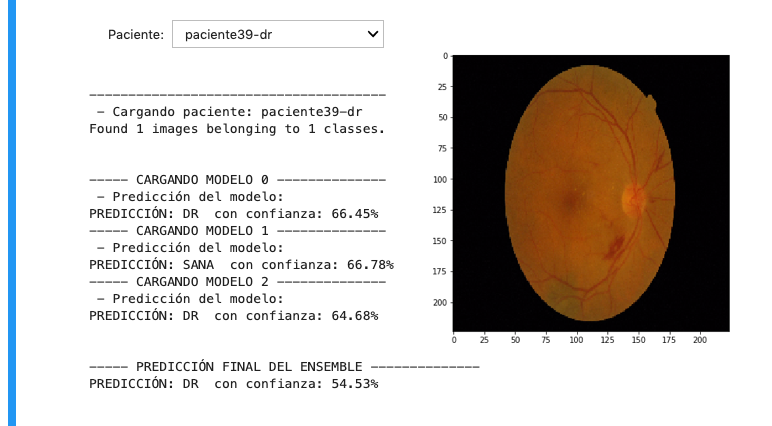
\includegraphics[width=1\textwidth,height=\textheight]{source/figures/s331.png}
\caption{Salida del Sistema 3 para una imagen de una retina enferma de
RD (omitidos los mapas de activación) \label{s331}}
\end{figure}

\begin{figure}
\centering
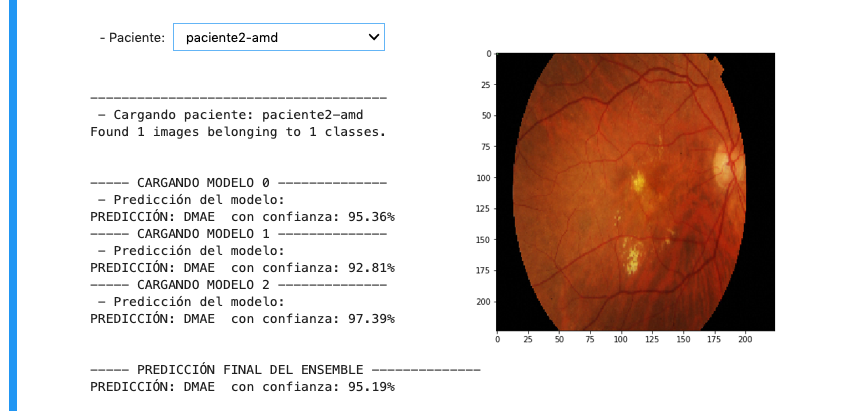
\includegraphics[width=1\textwidth,height=\textheight]{source/figures/s332.png}
\caption{Salida del Sistema 3 para una imagen de una retina enferma de
DMAE (omitidos los mapas de activación) \label{s332}}
\end{figure}

\begin{figure}
\centering
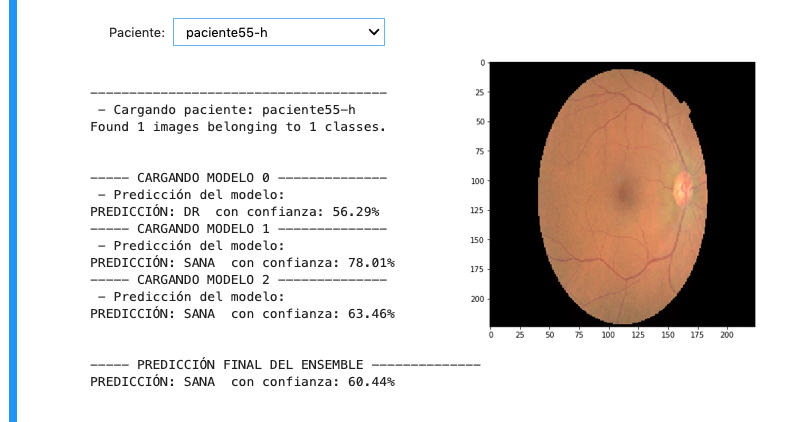
\includegraphics[width=1\textwidth,height=\textheight]{source/figures/s333.png}
\caption{Salida del Sistema 3 para una imagen de una retina sana
(omitidos los mapas de activación) \label{s333}}
\end{figure}

\newpage

\hypertarget{sistema-de-predicciuxf3n-e-interpretaciuxf3n}{%
\section{Sistema de Predicción e
Interpretación}\label{sistema-de-predicciuxf3n-e-interpretaciuxf3n}}

El Sistema de Predicción e Interpretación permite usar todos los modelos
explicados anteriormente simplemente seleccionando una imagen de un
paciente.

En las Figuras \ref{pred1} y \ref{pred2} se muestra el Sistema de
Predicción devolviendo la predicción realizada por las dos etapas del
Sistema 2 para la imagen de un paciente con Degeneración Macular.
Previamente, el usuario ha tenido que añadir la imagen de fondo de ojo a
una carpeta y haber seleccionado el nombre del fichero en el selector de
la parte superior.\footnote{Aunque el nombre del fichero contenga la
  palabra AMD (Age-Related Macular Degeneration, en ningún momento el
  sistema ha utilizado esa información para realizar su predicción.} En
los mapas de atención que devuelve el sistema es posible apreciar cómo
los modelos han basado su predicción en la presencia de \textbf{drusas}.

\begin{figure}
\centering
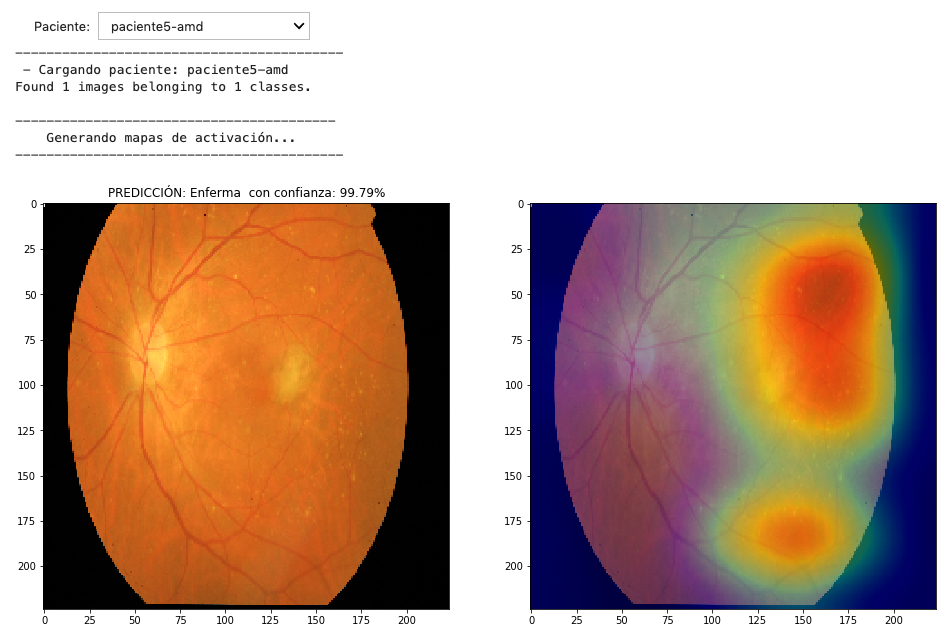
\includegraphics[width=1\textwidth,height=\textheight]{source/figures/pred1.png}
\caption{Respuesta del Sistema de Predicción a la imagen de una retina
con DMAE. Etapa primera del Sistema Multietapa \label{pred1}}
\end{figure}

\begin{figure}
\centering
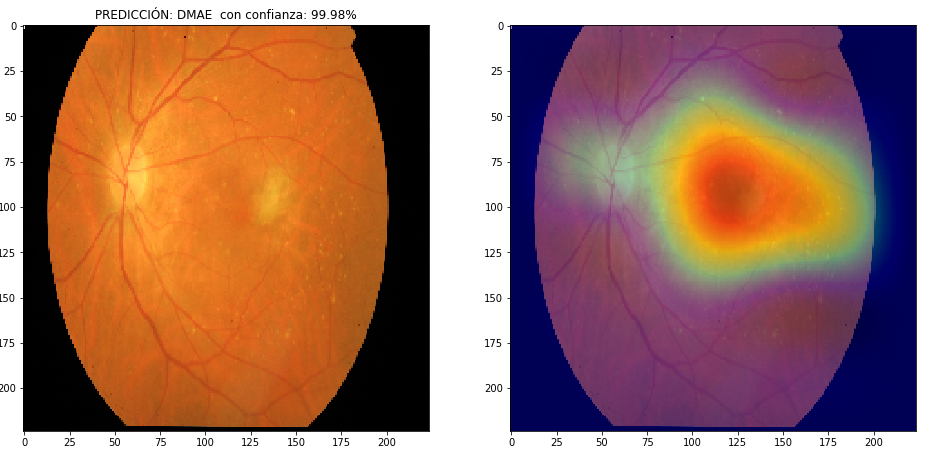
\includegraphics[width=1\textwidth,height=\textheight]{source/figures/pred2.png}
\caption{Respuesta del Sistema de Predicción a la imagen de una retina
con DMAE. Etapa segunda del Sistema Multietapa \label{pred2}}
\end{figure}

\begin{figure}
\centering
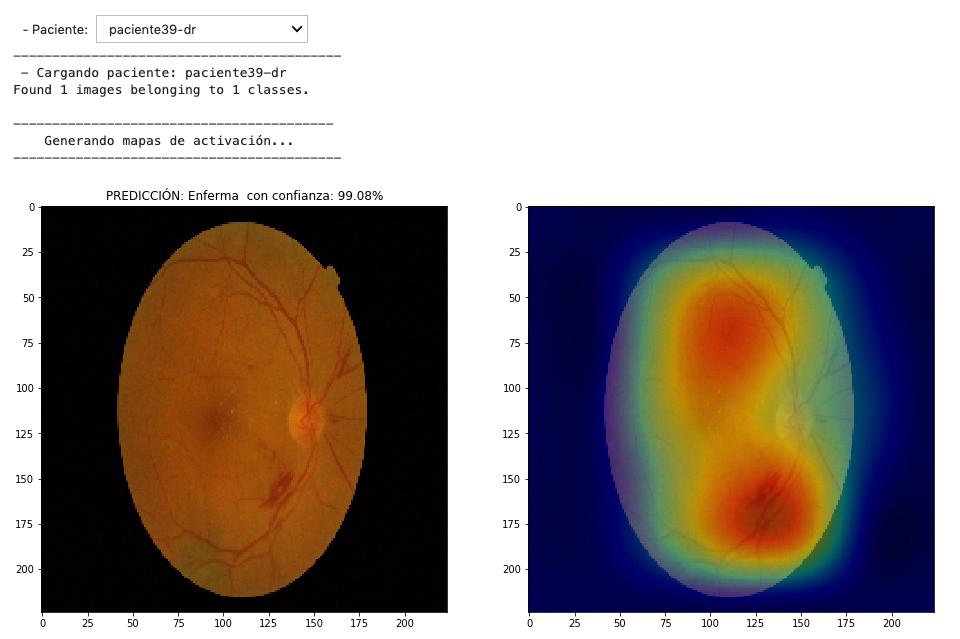
\includegraphics[width=1\textwidth,height=\textheight]{source/figures/pred3.png}
\caption{Respuesta del Sistema de Predicción a la imagen de una retina
con RD. Etapa primera del Sistema Multietapa \label{pred3}}
\end{figure}

\begin{figure}
\centering
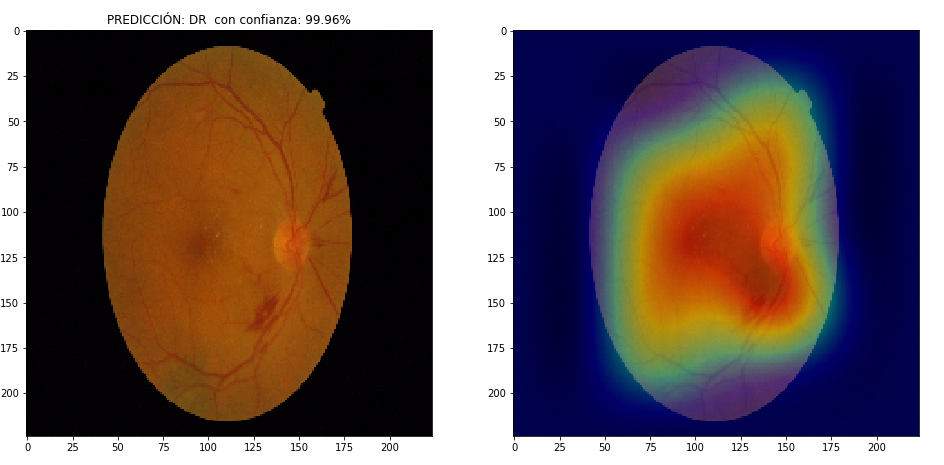
\includegraphics[width=1\textwidth,height=\textheight]{source/figures/pred4.png}
\caption{Respuesta del Sistema de Predicción a la imagen de una retina
con RD. Etapa segunda del Sistema Multietapa \label{pred4}}
\end{figure}

De la misma forma, las Figuras \ref{pred3}, y \ref{pred4} muestran la
respuesta de ese mismo sistema para una retina enferma de RD.

\begin{figure}
\centering
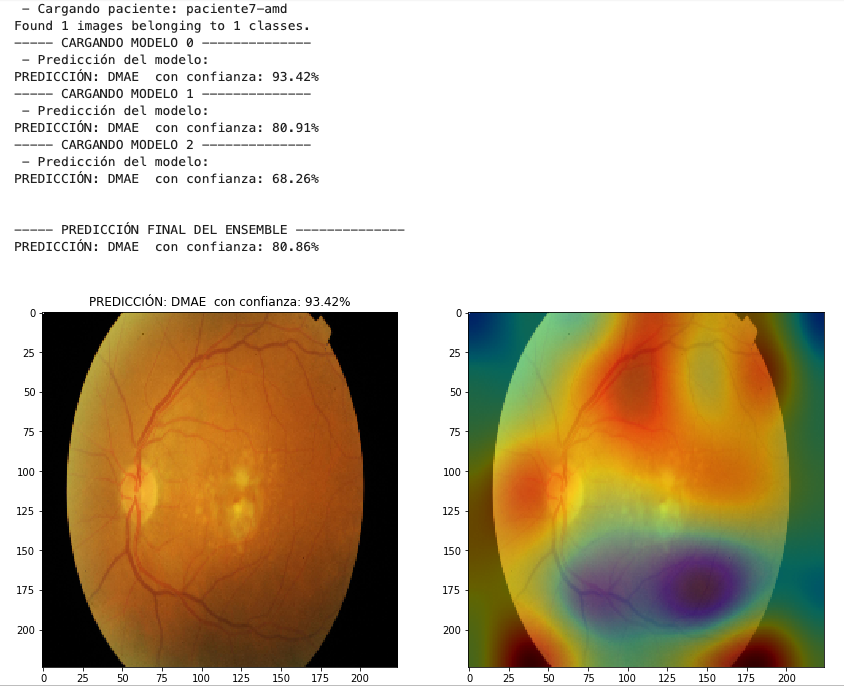
\includegraphics[width=1\textwidth,height=\textheight]{source/figures/pred5.png}
\caption{Respuesta del Sistema de Predicción a la imagen de una retina
con DMAE. Mapa de activación del primer clasificador del Ensemble de
Clasificadores \label{pred5}}
\end{figure}

\begin{figure}
\centering
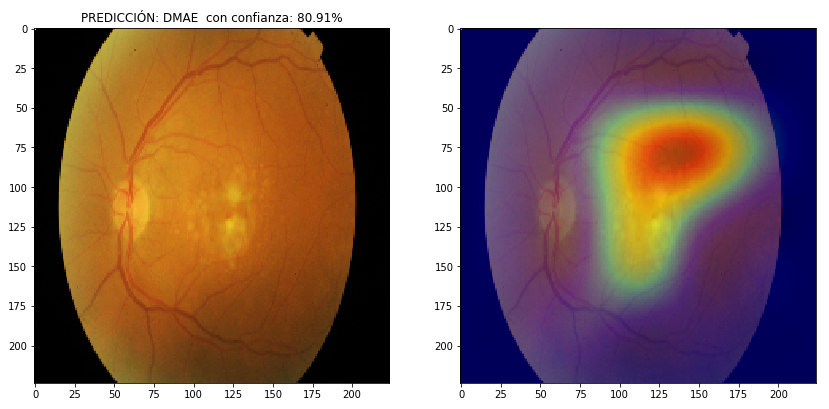
\includegraphics[width=1\textwidth,height=\textheight]{source/figures/pred6.png}
\caption{Respuesta del Sistema de Predicción a la imagen de una retina
con DMAE. Mapa de activación del segundo clasificador del Ensemble de
Clasificadores \label{pred6}}
\end{figure}

\begin{figure}
\centering
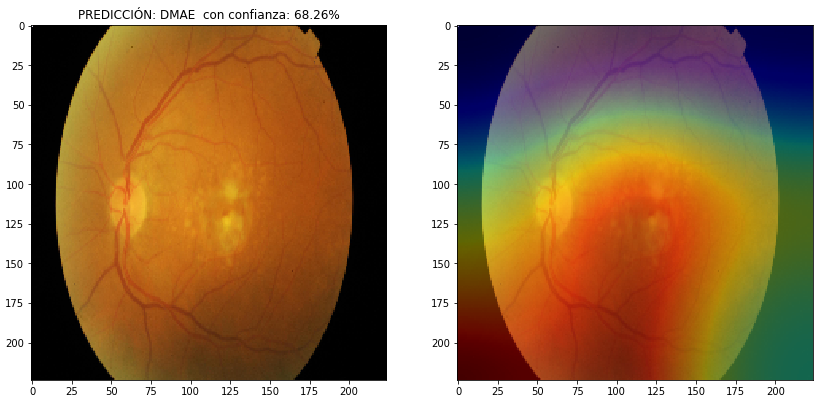
\includegraphics[width=1\textwidth,height=\textheight]{source/figures/pred7.png}
\caption{Respuesta del Sistema de Predicción a la imagen de una retina
con DMAE. Mapa de activación del tercer clasificador del Ensemble de
Clasificadores \label{pred7}}
\end{figure}

La respuesta del \textbf{Ensemble de Clasificadores} para una imagen de
una retina enferma de DMAE, como se aprecia en las Figuras \ref{pred5},
\ref{pred6} y \ref{pred7}, es muy interesante. Mientras que el primer
clasificador basa su clasificación en la posible presencia de
neovascularización (Figura \ref{pred5}), los otros dos clasificadores
(Figuras \ref{pred6} y \ref{pred7}) se basan en la presencia de drusas.

\begin{figure}
\centering
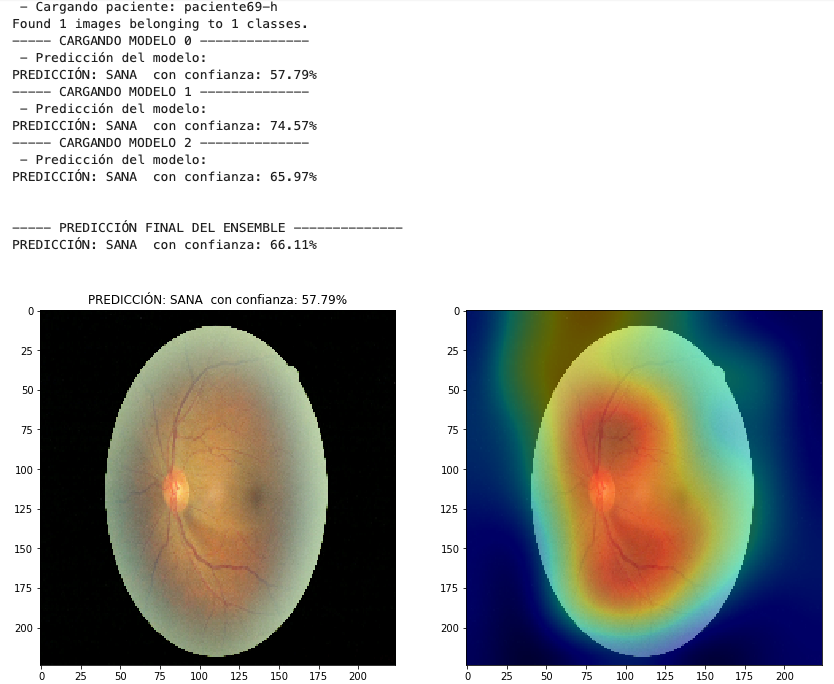
\includegraphics[width=1\textwidth,height=\textheight]{source/figures/pred8.png}
\caption{Respuesta del Sistema de Predicción a la imagen de una retina
sana. Mapa de activación del primer clasificador del Ensemble de
Clasificadores \label{pred8}}
\end{figure}

\begin{figure}
\centering
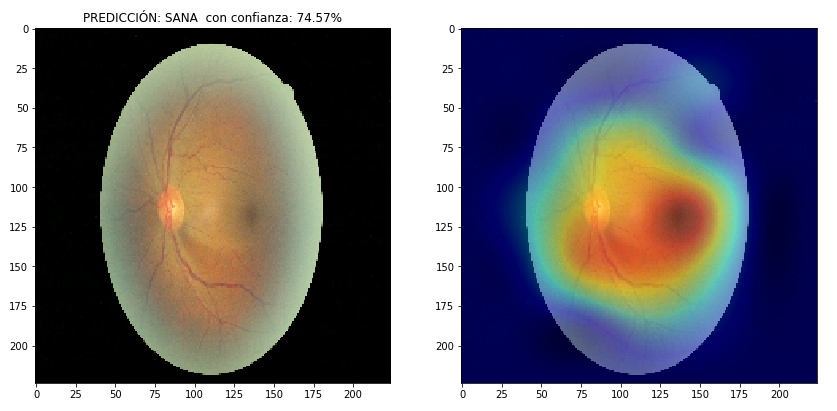
\includegraphics[width=1\textwidth,height=\textheight]{source/figures/pred9.png}
\caption{Respuesta del Sistema de Predicción a la imagen de una retina
sana. Mapa de activación del segundo clasificador del Ensemble de
Clasificadores \label{pred9}}
\end{figure}

\begin{figure}
\centering
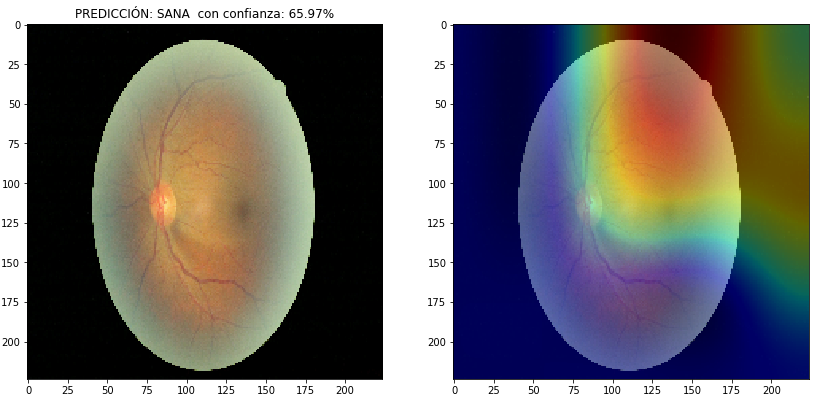
\includegraphics[width=1\textwidth,height=\textheight]{source/figures/pred10.png}
\caption{Respuesta del Sistema de Predicción a la imagen de una retina
sana. Mapa de activación del tercer clasificador del Ensemble de
Clasificadores \label{pred10}}
\end{figure}

Las Figuras \ref{pred8}, \ref{pred9} y \ref{pred10} muestran la salida
del \textbf{Ensemble de Clasificadores} para una imagen de una retina
sana. Este caso también es interesante porque ha permitido detectar un
\textbf{sesgo} en nuestro modelo. La Figura \ref{pred10} muestra cómo
este clasificador basa su predicción en la pequeña muesca que existe en
la parte superior derecha de la imagen de fondo de ojo. Esto se debe a
que, todas las imágenes del dataset de Kaggle presentan esa muesca. Como
ese dataset únicamente contiene imágenes de retinas sanas o retinas con
RD, nuestro clasificador tiene un sesgo y automáticamente descartará la
opción de DMAE cuando vea una imagen de este tipo. Esto puede explicar
también el valor tan alto de \textbf{accuracy} en la segunda etapa del
\textbf{Clasificador Multietapa}. Este sesgo deberá ser corregido en
posteriores versiones del sistema.

\hypertarget{conclusiones}{%
\chapter{Conclusiones}\label{conclusiones}}

En plena era de los datos y la automatización, la medicina no puede
quedar atrás. Las enfermedades analizadas son solo 2 ejemplos de cómo el
Machine Learning puede ayudar a los especialistas a detectar posibles
enfermedades en estadios muy tempranos, lo que nos permitirá tratarlas
antes de que puedan afectar a la vida diaria del paciente.

Durante este trabajo hemos podido comprobar cómo las dos enfermedades
que más casos de ceguera producen en todo el mundo podrían ser
detectadas de forma muy temprana, pudiendo así ser tratadas antes de que
avancen. El uso de clasificadores de Machine Learning entrenados con
datos históricos fiables nos permite crear sistemas robustos que aúnen
todo el conocimiento de los mejores expertos y puedan llegar a todos
estos sitios donde no es fácil encontrar este tipo de especialistas.

Los resultados obtenidos, incluso estando lejos de los de algunos de los
modelos estudiados durante el análisis del estado del arte, son un
motivo de optimismo. Como ya se ha explicado a lo largo del trabajo, la
mayoría de éstos procedían de datasets con una cantidad muy limitada de
imágenes. El sobreajuste, con cantidades tan pequeñas de imágenes es
prácticamente inevitable. Los modelos del estado del arte, cuando se
utilizaran en \emph{el mundo real} con imágenes procedentes de otras
cámaras con distintos tamaños, profundidades de color, artefactos, etc.
tendrán serios problemas para generalizar. Sin embargo, nuestro sistema
está preparado ante todos esos posibles cambios gracias a la gran
cantidad de datasets utilizados, y al uso del \textbf{Data
Augmentation}.

Lejos de buscar el \emph{número bonito}, o el \emph{gran titular}, el
objetivo de este trabajo, como se puso de manifiesto en el capítulo
inicial ha sido siempre crear un sistema verdaderamente \textbf{útil}
para ser introducido en las clínicas. Para ello, es necesario conseguir
un sistema \textbf{robusto} e \textbf{interpretable}. La robustez nos la
proporcionará haber usado más de 39000 imágenes procedentes de 13
conjuntos distintos de datos junto con la combinación de las
predicciones de varios modelos con diferentes arquitecturas. La
interpretabilidad nos la proporcionará el Sistema de Predicción e
Interpretación descrito en apartados anteriores. La información
proporcionada por este sistema como las predicciones parciales con su
correspondiente confianza de cada clasificador o los mapas de atención
ayuda al usuario a entender por qué ha tomado el sistema una decisión
concreta y decidir si es fiable la predicción dada. Aunque sea común oír
aquello de \emph{``Tortura los datos y te confesarán lo que quieras
oír''}, en este caso esa frase no describe la forma de trabajar que ha
sido utilizada.

\hypertarget{trabajo-futuro}{%
\section{Trabajo futuro}\label{trabajo-futuro}}

Una vez creado un sistema inicial verdaderamente útil, robusto y
escalable conseguir esos \emph{números bonitos} de los que hablábamos
anteriormente, requerirá principalmente de tres elementos:
\textbf{nuevas imágenes, mayor pre-procesamiento, y mayor capacidad de
computación para entrenar modelos más complejos}.

El hecho de que el entrenamiento de algunos de los modelos llegara a
durar hasta 96 horas, no ha permitido realizar tantas ejecuciones como
se hubiera deseado. De haber contado con más tiempo o máquinas más
potentes, nuevas arquitecturas como \textbf{Xception}, \textbf{DenseNet}
o \textbf{MobileNet} hubieran sido evaluadas. Además, soluciones de
\textbf{Automated Machine Learning} como \textbf{AutoKeras}\footnote{https://autokeras.com/}
hubieran sido de gran utilidad para la obtención de arquitecturas más
adecuadas al problema analizado.

Aún quedan preguntas en el aire, y no tienen fácil respuesta. Estas
preguntas giran alrededor de cómo sería la puesta en producción de este
sistema en los servicios de salud de todo el mundo. Este sistema nunca
debería ser usado de forma autónoma y, ante la duda, siempre debería
prevalecer la opinión del especialista. Sin embargo, esto no quita que
su implantación en las consultas como complemento a la opinión del
especialista tendría grandes ventajas permitiendo a éste percibir
detalles de los que, quizás, en una primera exploración inicial no se
había percatado. Sólo después de un tiempo de evaluación de esta forma
en consultas, podría empezar a plantearse dotar al sistema de algo más
de autonomía, lo que nos permitiría implementarlo en sistemas de salud
donde la cantidad de especialistas disponibles es muy limitada.

Durante los próximos años de democratización del Machine Learning,
muchos profesionales entenderán que todos estos sistemas no vienen a
sustirtuirlos sino que son una herramienta más de trabajo como lo pueden
ser las tan usadas hojas de cálculo. El Machine Learning está muy lejos
de sustituir a las personas en ámbitos extremadamente complicados como
la medicina. Y hacer una predicción de si esto algún día pasará es poco
más que apostar a un número al azar en una ruleta.

\footnotesize

\hypertarget{referencias}{%
\chapter*{Referencias}\label{referencias}}
\addcontentsline{toc}{chapter}{Referencias}

\hypertarget{refs}{}
\leavevmode\hypertarget{ref-acharya2008application}{}%
Acharya, R. et~al., 2008. Application of higher order spectra for the
identification of diabetes retinopathy stages. \emph{Journal of Medical
Systems}, 32(6), pp.481-488.

\leavevmode\hypertarget{ref-acharya2017automated}{}%
Acharya, U.R. et~al., 2017. Automated screening tool for dry and wet
age-related macular degeneration (ARMD) using pyramid of histogram of
oriented gradients (PHOG) and nonlinear features. \emph{Journal of
Computational Science}, 20, pp.41-51.

\leavevmode\hypertarget{ref-acharya2009computer}{}%
Acharya, U.R. et~al., 2009. Computer-based detection of diabetes
retinopathy stages using digital fundus images. \emph{Proceedings of the
institution of mechanical engineers, part H: journal of engineering in
medicine}, 223(5), pp.545-553.

\leavevmode\hypertarget{ref-acharya2012integrated}{}%
Acharya, U.R. et~al., 2012. An integrated index for the identification
of diabetic retinopathy stages using texture parameters. \emph{Journal
of medical systems}, 36(3), pp.2011-2020.

\leavevmode\hypertarget{ref-ichallenge}{}%
Anón, iChallenge AMD Dataset.

\leavevmode\hypertarget{ref-baldi2014searching}{}%
Baldi, P., Sadowski, P. \& Whiteson, D., 2014. Searching for exotic
particles in high-energy physics with deep learning. \emph{Nature
communications}, 5, p.4308.

\leavevmode\hypertarget{ref-ball2015improving}{}%
Ball, J., Balogh, E. \& Miller, B.T., 2015. \emph{Improving diagnosis in
health care}, National Academies Press.

\leavevmode\hypertarget{ref-bjorvig2002economic}{}%
Bjørvig, S., Johansen, M.A. \& Fossen, K., 2002. An economic analysis of
screening for diabetic retinopathy. \emph{Journal of Telemedicine and
Telecare}, 8(1), pp.32-35.

\leavevmode\hypertarget{ref-burlina2011automatic}{}%
Burlina, P. et~al., 2011. Automatic screening of age-related macular
degeneration and retinal abnormalities. En \emph{2011 Annual
International Conference of the IEEE Engineering in Medicine and Biology
Society}. IEEE, pp. 3962-3966.

\leavevmode\hypertarget{ref-burlina2016detection}{}%
Burlina, P. et~al., 2016. Detection of age-related macular degeneration
via deep learning. En \emph{2016 IEEE 13th International Symposium on
Biomedical Imaging (ISBI)}. IEEE, pp. 184-188.

\leavevmode\hypertarget{ref-cade2008diabetes}{}%
Cade, W.T., 2008. Diabetes-related microvascular and macrovascular
diseases in the physical therapy setting. \emph{Physical therapy},
88(11), pp.1322-1335.

\leavevmode\hypertarget{ref-colas2016deep}{}%
Colas, E. et~al., 2016. Deep learning approach for diabetic retinopathy
screening. \emph{Acta Ophthalmologica}, 94.

\leavevmode\hypertarget{ref-collobert2011natural}{}%
Collobert, R. et~al., 2011. Natural language processing (almost) from
scratch. \emph{Journal of machine learning research}, 12(Aug),
pp.2493-2537.

\leavevmode\hypertarget{ref-costa2017convolutional}{}%
Costa, P. \& Campilho, A., 2017. Convolutional bag of words for diabetic
retinopathy detection from eye fundus images. \emph{IPSJ Transactions on
Computer Vision and Applications}, 9(1), p.10.

\leavevmode\hypertarget{ref-cruz2013deep}{}%
Cruz-Roa, A.A. et~al., 2013. A deep learning architecture for image
representation, visual interpretability and automated basal-cell
carcinoma cancer detection. En \emph{International Conference on Medical
Image Computing and Computer-Assisted Intervention}. Springer, pp.
403-410.

\leavevmode\hypertarget{ref-cuadros2009eyepacs}{}%
Cuadros, J. \& Bresnick, G., 2009. EyePACS: an adaptable telemedicine
system for diabetic retinopathy screening. \emph{Journal of diabetes
science and technology}, 3(3), pp.509-516.

\leavevmode\hypertarget{ref-currie2014addressing}{}%
Currie, J., Lin, W. \& Meng, J., 2014. Addressing antibiotic abuse in
China: An experimental audit study. \emph{Journal of development
economics}, 110, pp.39-51.

\leavevmode\hypertarget{ref-darwin2004origin}{}%
Darwin, C., 2004. \emph{On the origin of species, 1859}, Routledge.

\leavevmode\hypertarget{ref-decenciere2013teleophta}{}%
Decencière, E. et~al., 2013. TeleOphta: Machine learning and image
processing methods for teleophthalmology. \emph{Irbm}, 34(2),
pp.196-203.

\leavevmode\hypertarget{ref-decenciere2014feedback}{}%
Decencière, E. et~al., 2014. Feedback on a publicly distributed image
database: the Messidor database. \emph{Image Analysis \& Stereology},
33(3), pp.231-234.

\leavevmode\hypertarget{ref-de2018clinically}{}%
De Fauw, J. et~al., 2018. Clinically applicable deep learning for
diagnosis and referral in retinal disease. \emph{Nature medicine},
24(9), p.1342.

\leavevmode\hypertarget{ref-deng2013new}{}%
Deng, L., Hinton, G. \& Kingsbury, B., 2013. New types of deep neural
network learning for speech recognition and related applications: An
overview. En \emph{2013 IEEE International Conference on Acoustics,
Speech and Signal Processing}. IEEE, pp. 8599-8603.

\leavevmode\hypertarget{ref-ege2000screening}{}%
Ege, B.M. et~al., 2000. Screening for diabetic retinopathy using
computer based image analysis and statistical classification.
\emph{Computer methods and programs in biomedicine}, 62(3), pp.165-175.

\leavevmode\hypertarget{ref-englmeier2004early}{}%
Englmeier, K. et~al., 2004. Early detection of diabetes retinopathy by
new algorithms for automatic recognition of vascular changes.
\emph{European journal of medical research}, 9(10), pp.473-478.

\leavevmode\hypertarget{ref-escobar2016piloting}{}%
Escobar, G.J. et~al., 2016. Piloting electronic medical record--based
early detection of inpatient deterioration in community hospitals.
\emph{Journal of hospital medicine}, 11, pp.S18-S24.

\leavevmode\hypertarget{ref-farnell2008enhancement}{}%
Farnell, D.J. et~al., 2008. Enhancement of blood vessels in digital
fundus photographs via the application of multiscale line operators.
\emph{Journal of the Franklin institute}, 345(7), pp.748-765.

\leavevmode\hypertarget{ref-fong2004diabetic}{}%
Fong, D.S. et~al., 2004. Diabetic retinopathy. \emph{Diabetes care},
27(10), pp.2540-2553.

\leavevmode\hypertarget{ref-gang2002detection}{}%
Gang, L., Chutatape, O. \& Krishnan, S.M., 2002. Detection and
measurement of retinal vessels in fundus images using amplitude modified
second-order Gaussian filter. \emph{IEEE transactions on Biomedical
Engineering}, 49(2), pp.168-172.

\leavevmode\hypertarget{ref-garcia2017machine}{}%
Garcı́a-Floriano, A. et~al., 2017. A machine learning approach to medical
image classification: Detecting age-related macular degeneration in
fundus images. \emph{Computers \& Electrical Engineering}.

\leavevmode\hypertarget{ref-gargeya2017automated}{}%
Gargeya, R. \& Leng, T., 2017. Automated identification of diabetic
retinopathy using deep learning. \emph{Ophthalmology}, 124(7),
pp.962-969.

\leavevmode\hypertarget{ref-giancardo2012exudate}{}%
Giancardo, L. et~al., 2012. Exudate-based diabetic macular edema
detection in fundus images using publicly available datasets.
\emph{Medical image analysis}, 16(1), pp.216-226.

\leavevmode\hypertarget{ref-gondal2017weakly}{}%
Gondal, W.M. et~al., 2017. Weakly-supervised localization of diabetic
retinopathy lesions in retinal fundus images. En \emph{2017 IEEE
International Conference on Image Processing (ICIP)}. IEEE, pp.
2069-2073.

\leavevmode\hypertarget{ref-Goodfellow-et-al-2016}{}%
Goodfellow, I., Bengio, Y. \& Courville, A., 2016. \emph{Deep Learning},
MIT Press.

\leavevmode\hypertarget{ref-grassmann2018deep}{}%
Grassmann, F. et~al., 2018. A deep learning algorithm for prediction of
age-related eye disease study severity scale for age-related macular
degeneration from color fundus photography. \emph{Ophthalmology},
125(9), pp.1410-1420.

\leavevmode\hypertarget{ref-age2001randomized}{}%
Group, A.-R.E.D.S.R. \& others, 2001. A randomized, placebo-controlled,
clinical trial of high-dose supplementation with vitamins C and E, beta
carotene, and zinc for age-related macular degeneration and vision loss:
AREDS report no. 8. \emph{Archives of ophthalmology}, 119(10), p.1417.

\leavevmode\hypertarget{ref-early1991grading}{}%
Group, E.T.D.R.S.R. \& others, 1991. Grading diabetic retinopathy from
stereoscopic color fundus photographs---an extension of the modified
Airlie House classification: ETDRS report number 10.
\emph{Ophthalmology}, 98(5), pp.786-806.

\leavevmode\hypertarget{ref-guariguata2014global}{}%
Guariguata, L. et~al., 2014. Global estimates of diabetes prevalence for
2013 and projections for 2035. \emph{Diabetes research and clinical
practice}, 103(2), pp.137-149.

\leavevmode\hypertarget{ref-gulshan2016development}{}%
Gulshan, V. et~al., 2016. Development and validation of a deep learning
algorithm for detection of diabetic retinopathy in retinal fundus
photographs. \emph{Jama}, 316(22), pp.2402-2410.

\leavevmode\hypertarget{ref-hatanaka2008improvement}{}%
Hatanaka, Y. et~al., 2008. Improvement of automatic hemorrhage detection
methods using brightness correction on fundus images. En \emph{Medical
Imaging 2008: Computer-Aided Diagnosis}. International Society for
Optics; Photonics, p. 69153E.

\leavevmode\hypertarget{ref-hayashi2001development}{}%
Hayashi, J. et~al., 2001. A development of computer-aided diagnosis
system using fundus images. En \emph{Proceedings Seventh International
Conference on Virtual Systems and Multimedia}. IEEE, pp. 429-438.

\leavevmode\hypertarget{ref-he2016deep}{}%
He, K. et~al., 2016. Deep residual learning for image recognition. En
\emph{Proceedings of the IEEE conference on computer vision and pattern
recognition}. pp. 770-778.

\leavevmode\hypertarget{ref-helmstaedter2013connectomic}{}%
Helmstaedter, M. et~al., 2013. Connectomic reconstruction of the inner
plexiform layer in the mouse retina. \emph{Nature}, 500(7461), p.168.

\leavevmode\hypertarget{ref-hijazi2010retinal}{}%
Hijazi, M.H.A., Coenen, F. \& Zheng, Y., 2010. Retinal image
classification using a histogram based approach. En \emph{The 2010
International Joint Conference on Neural Networks (IJCNN)}. IEEE, pp.
1-7.

\leavevmode\hypertarget{ref-hoover1998locating}{}%
Hoover, A., Kouznetsova, V. \& Goldbaum, M., 1998. Locating blood
vessels in retinal images by piece-wise threshold probing of a matched
filter response. En \emph{Proceedings of the AMIA Symposium}. American
Medical Informatics Association, p. 931.

\leavevmode\hypertarget{ref-hunter2000quantification}{}%
Hunter, A. et~al., 2000. Quantification of diabetic retinopathy using
neural networks and sensitivity analysis. En \emph{Artificial Neural
Networks in Medicine and Biology}. Springer, pp. 81-86.

\leavevmode\hypertarget{ref-IAPB}{}%
IAPB, 2016. International Agency for the Prevention of Blindness (IAPB).
Diabetic Retinopathy.

\leavevmode\hypertarget{ref-idf2017}{}%
IDF, 2017. IDF Diabetes Atlas 8th Edition 2017.

\leavevmode\hypertarget{ref-jelinek2006automated}{}%
Jelinek, H.J. et~al., 2006. An automated microaneurysm detector as a
tool for identification of diabetic retinopathy in rural optometric
practice. \emph{Clinical and Experimental Optometry}, 89(5), pp.299-305.

\leavevmode\hypertarget{ref-jiang2018trust}{}%
Jiang, H. et~al., 2018. To trust or not to trust a classifier. En
\emph{Advances in Neural Information Processing Systems}. pp. 5541-5552.

\leavevmode\hypertarget{ref-kankanahalli2013automated}{}%
Kankanahalli, S. et~al., 2013. Automated classification of severity of
age-related macular degeneration from fundus photographs.
\emph{Investigative ophthalmology \& visual science}, 54(3),
pp.1789-1796.

\leavevmode\hypertarget{ref-katz1989detection}{}%
Katz, N. et~al., 1989. Detection of blood vessels in retinal images
using two-dimensional matched filters. \emph{IEEE Trans. Med. Imaging},
8(3), pp.263-269.

\leavevmode\hypertarget{ref-kauppi2006diaretdb0}{}%
Kauppi, T. et~al., 2006. DIARETDB0: Evaluation database and methodology
for diabetic retinopathy algorithms. \emph{Machine Vision and Pattern
Recognition Research Group, Lappeenranta University of Technology,
Finland}, 73, pp.1-17.

\leavevmode\hypertarget{ref-klein1984wisconsin}{}%
Klein, R. et~al., 1984. The Wisconsin Epidemiologic Study of Diabetic
Retinopathy: III. Prevalence and risk of diabetic retinopathy when age
at diagnosis is 30 or more years. \emph{Archives of ophthalmology},
102(4), pp.527-532.

\leavevmode\hypertarget{ref-krizhevsky2012imagenet}{}%
Krizhevsky, A., Sutskever, I. \& Hinton, G.E., 2012. Imagenet
classification with deep convolutional neural networks. En
\emph{Advances in neural information processing systems}. pp. 1097-1105.

\leavevmode\hypertarget{ref-lecun2015deep}{}%
LeCun, Y., Bengio, Y. \& Hinton, G., 2015. Deep learning. \emph{nature},
521(7553), p.436.

\leavevmode\hypertarget{ref-lecun1998gradient}{}%
LeCun, Y. et~al., 1998. Gradient-based learning applied to document
recognition. \emph{Proceedings of the IEEE}, 86(11), pp.2278-2324.

\leavevmode\hypertarget{ref-li2000fundus}{}%
Li, H. \& Chutatape, O., 2000. Fundus image features extraction. En
\emph{Proceedings of the 22nd Annual International Conference of the
IEEE Engineering in Medicine and Biology Society (Cat. No. 00CH37143)}.
IEEE, pp. 3071-3073.

\leavevmode\hypertarget{ref-li2017convolutional}{}%
Li, X. et~al., 2017. Convolutional neural networks based transfer
learning for diabetic retinopathy fundus image classification. En
\emph{2017 10th International Congress on Image and Signal Processing,
BioMedical Engineering and Informatics (CISP-BMEI)}. IEEE, pp. 1-11.

\leavevmode\hypertarget{ref-lipton2016mythos}{}%
Lipton, Z.C., 2016. The mythos of model interpretability. \emph{arXiv
preprint arXiv:1606.03490}.

\leavevmode\hypertarget{ref-lowell2004optic}{}%
Lowell, J. et~al., 2004. Optic nerve head segmentation. \emph{IEEE
Transactions on medical Imaging}, 23(2), pp.256-264.

\leavevmode\hypertarget{ref-mandel2016smart}{}%
Mandel, J.C. et~al., 2016. SMART on FHIR: a standards-based,
interoperable apps platform for electronic health records. \emph{Journal
of the American Medical Informatics Association}, 23(5), pp.899-908.

\leavevmode\hypertarget{ref-maninis2016deep}{}%
Maninis, K.-K. et~al., 2016. Deep retinal image understanding. En
\emph{International conference on medical image computing and
computer-assisted intervention}. Springer, pp. 140-148.

\leavevmode\hypertarget{ref-mansour2018deep}{}%
Mansour, R.F., 2018. Deep-learning-based automatic computer-aided
diagnosis system for diabetic retinopathy. \emph{Biomedical engineering
letters}, 8(1), pp.41-57.

\leavevmode\hypertarget{ref-mansour2017evolutionary}{}%
Mansour, R.F., 2017. Evolutionary computing enriched computer-aided
diagnosis system for diabetic retinopathy: a survey. \emph{IEEE reviews
in biomedical engineering}, 10, pp.334-349.

\leavevmode\hypertarget{ref-mookiah2013computer}{}%
Mookiah, M.R.K. et~al., 2013. Computer-aided diagnosis of diabetic
retinopathy: A review. \emph{Computers in biology and medicine}, 43(12),
pp.2136-2155.

\leavevmode\hypertarget{ref-mookiah2014automated}{}%
Mookiah, M.R.K. et~al., 2014. Automated diagnosis of age-related macular
degeneration using greyscale features from digital fundus images.
\emph{Computers in biology and medicine}, 53, pp.55-64.

\leavevmode\hypertarget{ref-mookiah2014decision}{}%
Mookiah, M.R.K. et~al., 2014. Decision support system for age-related
macular degeneration using discrete wavelet transform. \emph{Medical \&
biological engineering \& computing}, 52(9), pp.781-796.

\leavevmode\hypertarget{ref-mookiah2013evolutionary}{}%
Mookiah, M.R.K. et~al., 2013. Evolutionary algorithm based classifier
parameter tuning for automatic diabetic retinopathy grading: A hybrid
feature extraction approach. \emph{Knowledge-based systems}, 39,
pp.9-22.

\leavevmode\hypertarget{ref-niemeijer2009retinopathy}{}%
Niemeijer, M. et~al., 2009. Retinopathy online challenge: automatic
detection of microaneurysms in digital color fundus photographs.
\emph{IEEE transactions on medical imaging}, 29(1), pp.185-195.

\leavevmode\hypertarget{ref-odstrcilik2013retinal}{}%
Odstrcilik, J. et~al., 2013. Retinal vessel segmentation by improved
matched filtering: evaluation on a new high-resolution fundus image
database. \emph{IET Image Processing}, 7(4), pp.373-383.

\leavevmode\hypertarget{ref-osareh2002classification}{}%
Osareh, A. et~al., 2002. Classification and localisation of
diabetic-related eye disease. En \emph{European Conference on Computer
Vision}. Springer, pp. 502-516.

\leavevmode\hypertarget{ref-oyster1999human}{}%
Oyster, C.W., 1999. The human eye. \emph{Sunderland, MA: Sinauer}.

\leavevmode\hypertarget{ref-pan2009survey}{}%
Pan, S.J. \& Yang, Q., 2009. A survey on transfer learning. \emph{IEEE
Transactions on knowledge and data engineering}, 22(10), pp.1345-1359.

\leavevmode\hypertarget{ref-pascolini2012global}{}%
Pascolini, D. \& Mariotti, S.P., 2012. Global estimates of visual
impairment: 2010. \emph{British Journal of Ophthalmology}, 96(5),
pp.614-618.

\leavevmode\hypertarget{ref-pead2019automated}{}%
Pead, E. et~al., 2019. Automated detection of age-related macular
degeneration in color fundus photography: a systematic review.
\emph{survey of ophthalmology}, 64(4), pp.498-511.

\leavevmode\hypertarget{ref-phan2016automatic}{}%
Phan, T.V. et~al., 2016. Automatic screening and grading of age-related
macular degeneration from texture analysis of fundus images.
\emph{Journal of ophthalmology}, 2016.

\leavevmode\hypertarget{ref-pratt2016convolutional}{}%
Pratt, H. et~al., 2016. Convolutional neural networks for diabetic
retinopathy. \emph{Procedia Computer Science}, 90, pp.200-205.

\leavevmode\hypertarget{ref-quellec2017deep}{}%
Quellec, G. et~al., 2017. Deep image mining for diabetic retinopathy
screening. \emph{Medical image analysis}, 39, pp.178-193.

\leavevmode\hypertarget{ref-quellec2008optimal}{}%
Quellec, G. et~al., 2008. Optimal wavelet transform for the detection of
microaneurysms in retina photographs. \emph{IEEE transactions on medical
imaging}, 27(9), pp.1230-1241.

\leavevmode\hypertarget{ref-rajkomar2019machine}{}%
Rajkomar, A., Dean, J. \& Kohane, I., 2019. Machine learning in
medicine. \emph{New England Journal of Medicine}, 380(14), pp.1347-1358.

\leavevmode\hypertarget{ref-rajkomar2018scalable}{}%
Rajkomar, A. et~al., 2018. Scalable and accurate deep learning with
electronic health records. \emph{NPJ Digital Medicine}, 1(1), p.18.

\leavevmode\hypertarget{ref-reza2011decision}{}%
Reza, A.W. \& Eswaran, C., 2011. A decision support system for automatic
screening of non-proliferative diabetic retinopathy. \emph{Journal of
medical systems}, 35(1), pp.17-24.

\leavevmode\hypertarget{ref-ruamviboonsuk2005screening}{}%
Ruamviboonsuk, P. et~al., 2005. Screening for diabetic retinopathy in
rural area using single-field, digital fundus images. \emph{J Med Assoc
Thai}, 88(2), pp.176-180.

\leavevmode\hypertarget{ref-schwartz1970medicine}{}%
Schwartz, W.B., 1970. Medicine and the computer: the promise and
problems of change. En \emph{Use and Impact of Computers in Clinical
Medicine}. Springer, pp. 321-335.

\leavevmode\hypertarget{ref-schwartz1986artificial}{}%
Schwartz, W.B., Patil, R.S. \& Szolovits, P., 1986. Artificial
Intelligence in Medicine Where Do We Stand. \emph{Jurimetrics J.}, 27,
p.362.

\leavevmode\hypertarget{ref-sellahewa2014grader}{}%
Sellahewa, L. et~al., 2014. Grader agreement, and sensitivity and
specificity of digital photography in a community optometry-based
diabetic eye screening program. \emph{Clinical Ophthalmology (Auckland,
NZ)}, 8, p.1345.

\leavevmode\hypertarget{ref-selvaraju2017grad}{}%
Selvaraju, R.R. et~al., 2017. Grad-cam: Visual explanations from deep
networks via gradient-based localization. En \emph{Proceedings of the
IEEE International Conference on Computer Vision}. pp. 618-626.

\leavevmode\hypertarget{ref-simonyan2014very}{}%
Simonyan, K. \& Zisserman, A., 2014. Very deep convolutional networks
for large-scale image recognition. \emph{arXiv preprint
arXiv:1409.1556}.

\leavevmode\hypertarget{ref-sinthanayothin2002automated}{}%
Sinthanayothin, C. et~al., 2002. Automated detection of diabetic
retinopathy on digital fundus images. \emph{Diabetic medicine}, 19(2),
pp.105-112.

\leavevmode\hypertarget{ref-sinthanayothin2003automated}{}%
Sinthanayothin, C. et~al., 2003. Automated screening system for diabetic
retinopathy. En \emph{3rd International Symposium on Image and Signal
Processing and Analysis, 2003. ISPA 2003. Proceedings of the}. IEEE, pp.
915-920.

\leavevmode\hypertarget{ref-slack1966computer}{}%
Slack, W.V. et~al., 1966. A computer-based medical-history system.
\emph{New England Journal of Medicine}, 274(4), pp.194-198.

\leavevmode\hypertarget{ref-szegedy2015going}{}%
Szegedy, C. et~al., 2015. Going deeper with convolutions. En
\emph{Proceedings of the IEEE conference on computer vision and pattern
recognition}. pp. 1-9.

\leavevmode\hypertarget{ref-szegedy2016rethinking}{}%
Szegedy, C. et~al., 2016. Rethinking the inception architecture for
computer vision. En \emph{Proceedings of the IEEE conference on computer
vision and pattern recognition}. pp. 2818-2826.

\leavevmode\hypertarget{ref-tan2018age}{}%
Tan, J.H. et~al., 2018. Age-related macular degeneration detection using
deep convolutional neural network. \emph{Future Generation Computer
Systems}, 87, pp.127-135.

\leavevmode\hypertarget{ref-tolias1998fuzzy}{}%
Tolias, Y.A. \& Panas, S.M., 1998. A fuzzy vessel tracking algorithm for
retinal images based on fuzzy clustering. \emph{IEEE Transactions on
Medical Imaging}, 17(2), pp.263-273.

\leavevmode\hypertarget{ref-vlachos2010multi}{}%
Vlachos, M. \& Dermatas, E., 2010. Multi-scale retinal vessel
segmentation using line tracking. \emph{Computerized Medical Imaging and
Graphics}, 34(3), pp.213-227.

\leavevmode\hypertarget{ref-walter2007automatic}{}%
Walter, T. et~al., 2007. Automatic detection of microaneurysms in color
fundus images. \emph{Medical image analysis}, 11(6), pp.555-566.

\leavevmode\hypertarget{ref-wang2000effective}{}%
Wang, H. et~al., 2000. An effective approach to detect lesions in color
retinal images. En \emph{Proceedings IEEE Conference on Computer Vision
and Pattern Recognition. CVPR 2000 (Cat. No. PR00662)}. IEEE, pp.
181-186.

\leavevmode\hypertarget{ref-world2013universal}{}%
WHO \& others, 2013. Universal eye health: a global action plan
2014-2019.

\leavevmode\hypertarget{ref-williams2004epidemiology}{}%
Williams, R. et~al., 2004. Epidemiology of diabetic retinopathy and
macular oedema: a systematic review. \emph{Eye}, 18(10), p.963.

\leavevmode\hypertarget{ref-wong2014global}{}%
Wong, W.L. et~al., 2014. Global prevalence of age-related macular
degeneration and disease burden projection for 2020 and 2040: a
systematic review and meta-analysis. \emph{The Lancet Global Health},
2(2), pp.e106-e116.

\leavevmode\hypertarget{ref-zhang2009economic}{}%
Zhang, P. et~al., 2009. Economic impact of diabetes. \emph{Diabetes
Atlas, IDF}, 4.

\leavevmode\hypertarget{ref-zhang2018visual}{}%
Zhang, Q.-s. \& Zhu, S.-C., 2018. Visual interpretability for deep
learning: a survey. \emph{Frontiers of Information Technology \&
Electronic Engineering}, 19(1), pp.27-39.

\leavevmode\hypertarget{ref-zhang2017direct}{}%
Zhang, X. et~al., 2017. Direct medical cost associated with diabetic
retinopathy severity in type 2 diabetes in Singapore. \emph{PloS one},
12(7), p.e0180949.

\leavevmode\hypertarget{ref-zheng2012worldwide}{}%
Zheng, Y., He, M. \& Congdon, N., 2012. The worldwide epidemic of
diabetic retinopathy. \emph{Indian journal of ophthalmology}, 60(5),
p.428.

\leavevmode\hypertarget{ref-zheng2012automated}{}%
Zheng, Y., Hijazi, M.H.A. \& Coenen, F., 2012. Automated «disease/no
disease» grading of age-related macular degeneration by an image mining
approach. \emph{Investigative ophthalmology \& visual science}, 53(13),
pp.8310-8318.

\leavevmode\hypertarget{ref-zheng2011automated}{}%
Zheng, Y., Hijazi, M.H.A. \& Coenen, F., 2011. Automated Grading of
Age-Related Macular Degeneration by an Image Mining Approach.
\emph{Investigative Ophthalmology \& Visual Science}, 52(14),
pp.6568-6568.

\leavevmode\hypertarget{ref-zhu2001eye}{}%
Zhu, J., Zhang, E. \& Del Rio-Tsonis, K., 2001. Eye Anatomy. \emph{e
LS}.

\end{document}
